\documentclass[twoside]{book}

% Packages required by doxygen
\usepackage{fixltx2e}
\usepackage{calc}
\usepackage{doxygen}
\usepackage[export]{adjustbox} % also loads graphicx
\usepackage{graphicx}
\usepackage[utf8]{inputenc}
\usepackage{makeidx}
\usepackage{multicol}
\usepackage{multirow}
\PassOptionsToPackage{warn}{textcomp}
\usepackage{textcomp}
\usepackage[nointegrals]{wasysym}
\usepackage[table]{xcolor}

% Font selection
\usepackage[T1]{fontenc}
\usepackage[scaled=.90]{helvet}
\usepackage{courier}
\usepackage{amssymb}
\usepackage{sectsty}
\renewcommand{\familydefault}{\sfdefault}
\allsectionsfont{%
  \fontseries{bc}\selectfont%
  \color{darkgray}%
}
\renewcommand{\DoxyLabelFont}{%
  \fontseries{bc}\selectfont%
  \color{darkgray}%
}
\newcommand{\+}{\discretionary{\mbox{\scriptsize$\hookleftarrow$}}{}{}}

% Page & text layout
\usepackage{geometry}
\geometry{%
  a4paper,%
  top=2.5cm,%
  bottom=2.5cm,%
  left=2.5cm,%
  right=2.5cm%
}
\tolerance=750
\hfuzz=15pt
\hbadness=750
\setlength{\emergencystretch}{15pt}
\setlength{\parindent}{0cm}
\setlength{\parskip}{3ex plus 2ex minus 2ex}
\makeatletter
\renewcommand{\paragraph}{%
  \@startsection{paragraph}{4}{0ex}{-1.0ex}{1.0ex}{%
    \normalfont\normalsize\bfseries\SS@parafont%
  }%
}
\renewcommand{\subparagraph}{%
  \@startsection{subparagraph}{5}{0ex}{-1.0ex}{1.0ex}{%
    \normalfont\normalsize\bfseries\SS@subparafont%
  }%
}
\makeatother

% Headers & footers
\usepackage{fancyhdr}
\pagestyle{fancyplain}
\fancyhead[LE]{\fancyplain{}{\bfseries\thepage}}
\fancyhead[CE]{\fancyplain{}{}}
\fancyhead[RE]{\fancyplain{}{\bfseries\leftmark}}
\fancyhead[LO]{\fancyplain{}{\bfseries\rightmark}}
\fancyhead[CO]{\fancyplain{}{}}
\fancyhead[RO]{\fancyplain{}{\bfseries\thepage}}
\fancyfoot[LE]{\fancyplain{}{}}
\fancyfoot[CE]{\fancyplain{}{}}
\fancyfoot[RE]{\fancyplain{}{\bfseries\scriptsize Generated by Doxygen }}
\fancyfoot[LO]{\fancyplain{}{\bfseries\scriptsize Generated by Doxygen }}
\fancyfoot[CO]{\fancyplain{}{}}
\fancyfoot[RO]{\fancyplain{}{}}
\renewcommand{\footrulewidth}{0.4pt}
\renewcommand{\chaptermark}[1]{%
  \markboth{#1}{}%
}
\renewcommand{\sectionmark}[1]{%
  \markright{\thesection\ #1}%
}

% Indices & bibliography
\usepackage{natbib}
\usepackage[titles]{tocloft}
\setcounter{tocdepth}{3}
\setcounter{secnumdepth}{5}
\makeindex

% Hyperlinks (required, but should be loaded last)
\usepackage{ifpdf}
\ifpdf
  \usepackage[pdftex,pagebackref=true]{hyperref}
\else
  \usepackage[ps2pdf,pagebackref=true]{hyperref}
\fi
\hypersetup{%
  colorlinks=true,%
  linkcolor=blue,%
  citecolor=blue,%
  unicode%
}

% Custom commands
\newcommand{\clearemptydoublepage}{%
  \newpage{\pagestyle{empty}\cleardoublepage}%
}

\usepackage{caption}
\captionsetup{labelsep=space,justification=centering,font={bf},singlelinecheck=off,skip=4pt,position=top}

%===== C O N T E N T S =====

\begin{document}

% Titlepage & ToC
\hypersetup{pageanchor=false,
             bookmarksnumbered=true,
             pdfencoding=unicode
            }
\pagenumbering{alph}
\begin{titlepage}
\vspace*{7cm}
\begin{center}%
{\Large Intelligent Tic-\/\+Tac-\/\+Toe }\\
\vspace*{1cm}
{\large Generated by Doxygen 1.8.13}\\
\end{center}
\end{titlepage}
\clearemptydoublepage
\pagenumbering{roman}
\tableofcontents
\clearemptydoublepage
\pagenumbering{arabic}
\hypersetup{pageanchor=true}

%--- Begin generated contents ---
\chapter{Intelligent\+Tic\+Tac\+Toe}
\label{md__r_e_a_d_m_e}
\Hypertarget{md__r_e_a_d_m_e}
The attempt to create a neural network capable of learning \hyperlink{class_tic_tac_toe}{Tic\+Tac\+Toe}.

\section*{Theoretical background}

\href{http://www.dkriesel.com/_media/science/neuronalenetze-en-zeta2-2col-dkrieselcom.pdf}{\tt Neural Networks (David Kriesel)}

\section*{Getting everything running}


\begin{DoxyEnumerate}
\item Compile the project with the command \textquotesingle{}make\textquotesingle{}!
\item Run the generated binary \textquotesingle{}./\+Intelligent\+Tic\+Tac\+Toe\textquotesingle{}!
\item Use the standard input, to control the programm during runtime (see Commands section)!
\end{DoxyEnumerate}

\section*{Commands}


\begin{DoxyEnumerate}
\item Instruction\+: If you type \textquotesingle{}-\/1\textquotesingle{}, the current time in sec. since the system epoch is taken as seed for the random number generator. If you specify a number, probably from a previous run, this seed is taken and you can generate the same behaviour as in the previous run, useful for debugging!
\item Instruction\+: Specify the way, you want to construct your neural network. Implemented is a fully connected non-\/recurrent network, which is only characterized by the number of hidden neurons, a layered network, characterized by the number of layers and the number of neurons per layer, and the possibility to load an already trained network from file, specified by the file name. 3a-\/b. Instruction\+: Depending on the previous choice, you have to give detailed information on your neural network.
\item Instruction\+: From now on you have to specify simulation details. You are asked, if you want to train the neural network against a human, an implemented automated player based on an algorithm, or against itself. The human option should be used only for playing against an already trained network, since the training process takes at least 10.\+000 games to be significantly.
\item Instruction\+: Now you have to specify the learning rate for this simulation run.
\item Instruction\+: Specify the number of games, the simulation should run with the previous given configuration.
\end{DoxyEnumerate}

The simulation should run now and give you information on how long the training process takes. During the training process a file is generated and written to. The win\+Series.\+txt, where a value for each game is given, with reaching 1=100\% being a very sophisticated game. At the end of each simulation the current state of the network is printed to \textquotesingle{}network.\+nn\textquotesingle{} and can be used to laod into a different training session. Both files get overwritten after a new simulation run. At the end the programm doesn\textquotesingle{}t terminate but steps 4-\/6 are repated. To exit the programm, press \textquotesingle{}Ctrl-\/C\textquotesingle{}! 
\chapter{Namespace Index}
\section{Namespace List}
Here is a list of all namespaces with brief descriptions\+:\begin{DoxyCompactList}
\item\contentsline{section}{\hyperlink{namespaceplot_data}{plot\+Data} }{\pageref{namespaceplot_data}}{}
\end{DoxyCompactList}

\chapter{Hierarchical Index}
\section{Class Hierarchy}
This inheritance list is sorted roughly, but not completely, alphabetically\+:\begin{DoxyCompactList}
\item \contentsline{section}{Loading\+Bar}{\pageref{class_loading_bar}}{}
\item \contentsline{section}{Move}{\pageref{struct_move}}{}
\item \contentsline{section}{Neural\+Network}{\pageref{class_neural_network}}{}
\item \contentsline{section}{Neuron}{\pageref{class_neuron}}{}
\item \contentsline{section}{Player}{\pageref{class_player}}{}
\begin{DoxyCompactList}
\item \contentsline{section}{AI}{\pageref{class_a_i}}{}
\item \contentsline{section}{Human}{\pageref{class_human}}{}
\item \contentsline{section}{Logic\+Player}{\pageref{class_logic_player}}{}
\end{DoxyCompactList}
\item \contentsline{section}{Runner}{\pageref{class_runner}}{}
\item \contentsline{section}{Synapse}{\pageref{class_synapse}}{}
\item \contentsline{section}{Tic\+Tac\+Toe}{\pageref{class_tic_tac_toe}}{}
\end{DoxyCompactList}

\chapter{Class Index}
\section{Class List}
Here are the classes, structs, unions and interfaces with brief descriptions\+:\begin{DoxyCompactList}
\item\contentsline{section}{\hyperlink{class_a_i}{AI} }{\pageref{class_a_i}}{}
\item\contentsline{section}{\hyperlink{class_human}{Human} }{\pageref{class_human}}{}
\item\contentsline{section}{\hyperlink{class_loading_bar}{Loading\+Bar} }{\pageref{class_loading_bar}}{}
\item\contentsline{section}{\hyperlink{class_logic_player}{Logic\+Player} }{\pageref{class_logic_player}}{}
\item\contentsline{section}{\hyperlink{struct_move}{Move} }{\pageref{struct_move}}{}
\item\contentsline{section}{\hyperlink{class_neural_network}{Neural\+Network} }{\pageref{class_neural_network}}{}
\item\contentsline{section}{\hyperlink{class_neuron}{Neuron} }{\pageref{class_neuron}}{}
\item\contentsline{section}{\hyperlink{class_player}{Player} }{\pageref{class_player}}{}
\item\contentsline{section}{\hyperlink{class_runner}{Runner} }{\pageref{class_runner}}{}
\item\contentsline{section}{\hyperlink{class_synapse}{Synapse} }{\pageref{class_synapse}}{}
\item\contentsline{section}{\hyperlink{class_tic_tac_toe}{Tic\+Tac\+Toe} \\*The game \hyperlink{class_tic_tac_toe}{Tic\+Tac\+Toe} }{\pageref{class_tic_tac_toe}}{}
\end{DoxyCompactList}

\chapter{File Index}
\section{File List}
Here is a list of all files with brief descriptions\+:\begin{DoxyCompactList}
\item\contentsline{section}{\hyperlink{ai_8cpp}{ai.\+cpp} }{\pageref{ai_8cpp}}{}
\item\contentsline{section}{\hyperlink{ai_8h}{ai.\+h} }{\pageref{ai_8h}}{}
\item\contentsline{section}{\hyperlink{constants_8cpp}{constants.\+cpp} }{\pageref{constants_8cpp}}{}
\item\contentsline{section}{\hyperlink{constants_8h}{constants.\+h} }{\pageref{constants_8h}}{}
\item\contentsline{section}{\hyperlink{human_8cpp}{human.\+cpp} }{\pageref{human_8cpp}}{}
\item\contentsline{section}{\hyperlink{human_8h}{human.\+h} }{\pageref{human_8h}}{}
\item\contentsline{section}{\hyperlink{loading_bar_8cpp}{loading\+Bar.\+cpp} }{\pageref{loading_bar_8cpp}}{}
\item\contentsline{section}{\hyperlink{loading_bar_8h}{loading\+Bar.\+h} }{\pageref{loading_bar_8h}}{}
\item\contentsline{section}{\hyperlink{logic_player_8cpp}{logic\+Player.\+cpp} }{\pageref{logic_player_8cpp}}{}
\item\contentsline{section}{\hyperlink{logic_player_8h}{logic\+Player.\+h} }{\pageref{logic_player_8h}}{}
\item\contentsline{section}{\hyperlink{main_8cpp}{main.\+cpp} }{\pageref{main_8cpp}}{}
\item\contentsline{section}{\hyperlink{neural_network_8cpp}{neural\+Network.\+cpp} }{\pageref{neural_network_8cpp}}{}
\item\contentsline{section}{\hyperlink{neural_network_8h}{neural\+Network.\+h} }{\pageref{neural_network_8h}}{}
\item\contentsline{section}{\hyperlink{neuron_8cpp}{neuron.\+cpp} }{\pageref{neuron_8cpp}}{}
\item\contentsline{section}{\hyperlink{neuron_8h}{neuron.\+h} }{\pageref{neuron_8h}}{}
\item\contentsline{section}{\hyperlink{player_8cpp}{player.\+cpp} }{\pageref{player_8cpp}}{}
\item\contentsline{section}{\hyperlink{player_8h}{player.\+h} }{\pageref{player_8h}}{}
\item\contentsline{section}{\hyperlink{plot_data_8py}{plot\+Data.\+py} }{\pageref{plot_data_8py}}{}
\item\contentsline{section}{\hyperlink{runner_8cpp}{runner.\+cpp} }{\pageref{runner_8cpp}}{}
\item\contentsline{section}{\hyperlink{runner_8h}{runner.\+h} }{\pageref{runner_8h}}{}
\item\contentsline{section}{\hyperlink{synapse_8cpp}{synapse.\+cpp} }{\pageref{synapse_8cpp}}{}
\item\contentsline{section}{\hyperlink{synapse_8h}{synapse.\+h} }{\pageref{synapse_8h}}{}
\item\contentsline{section}{\hyperlink{tictactoe_8cpp}{tictactoe.\+cpp} }{\pageref{tictactoe_8cpp}}{}
\item\contentsline{section}{\hyperlink{tictactoe_8h}{tictactoe.\+h} }{\pageref{tictactoe_8h}}{}
\end{DoxyCompactList}

\chapter{Namespace Documentation}
\hypertarget{namespaceplot_data}{}\section{plot\+Data Namespace Reference}
\label{namespaceplot_data}\index{plot\+Data@{plot\+Data}}
\subsection*{Variables}
\begin{DoxyCompactItemize}
\item 
list \hyperlink{namespaceplot_data_a3973b174067454c6d6fb4a100600574b}{colors} = \mbox{[}\textquotesingle{}b\textquotesingle{},\textquotesingle{}r\textquotesingle{},\textquotesingle{}y\textquotesingle{},\textquotesingle{}k\textquotesingle{}\mbox{]}
\item 
string \hyperlink{namespaceplot_data_acefbb49a026077f724500d7c511fb59e}{folder} = \textquotesingle{}long\+Run/\textquotesingle{}
\item 
\hyperlink{namespaceplot_data_a44c9f3af3147f385257597dd63d09e3a}{data} = np.\+loadtxt(\hyperlink{namespaceplot_data_acefbb49a026077f724500d7c511fb59e}{folder}+\textquotesingle{}win\+Series.\+txt\textquotesingle{},dtype=float)
\item 
\hyperlink{namespaceplot_data_a654ab80d46bf5af451e1ca85b1dcb573}{error} = np.\+loadtxt(\hyperlink{namespaceplot_data_acefbb49a026077f724500d7c511fb59e}{folder}+\textquotesingle{}error\+Sums.\+txt\textquotesingle{},dtype=float,delimiter=\textquotesingle{};\textquotesingle{})
\item 
\hyperlink{namespaceplot_data_af459551cfb398cc731a4c51c4d44df41}{contraction\+Number} = min(300,len(\hyperlink{namespaceplot_data_a44c9f3af3147f385257597dd63d09e3a}{data})//2$\ast$$\ast$4)
\item 
\hyperlink{namespaceplot_data_a82986c14482fcee60f04f418a09ca49c}{contracted} = \hyperlink{namespaceplot_data_a44c9f3af3147f385257597dd63d09e3a}{data}\mbox{[}0\+:len(\hyperlink{namespaceplot_data_a44c9f3af3147f385257597dd63d09e3a}{data})+1-\/\hyperlink{namespaceplot_data_af459551cfb398cc731a4c51c4d44df41}{contraction\+Number}\mbox{]}
\item 
\hyperlink{namespaceplot_data_a0bf3fb4a650e2f9eea6c07f84bfd3745}{color}
\item 
\hyperlink{namespaceplot_data_a13e86a1d4baebb88c13b21cf4a6e474f}{label}
\item 
\hyperlink{namespaceplot_data_a3bb3a1ce0591a27573ad339091687219}{loc}
\end{DoxyCompactItemize}


\subsection{Variable Documentation}
\mbox{\Hypertarget{namespaceplot_data_a0bf3fb4a650e2f9eea6c07f84bfd3745}\label{namespaceplot_data_a0bf3fb4a650e2f9eea6c07f84bfd3745}} 
\index{plot\+Data@{plot\+Data}!color@{color}}
\index{color@{color}!plot\+Data@{plot\+Data}}
\subsubsection{\texorpdfstring{color}{color}}
{\footnotesize\ttfamily plot\+Data.\+color}



Definition at line 29 of file plot\+Data.\+py.

\mbox{\Hypertarget{namespaceplot_data_a3973b174067454c6d6fb4a100600574b}\label{namespaceplot_data_a3973b174067454c6d6fb4a100600574b}} 
\index{plot\+Data@{plot\+Data}!colors@{colors}}
\index{colors@{colors}!plot\+Data@{plot\+Data}}
\subsubsection{\texorpdfstring{colors}{colors}}
{\footnotesize\ttfamily list plot\+Data.\+colors = \mbox{[}\textquotesingle{}b\textquotesingle{},\textquotesingle{}r\textquotesingle{},\textquotesingle{}y\textquotesingle{},\textquotesingle{}k\textquotesingle{}\mbox{]}}



Definition at line 12 of file plot\+Data.\+py.

\mbox{\Hypertarget{namespaceplot_data_a82986c14482fcee60f04f418a09ca49c}\label{namespaceplot_data_a82986c14482fcee60f04f418a09ca49c}} 
\index{plot\+Data@{plot\+Data}!contracted@{contracted}}
\index{contracted@{contracted}!plot\+Data@{plot\+Data}}
\subsubsection{\texorpdfstring{contracted}{contracted}}
{\footnotesize\ttfamily plot\+Data.\+contracted = \hyperlink{namespaceplot_data_a44c9f3af3147f385257597dd63d09e3a}{data}\mbox{[}0\+:len(\hyperlink{namespaceplot_data_a44c9f3af3147f385257597dd63d09e3a}{data})+1-\/\hyperlink{namespaceplot_data_af459551cfb398cc731a4c51c4d44df41}{contraction\+Number}\mbox{]}}



Definition at line 24 of file plot\+Data.\+py.

\mbox{\Hypertarget{namespaceplot_data_af459551cfb398cc731a4c51c4d44df41}\label{namespaceplot_data_af459551cfb398cc731a4c51c4d44df41}} 
\index{plot\+Data@{plot\+Data}!contraction\+Number@{contraction\+Number}}
\index{contraction\+Number@{contraction\+Number}!plot\+Data@{plot\+Data}}
\subsubsection{\texorpdfstring{contraction\+Number}{contractionNumber}}
{\footnotesize\ttfamily plot\+Data.\+contraction\+Number = min(300,len(\hyperlink{namespaceplot_data_a44c9f3af3147f385257597dd63d09e3a}{data})//2$\ast$$\ast$4)}



Definition at line 20 of file plot\+Data.\+py.

\mbox{\Hypertarget{namespaceplot_data_a44c9f3af3147f385257597dd63d09e3a}\label{namespaceplot_data_a44c9f3af3147f385257597dd63d09e3a}} 
\index{plot\+Data@{plot\+Data}!data@{data}}
\index{data@{data}!plot\+Data@{plot\+Data}}
\subsubsection{\texorpdfstring{data}{data}}
{\footnotesize\ttfamily plot\+Data.\+data = np.\+loadtxt(\hyperlink{namespaceplot_data_acefbb49a026077f724500d7c511fb59e}{folder}+\textquotesingle{}win\+Series.\+txt\textquotesingle{},dtype=float)}



Definition at line 17 of file plot\+Data.\+py.

\mbox{\Hypertarget{namespaceplot_data_a654ab80d46bf5af451e1ca85b1dcb573}\label{namespaceplot_data_a654ab80d46bf5af451e1ca85b1dcb573}} 
\index{plot\+Data@{plot\+Data}!error@{error}}
\index{error@{error}!plot\+Data@{plot\+Data}}
\subsubsection{\texorpdfstring{error}{error}}
{\footnotesize\ttfamily plot\+Data.\+error = np.\+loadtxt(\hyperlink{namespaceplot_data_acefbb49a026077f724500d7c511fb59e}{folder}+\textquotesingle{}error\+Sums.\+txt\textquotesingle{},dtype=float,delimiter=\textquotesingle{};\textquotesingle{})}



Definition at line 18 of file plot\+Data.\+py.

\mbox{\Hypertarget{namespaceplot_data_acefbb49a026077f724500d7c511fb59e}\label{namespaceplot_data_acefbb49a026077f724500d7c511fb59e}} 
\index{plot\+Data@{plot\+Data}!folder@{folder}}
\index{folder@{folder}!plot\+Data@{plot\+Data}}
\subsubsection{\texorpdfstring{folder}{folder}}
{\footnotesize\ttfamily string plot\+Data.\+folder = \textquotesingle{}long\+Run/\textquotesingle{}}



Definition at line 14 of file plot\+Data.\+py.

\mbox{\Hypertarget{namespaceplot_data_a13e86a1d4baebb88c13b21cf4a6e474f}\label{namespaceplot_data_a13e86a1d4baebb88c13b21cf4a6e474f}} 
\index{plot\+Data@{plot\+Data}!label@{label}}
\index{label@{label}!plot\+Data@{plot\+Data}}
\subsubsection{\texorpdfstring{label}{label}}
{\footnotesize\ttfamily plot\+Data.\+label}



Definition at line 29 of file plot\+Data.\+py.

\mbox{\Hypertarget{namespaceplot_data_a3bb3a1ce0591a27573ad339091687219}\label{namespaceplot_data_a3bb3a1ce0591a27573ad339091687219}} 
\index{plot\+Data@{plot\+Data}!loc@{loc}}
\index{loc@{loc}!plot\+Data@{plot\+Data}}
\subsubsection{\texorpdfstring{loc}{loc}}
{\footnotesize\ttfamily plot\+Data.\+loc}



Definition at line 35 of file plot\+Data.\+py.


\chapter{Class Documentation}
\hypertarget{class_a_i}{}\section{AI Class Reference}
\label{class_a_i}\index{AI@{AI}}


{\ttfamily \#include $<$ai.\+h$>$}



Inheritance diagram for AI\+:\nopagebreak
\begin{figure}[H]
\begin{center}
\leavevmode
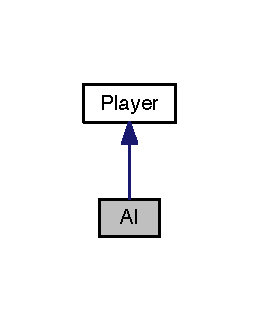
\includegraphics[width=124pt]{class_a_i__inherit__graph}
\end{center}
\end{figure}


Collaboration diagram for AI\+:\nopagebreak
\begin{figure}[H]
\begin{center}
\leavevmode
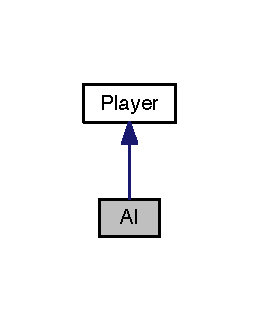
\includegraphics[width=124pt]{class_a_i__coll__graph}
\end{center}
\end{figure}
\subsection*{Public Member Functions}
\begin{DoxyCompactItemize}
\item 
\hyperlink{class_a_i_a24760cc7163907dee1ff7ec9df8fa7af}{AI} (const \hyperlink{ai_8h_aafca5132d037883f5cd25160f7ccdc0d}{Neural\+Network\+Ptr} network\+\_\+)
\item 
\hyperlink{struct_move}{Move} \hyperlink{class_a_i_a2d1a6ed520e3b3ada7133bd03d405d6d}{get\+Move} (\hyperlink{constants_8h_af901d0acc1572fb0c779f84ddd2c6ce8}{Board})
\end{DoxyCompactItemize}


\subsection{Detailed Description}


Definition at line 16 of file ai.\+h.



\subsection{Constructor \& Destructor Documentation}
\mbox{\Hypertarget{class_a_i_a24760cc7163907dee1ff7ec9df8fa7af}\label{class_a_i_a24760cc7163907dee1ff7ec9df8fa7af}} 
\index{AI@{AI}!AI@{AI}}
\index{AI@{AI}!AI@{AI}}
\subsubsection{\texorpdfstring{A\+I()}{AI()}}
{\footnotesize\ttfamily A\+I\+::\+AI (\begin{DoxyParamCaption}\item[{const \hyperlink{ai_8h_aafca5132d037883f5cd25160f7ccdc0d}{Neural\+Network\+Ptr}}]{network\+\_\+ }\end{DoxyParamCaption})}



Definition at line 12 of file ai.\+cpp.



\subsection{Member Function Documentation}
\mbox{\Hypertarget{class_a_i_a2d1a6ed520e3b3ada7133bd03d405d6d}\label{class_a_i_a2d1a6ed520e3b3ada7133bd03d405d6d}} 
\index{AI@{AI}!get\+Move@{get\+Move}}
\index{get\+Move@{get\+Move}!AI@{AI}}
\subsubsection{\texorpdfstring{get\+Move()}{getMove()}}
{\footnotesize\ttfamily \hyperlink{struct_move}{Move} A\+I\+::get\+Move (\begin{DoxyParamCaption}\item[{\hyperlink{constants_8h_af901d0acc1572fb0c779f84ddd2c6ce8}{Board}}]{board }\end{DoxyParamCaption})\hspace{0.3cm}{\ttfamily [virtual]}}



Implements \hyperlink{class_player_a97a516ce71ccef14123884b562c90e4c}{Player}.



Definition at line 16 of file ai.\+cpp.



The documentation for this class was generated from the following files\+:\begin{DoxyCompactItemize}
\item 
\hyperlink{ai_8h}{ai.\+h}\item 
\hyperlink{ai_8cpp}{ai.\+cpp}\end{DoxyCompactItemize}

\hypertarget{class_human}{}\section{Human Class Reference}
\label{class_human}\index{Human@{Human}}


{\ttfamily \#include $<$human.\+h$>$}



Inheritance diagram for Human\+:\nopagebreak
\begin{figure}[H]
\begin{center}
\leavevmode
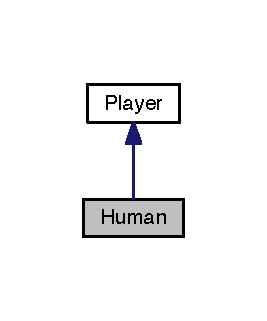
\includegraphics[width=128pt]{class_human__inherit__graph}
\end{center}
\end{figure}


Collaboration diagram for Human\+:\nopagebreak
\begin{figure}[H]
\begin{center}
\leavevmode
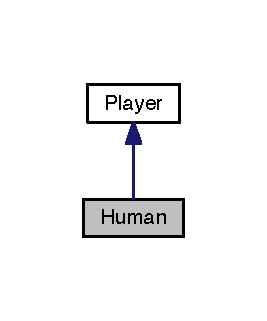
\includegraphics[width=128pt]{class_human__coll__graph}
\end{center}
\end{figure}
\subsection*{Public Member Functions}
\begin{DoxyCompactItemize}
\item 
\hyperlink{class_human_a4f84fcddcedd434023a001eba00a095c}{Human} ()
\item 
\hyperlink{struct_move}{Move} \hyperlink{class_human_a61228d0fbea51c587ea5383d84b152d8}{get\+Move} (\hyperlink{constants_8h_af901d0acc1572fb0c779f84ddd2c6ce8}{Board})
\end{DoxyCompactItemize}


\subsection{Detailed Description}


Definition at line 13 of file human.\+h.



\subsection{Constructor \& Destructor Documentation}
\mbox{\Hypertarget{class_human_a4f84fcddcedd434023a001eba00a095c}\label{class_human_a4f84fcddcedd434023a001eba00a095c}} 
\index{Human@{Human}!Human@{Human}}
\index{Human@{Human}!Human@{Human}}
\subsubsection{\texorpdfstring{Human()}{Human()}}
{\footnotesize\ttfamily Human\+::\+Human (\begin{DoxyParamCaption}{ }\end{DoxyParamCaption})}



Definition at line 10 of file human.\+cpp.



\subsection{Member Function Documentation}
\mbox{\Hypertarget{class_human_a61228d0fbea51c587ea5383d84b152d8}\label{class_human_a61228d0fbea51c587ea5383d84b152d8}} 
\index{Human@{Human}!get\+Move@{get\+Move}}
\index{get\+Move@{get\+Move}!Human@{Human}}
\subsubsection{\texorpdfstring{get\+Move()}{getMove()}}
{\footnotesize\ttfamily \hyperlink{struct_move}{Move} Human\+::get\+Move (\begin{DoxyParamCaption}\item[{\hyperlink{constants_8h_af901d0acc1572fb0c779f84ddd2c6ce8}{Board}}]{board }\end{DoxyParamCaption})\hspace{0.3cm}{\ttfamily [virtual]}}



Implements \hyperlink{class_player_a97a516ce71ccef14123884b562c90e4c}{Player}.



Definition at line 13 of file human.\+cpp.

Here is the call graph for this function\+:\nopagebreak
\begin{figure}[H]
\begin{center}
\leavevmode
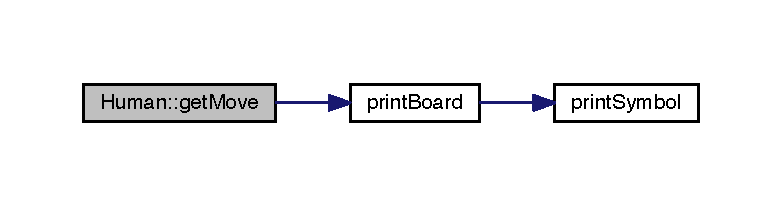
\includegraphics[width=350pt]{class_human_a61228d0fbea51c587ea5383d84b152d8_cgraph}
\end{center}
\end{figure}


The documentation for this class was generated from the following files\+:\begin{DoxyCompactItemize}
\item 
\hyperlink{human_8h}{human.\+h}\item 
\hyperlink{human_8cpp}{human.\+cpp}\end{DoxyCompactItemize}

\hypertarget{class_loading_bar}{}\section{Loading\+Bar Class Reference}
\label{class_loading_bar}\index{Loading\+Bar@{Loading\+Bar}}


{\ttfamily \#include $<$loading\+Bar.\+h$>$}

\subsection*{Public Member Functions}
\begin{DoxyCompactItemize}
\item 
\hyperlink{class_loading_bar_a0afe1dd48a942d6c5e55d7dfe81e3c68}{Loading\+Bar} (string desc\+\_\+=\char`\"{}Progressing\char`\"{})
\item 
void \hyperlink{class_loading_bar_aa36409c317164b0e74f6feafc902fa64}{set} (unsigned length\+\_\+)
\item 
void \hyperlink{class_loading_bar_a0396b27b86129c706371ff81a4991d78}{reset} ()
\item 
void \hyperlink{class_loading_bar_a438e06db16611dd92962d8ebfbb1fe77}{operator++} ()
\item 
void \hyperlink{class_loading_bar_ae9873c79a6760f8ca8d8eac56ff4d4f4}{reprint} ()
\end{DoxyCompactItemize}


\subsection{Detailed Description}


Definition at line 15 of file loading\+Bar.\+h.



\subsection{Constructor \& Destructor Documentation}
\mbox{\Hypertarget{class_loading_bar_a0afe1dd48a942d6c5e55d7dfe81e3c68}\label{class_loading_bar_a0afe1dd48a942d6c5e55d7dfe81e3c68}} 
\index{Loading\+Bar@{Loading\+Bar}!Loading\+Bar@{Loading\+Bar}}
\index{Loading\+Bar@{Loading\+Bar}!Loading\+Bar@{Loading\+Bar}}
\subsubsection{\texorpdfstring{Loading\+Bar()}{LoadingBar()}}
{\footnotesize\ttfamily Loading\+Bar\+::\+Loading\+Bar (\begin{DoxyParamCaption}\item[{string}]{desc\+\_\+ = {\ttfamily \char`\"{}Progressing\char`\"{}} }\end{DoxyParamCaption})}



Definition at line 23 of file loading\+Bar.\+cpp.

Here is the call graph for this function\+:\nopagebreak
\begin{figure}[H]
\begin{center}
\leavevmode
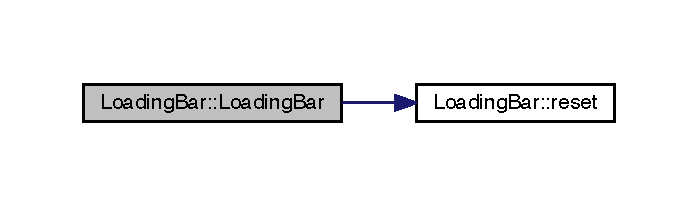
\includegraphics[width=335pt]{class_loading_bar_a0afe1dd48a942d6c5e55d7dfe81e3c68_cgraph}
\end{center}
\end{figure}


\subsection{Member Function Documentation}
\mbox{\Hypertarget{class_loading_bar_a438e06db16611dd92962d8ebfbb1fe77}\label{class_loading_bar_a438e06db16611dd92962d8ebfbb1fe77}} 
\index{Loading\+Bar@{Loading\+Bar}!operator++@{operator++}}
\index{operator++@{operator++}!Loading\+Bar@{Loading\+Bar}}
\subsubsection{\texorpdfstring{operator++()}{operator++()}}
{\footnotesize\ttfamily void Loading\+Bar\+::operator++ (\begin{DoxyParamCaption}{ }\end{DoxyParamCaption})}



Definition at line 46 of file loading\+Bar.\+cpp.

Here is the call graph for this function\+:\nopagebreak
\begin{figure}[H]
\begin{center}
\leavevmode
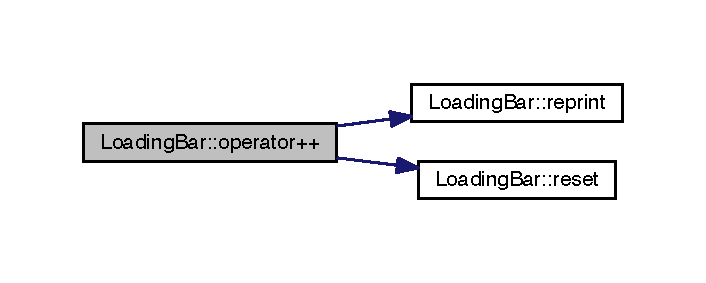
\includegraphics[width=339pt]{class_loading_bar_a438e06db16611dd92962d8ebfbb1fe77_cgraph}
\end{center}
\end{figure}
\mbox{\Hypertarget{class_loading_bar_ae9873c79a6760f8ca8d8eac56ff4d4f4}\label{class_loading_bar_ae9873c79a6760f8ca8d8eac56ff4d4f4}} 
\index{Loading\+Bar@{Loading\+Bar}!reprint@{reprint}}
\index{reprint@{reprint}!Loading\+Bar@{Loading\+Bar}}
\subsubsection{\texorpdfstring{reprint()}{reprint()}}
{\footnotesize\ttfamily void Loading\+Bar\+::reprint (\begin{DoxyParamCaption}{ }\end{DoxyParamCaption})}



Definition at line 74 of file loading\+Bar.\+cpp.

Here is the caller graph for this function\+:\nopagebreak
\begin{figure}[H]
\begin{center}
\leavevmode
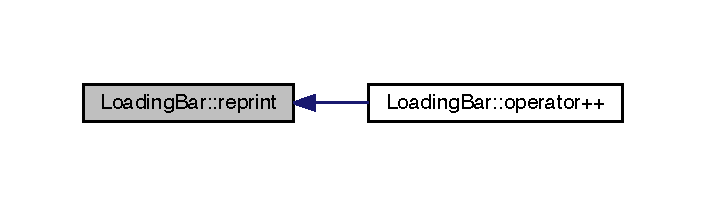
\includegraphics[width=339pt]{class_loading_bar_ae9873c79a6760f8ca8d8eac56ff4d4f4_icgraph}
\end{center}
\end{figure}
\mbox{\Hypertarget{class_loading_bar_a0396b27b86129c706371ff81a4991d78}\label{class_loading_bar_a0396b27b86129c706371ff81a4991d78}} 
\index{Loading\+Bar@{Loading\+Bar}!reset@{reset}}
\index{reset@{reset}!Loading\+Bar@{Loading\+Bar}}
\subsubsection{\texorpdfstring{reset()}{reset()}}
{\footnotesize\ttfamily void Loading\+Bar\+::reset (\begin{DoxyParamCaption}{ }\end{DoxyParamCaption})}



Definition at line 28 of file loading\+Bar.\+cpp.

Here is the caller graph for this function\+:\nopagebreak
\begin{figure}[H]
\begin{center}
\leavevmode
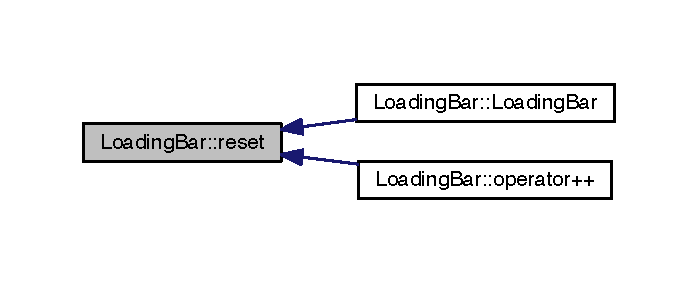
\includegraphics[width=335pt]{class_loading_bar_a0396b27b86129c706371ff81a4991d78_icgraph}
\end{center}
\end{figure}
\mbox{\Hypertarget{class_loading_bar_aa36409c317164b0e74f6feafc902fa64}\label{class_loading_bar_aa36409c317164b0e74f6feafc902fa64}} 
\index{Loading\+Bar@{Loading\+Bar}!set@{set}}
\index{set@{set}!Loading\+Bar@{Loading\+Bar}}
\subsubsection{\texorpdfstring{set()}{set()}}
{\footnotesize\ttfamily void Loading\+Bar\+::set (\begin{DoxyParamCaption}\item[{unsigned}]{length\+\_\+ }\end{DoxyParamCaption})}



Definition at line 37 of file loading\+Bar.\+cpp.

Here is the caller graph for this function\+:\nopagebreak
\begin{figure}[H]
\begin{center}
\leavevmode
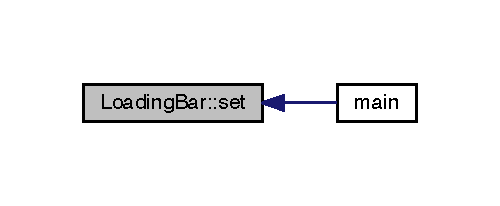
\includegraphics[width=240pt]{class_loading_bar_aa36409c317164b0e74f6feafc902fa64_icgraph}
\end{center}
\end{figure}


The documentation for this class was generated from the following files\+:\begin{DoxyCompactItemize}
\item 
\hyperlink{loading_bar_8h}{loading\+Bar.\+h}\item 
\hyperlink{loading_bar_8cpp}{loading\+Bar.\+cpp}\end{DoxyCompactItemize}

\hypertarget{class_logic_player}{}\section{Logic\+Player Class Reference}
\label{class_logic_player}\index{Logic\+Player@{Logic\+Player}}


{\ttfamily \#include $<$logic\+Player.\+h$>$}



Inheritance diagram for Logic\+Player\+:\nopagebreak
\begin{figure}[H]
\begin{center}
\leavevmode
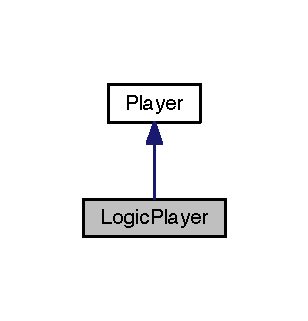
\includegraphics[width=148pt]{class_logic_player__inherit__graph}
\end{center}
\end{figure}


Collaboration diagram for Logic\+Player\+:\nopagebreak
\begin{figure}[H]
\begin{center}
\leavevmode
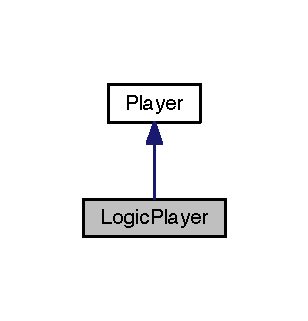
\includegraphics[width=148pt]{class_logic_player__coll__graph}
\end{center}
\end{figure}
\subsection*{Public Member Functions}
\begin{DoxyCompactItemize}
\item 
\hyperlink{class_logic_player_a9a046e3f4019b241611ba08bd9e3a2c2}{Logic\+Player} ()
\item 
\hyperlink{struct_move}{Move} \hyperlink{class_logic_player_a43a34db899e75294d73c18477c139e6a}{get\+Move} (\hyperlink{constants_8h_af901d0acc1572fb0c779f84ddd2c6ce8}{Board})
\end{DoxyCompactItemize}


\subsection{Detailed Description}


Definition at line 13 of file logic\+Player.\+h.



\subsection{Constructor \& Destructor Documentation}
\mbox{\Hypertarget{class_logic_player_a9a046e3f4019b241611ba08bd9e3a2c2}\label{class_logic_player_a9a046e3f4019b241611ba08bd9e3a2c2}} 
\index{Logic\+Player@{Logic\+Player}!Logic\+Player@{Logic\+Player}}
\index{Logic\+Player@{Logic\+Player}!Logic\+Player@{Logic\+Player}}
\subsubsection{\texorpdfstring{Logic\+Player()}{LogicPlayer()}}
{\footnotesize\ttfamily Logic\+Player\+::\+Logic\+Player (\begin{DoxyParamCaption}{ }\end{DoxyParamCaption})}



Definition at line 10 of file logic\+Player.\+cpp.



\subsection{Member Function Documentation}
\mbox{\Hypertarget{class_logic_player_a43a34db899e75294d73c18477c139e6a}\label{class_logic_player_a43a34db899e75294d73c18477c139e6a}} 
\index{Logic\+Player@{Logic\+Player}!get\+Move@{get\+Move}}
\index{get\+Move@{get\+Move}!Logic\+Player@{Logic\+Player}}
\subsubsection{\texorpdfstring{get\+Move()}{getMove()}}
{\footnotesize\ttfamily \hyperlink{struct_move}{Move} Logic\+Player\+::get\+Move (\begin{DoxyParamCaption}\item[{\hyperlink{constants_8h_af901d0acc1572fb0c779f84ddd2c6ce8}{Board}}]{board }\end{DoxyParamCaption})\hspace{0.3cm}{\ttfamily [virtual]}}



Implements \hyperlink{class_player_a97a516ce71ccef14123884b562c90e4c}{Player}.



Definition at line 13 of file logic\+Player.\+cpp.



The documentation for this class was generated from the following files\+:\begin{DoxyCompactItemize}
\item 
\hyperlink{logic_player_8h}{logic\+Player.\+h}\item 
\hyperlink{logic_player_8cpp}{logic\+Player.\+cpp}\end{DoxyCompactItemize}

\hypertarget{struct_move}{}\section{Move Struct Reference}
\label{struct_move}\index{Move@{Move}}


{\ttfamily \#include $<$constants.\+h$>$}

\subsection*{Public Member Functions}
\begin{DoxyCompactItemize}
\item 
\hyperlink{struct_move_a4b1acc3a67d30c385ad9a6000526393a}{Move} ()
\item 
\hyperlink{struct_move_aa1dd034928b13fc8a02f48bfa10f44e8}{Move} (int \hyperlink{struct_move_a078eb7da4c5a1bd0b9810453b1c25036}{row}, int \hyperlink{struct_move_a36503ec622ed1932790f7a6885ec37d3}{column}, int \hyperlink{struct_move_ad96c39b901881ab1e2e6ab59b994a815}{player})
\item 
\hyperlink{struct_move_ad8cc48006b681c9517082101d2d0c5c5}{Move} (int \hyperlink{struct_move_a078eb7da4c5a1bd0b9810453b1c25036}{row}, int col)
\end{DoxyCompactItemize}
\subsection*{Public Attributes}
\begin{DoxyCompactItemize}
\item 
int \hyperlink{struct_move_a078eb7da4c5a1bd0b9810453b1c25036}{row}
\item 
int \hyperlink{struct_move_a36503ec622ed1932790f7a6885ec37d3}{column}
\item 
int \hyperlink{struct_move_ad96c39b901881ab1e2e6ab59b994a815}{player}
\end{DoxyCompactItemize}


\subsection{Detailed Description}


Definition at line 26 of file constants.\+h.



\subsection{Constructor \& Destructor Documentation}
\mbox{\Hypertarget{struct_move_a4b1acc3a67d30c385ad9a6000526393a}\label{struct_move_a4b1acc3a67d30c385ad9a6000526393a}} 
\index{Move@{Move}!Move@{Move}}
\index{Move@{Move}!Move@{Move}}
\subsubsection{\texorpdfstring{Move()}{Move()}\hspace{0.1cm}{\footnotesize\ttfamily [1/3]}}
{\footnotesize\ttfamily Move\+::\+Move (\begin{DoxyParamCaption}{ }\end{DoxyParamCaption})\hspace{0.3cm}{\ttfamily [inline]}}



Definition at line 30 of file constants.\+h.

\mbox{\Hypertarget{struct_move_aa1dd034928b13fc8a02f48bfa10f44e8}\label{struct_move_aa1dd034928b13fc8a02f48bfa10f44e8}} 
\index{Move@{Move}!Move@{Move}}
\index{Move@{Move}!Move@{Move}}
\subsubsection{\texorpdfstring{Move()}{Move()}\hspace{0.1cm}{\footnotesize\ttfamily [2/3]}}
{\footnotesize\ttfamily Move\+::\+Move (\begin{DoxyParamCaption}\item[{int}]{row,  }\item[{int}]{column,  }\item[{int}]{player }\end{DoxyParamCaption})\hspace{0.3cm}{\ttfamily [inline]}}



Definition at line 33 of file constants.\+h.

\mbox{\Hypertarget{struct_move_ad8cc48006b681c9517082101d2d0c5c5}\label{struct_move_ad8cc48006b681c9517082101d2d0c5c5}} 
\index{Move@{Move}!Move@{Move}}
\index{Move@{Move}!Move@{Move}}
\subsubsection{\texorpdfstring{Move()}{Move()}\hspace{0.1cm}{\footnotesize\ttfamily [3/3]}}
{\footnotesize\ttfamily Move\+::\+Move (\begin{DoxyParamCaption}\item[{int}]{row,  }\item[{int}]{col }\end{DoxyParamCaption})\hspace{0.3cm}{\ttfamily [inline]}}



Definition at line 36 of file constants.\+h.



\subsection{Member Data Documentation}
\mbox{\Hypertarget{struct_move_a36503ec622ed1932790f7a6885ec37d3}\label{struct_move_a36503ec622ed1932790f7a6885ec37d3}} 
\index{Move@{Move}!column@{column}}
\index{column@{column}!Move@{Move}}
\subsubsection{\texorpdfstring{column}{column}}
{\footnotesize\ttfamily int Move\+::column}



Definition at line 27 of file constants.\+h.

\mbox{\Hypertarget{struct_move_ad96c39b901881ab1e2e6ab59b994a815}\label{struct_move_ad96c39b901881ab1e2e6ab59b994a815}} 
\index{Move@{Move}!player@{player}}
\index{player@{player}!Move@{Move}}
\subsubsection{\texorpdfstring{player}{player}}
{\footnotesize\ttfamily int Move\+::player}



Definition at line 28 of file constants.\+h.

\mbox{\Hypertarget{struct_move_a078eb7da4c5a1bd0b9810453b1c25036}\label{struct_move_a078eb7da4c5a1bd0b9810453b1c25036}} 
\index{Move@{Move}!row@{row}}
\index{row@{row}!Move@{Move}}
\subsubsection{\texorpdfstring{row}{row}}
{\footnotesize\ttfamily int Move\+::row}



Definition at line 27 of file constants.\+h.



The documentation for this struct was generated from the following file\+:\begin{DoxyCompactItemize}
\item 
\hyperlink{constants_8h}{constants.\+h}\end{DoxyCompactItemize}

\hypertarget{class_neural_network}{}\section{Neural\+Network Class Reference}
\label{class_neural_network}\index{Neural\+Network@{Neural\+Network}}


{\ttfamily \#include $<$neural\+Network.\+h$>$}



Collaboration diagram for Neural\+Network\+:\nopagebreak
\begin{figure}[H]
\begin{center}
\leavevmode
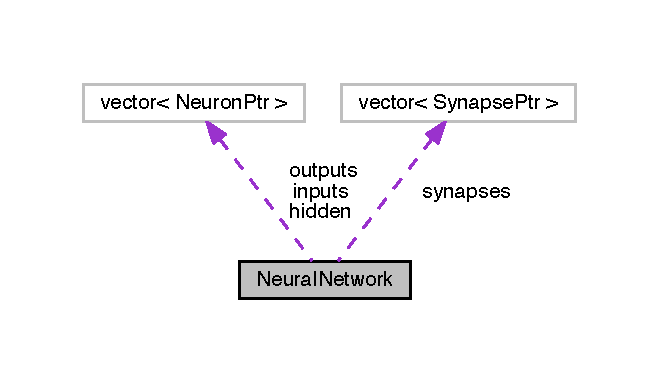
\includegraphics[width=316pt]{class_neural_network__coll__graph}
\end{center}
\end{figure}
\subsection*{Public Member Functions}
\begin{DoxyCompactItemize}
\item 
\hyperlink{class_neural_network_ac46a25af2f5a1706adf9e798970939bb}{Neural\+Network} (string s)
\item 
\hyperlink{class_neural_network_aed4b8a61c6cf3e0af6ff9976bf9c4190}{Neural\+Network} (unsigned in\+Nodes, unsigned out\+Nodes, unsigned hidden\+Nodes)
\item 
\hyperlink{class_neural_network_a4cdce541dada0debf1022e3951b8d8cb}{Neural\+Network} (unsigned in\+Nodes, unsigned out\+Nodes, unsigned layers, unsigned layer\+Nodes)
\item 
void \hyperlink{class_neural_network_adf3230528dd4c37960464557c690cbae}{save\+Network} (string s) const
\item 
void \hyperlink{class_neural_network_a7ebe119117046615958557e820b90c67}{feed\+Forward} (vector$<$ double $>$ input)
\item 
vector$<$ double $>$ \hyperlink{class_neural_network_a4416dadd62ac5ec1b645ae1378e21335}{back\+Prop} (vector$<$ vector$<$ double $>$ $>$ \hyperlink{class_neural_network_ae9ab96e97eef53bf8080001cf90075b8}{inputs}, vector$<$ vector$<$ double $>$ $>$ correct\+Outputs, vector$<$ double $>$ scaling)
\item 
vector$<$ double $>$ \hyperlink{class_neural_network_a73d030bfbf3efe8edb0bfd8a7e94ed53}{get\+Output} () const
\item 
vector$<$ double $>$ \hyperlink{class_neural_network_a7566cd3df29d6ed6d8134d2c52c1460a}{eval\+Input} (vector$<$ double $>$ input)
\item 
\hyperlink{struct_move}{Move} \hyperlink{class_neural_network_af773d118844a6dc42c8a4edc05652893}{get\+Move} (\hyperlink{constants_8h_af901d0acc1572fb0c779f84ddd2c6ce8}{Board} board)
\item 
\hyperlink{struct_move}{Move} \hyperlink{class_neural_network_abaeb2ec4b31b2a69985cacec5fd1d685}{get\+Probable\+Move} (\hyperlink{constants_8h_af901d0acc1572fb0c779f84ddd2c6ce8}{Board} board)
\end{DoxyCompactItemize}
\subsection*{Public Attributes}
\begin{DoxyCompactItemize}
\item 
vector$<$ \hyperlink{neural_network_8h_af4884b0194f2598e689c894b76d0d92c}{Neuron\+Ptr} $>$ \hyperlink{class_neural_network_ae9ab96e97eef53bf8080001cf90075b8}{inputs}
\item 
vector$<$ \hyperlink{neural_network_8h_af4884b0194f2598e689c894b76d0d92c}{Neuron\+Ptr} $>$ \hyperlink{class_neural_network_a34c4927691004c6a9a637e82f9351d28}{hidden}
\item 
vector$<$ \hyperlink{neural_network_8h_af4884b0194f2598e689c894b76d0d92c}{Neuron\+Ptr} $>$ \hyperlink{class_neural_network_aa921b31f56ca042113bf250d603dabcd}{outputs}
\item 
vector$<$ \hyperlink{neural_network_8h_ac587b5c69519c070958c5cb318ddc50f}{Synapse\+Ptr} $>$ \hyperlink{class_neural_network_aa22ab04ac7e5b3bb8f291ff524e04ee3}{synapses}
\end{DoxyCompactItemize}


\subsection{Detailed Description}


Definition at line 21 of file neural\+Network.\+h.



\subsection{Constructor \& Destructor Documentation}
\mbox{\Hypertarget{class_neural_network_ac46a25af2f5a1706adf9e798970939bb}\label{class_neural_network_ac46a25af2f5a1706adf9e798970939bb}} 
\index{Neural\+Network@{Neural\+Network}!Neural\+Network@{Neural\+Network}}
\index{Neural\+Network@{Neural\+Network}!Neural\+Network@{Neural\+Network}}
\subsubsection{\texorpdfstring{Neural\+Network()}{NeuralNetwork()}\hspace{0.1cm}{\footnotesize\ttfamily [1/3]}}
{\footnotesize\ttfamily Neural\+Network\+::\+Neural\+Network (\begin{DoxyParamCaption}\item[{string}]{s }\end{DoxyParamCaption})}



Definition at line 19 of file neural\+Network.\+cpp.

Here is the call graph for this function\+:\nopagebreak
\begin{figure}[H]
\begin{center}
\leavevmode
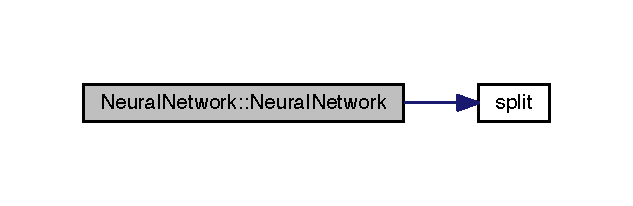
\includegraphics[width=304pt]{class_neural_network_ac46a25af2f5a1706adf9e798970939bb_cgraph}
\end{center}
\end{figure}
\mbox{\Hypertarget{class_neural_network_aed4b8a61c6cf3e0af6ff9976bf9c4190}\label{class_neural_network_aed4b8a61c6cf3e0af6ff9976bf9c4190}} 
\index{Neural\+Network@{Neural\+Network}!Neural\+Network@{Neural\+Network}}
\index{Neural\+Network@{Neural\+Network}!Neural\+Network@{Neural\+Network}}
\subsubsection{\texorpdfstring{Neural\+Network()}{NeuralNetwork()}\hspace{0.1cm}{\footnotesize\ttfamily [2/3]}}
{\footnotesize\ttfamily Neural\+Network\+::\+Neural\+Network (\begin{DoxyParamCaption}\item[{unsigned}]{in\+Nodes,  }\item[{unsigned}]{out\+Nodes,  }\item[{unsigned}]{hidden\+Nodes }\end{DoxyParamCaption})}



Definition at line 57 of file neural\+Network.\+cpp.

\mbox{\Hypertarget{class_neural_network_a4cdce541dada0debf1022e3951b8d8cb}\label{class_neural_network_a4cdce541dada0debf1022e3951b8d8cb}} 
\index{Neural\+Network@{Neural\+Network}!Neural\+Network@{Neural\+Network}}
\index{Neural\+Network@{Neural\+Network}!Neural\+Network@{Neural\+Network}}
\subsubsection{\texorpdfstring{Neural\+Network()}{NeuralNetwork()}\hspace{0.1cm}{\footnotesize\ttfamily [3/3]}}
{\footnotesize\ttfamily Neural\+Network\+::\+Neural\+Network (\begin{DoxyParamCaption}\item[{unsigned}]{in\+Nodes,  }\item[{unsigned}]{out\+Nodes,  }\item[{unsigned}]{layers,  }\item[{unsigned}]{layer\+Nodes }\end{DoxyParamCaption})}



Definition at line 87 of file neural\+Network.\+cpp.



\subsection{Member Function Documentation}
\mbox{\Hypertarget{class_neural_network_a4416dadd62ac5ec1b645ae1378e21335}\label{class_neural_network_a4416dadd62ac5ec1b645ae1378e21335}} 
\index{Neural\+Network@{Neural\+Network}!back\+Prop@{back\+Prop}}
\index{back\+Prop@{back\+Prop}!Neural\+Network@{Neural\+Network}}
\subsubsection{\texorpdfstring{back\+Prop()}{backProp()}}
{\footnotesize\ttfamily vector$<$ double $>$ Neural\+Network\+::back\+Prop (\begin{DoxyParamCaption}\item[{vector$<$ vector$<$ double $>$ $>$}]{inputs,  }\item[{vector$<$ vector$<$ double $>$ $>$}]{correct\+Outputs,  }\item[{vector$<$ double $>$}]{scaling }\end{DoxyParamCaption})}



Definition at line 163 of file neural\+Network.\+cpp.

Here is the call graph for this function\+:\nopagebreak
\begin{figure}[H]
\begin{center}
\leavevmode
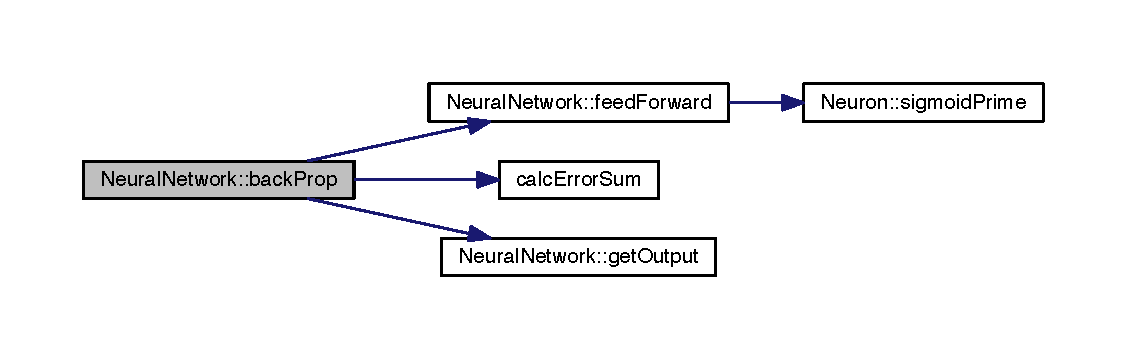
\includegraphics[width=350pt]{class_neural_network_a4416dadd62ac5ec1b645ae1378e21335_cgraph}
\end{center}
\end{figure}
\mbox{\Hypertarget{class_neural_network_a7566cd3df29d6ed6d8134d2c52c1460a}\label{class_neural_network_a7566cd3df29d6ed6d8134d2c52c1460a}} 
\index{Neural\+Network@{Neural\+Network}!eval\+Input@{eval\+Input}}
\index{eval\+Input@{eval\+Input}!Neural\+Network@{Neural\+Network}}
\subsubsection{\texorpdfstring{eval\+Input()}{evalInput()}}
{\footnotesize\ttfamily vector$<$ double $>$ Neural\+Network\+::eval\+Input (\begin{DoxyParamCaption}\item[{vector$<$ double $>$}]{input }\end{DoxyParamCaption})}



Definition at line 184 of file neural\+Network.\+cpp.

Here is the call graph for this function\+:\nopagebreak
\begin{figure}[H]
\begin{center}
\leavevmode
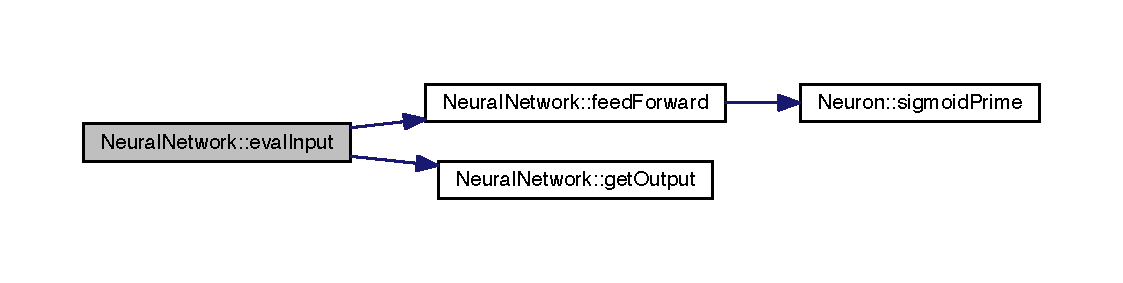
\includegraphics[width=350pt]{class_neural_network_a7566cd3df29d6ed6d8134d2c52c1460a_cgraph}
\end{center}
\end{figure}
Here is the caller graph for this function\+:\nopagebreak
\begin{figure}[H]
\begin{center}
\leavevmode
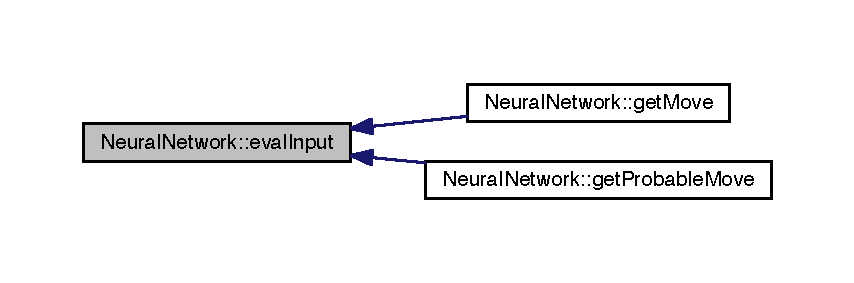
\includegraphics[width=350pt]{class_neural_network_a7566cd3df29d6ed6d8134d2c52c1460a_icgraph}
\end{center}
\end{figure}
\mbox{\Hypertarget{class_neural_network_a7ebe119117046615958557e820b90c67}\label{class_neural_network_a7ebe119117046615958557e820b90c67}} 
\index{Neural\+Network@{Neural\+Network}!feed\+Forward@{feed\+Forward}}
\index{feed\+Forward@{feed\+Forward}!Neural\+Network@{Neural\+Network}}
\subsubsection{\texorpdfstring{feed\+Forward()}{feedForward()}}
{\footnotesize\ttfamily void Neural\+Network\+::feed\+Forward (\begin{DoxyParamCaption}\item[{vector$<$ double $>$}]{input }\end{DoxyParamCaption})}



Definition at line 130 of file neural\+Network.\+cpp.

Here is the call graph for this function\+:\nopagebreak
\begin{figure}[H]
\begin{center}
\leavevmode
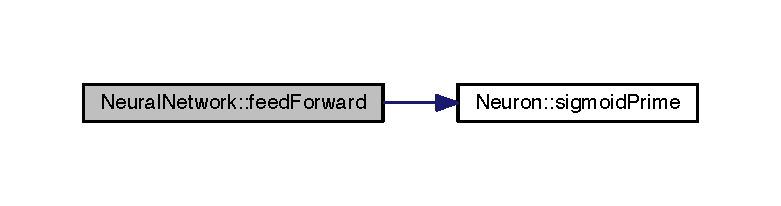
\includegraphics[width=350pt]{class_neural_network_a7ebe119117046615958557e820b90c67_cgraph}
\end{center}
\end{figure}
Here is the caller graph for this function\+:\nopagebreak
\begin{figure}[H]
\begin{center}
\leavevmode
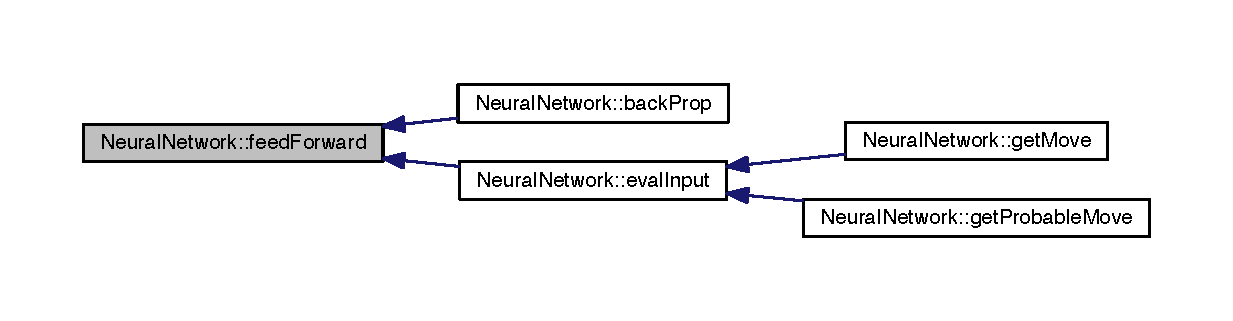
\includegraphics[width=350pt]{class_neural_network_a7ebe119117046615958557e820b90c67_icgraph}
\end{center}
\end{figure}
\mbox{\Hypertarget{class_neural_network_af773d118844a6dc42c8a4edc05652893}\label{class_neural_network_af773d118844a6dc42c8a4edc05652893}} 
\index{Neural\+Network@{Neural\+Network}!get\+Move@{get\+Move}}
\index{get\+Move@{get\+Move}!Neural\+Network@{Neural\+Network}}
\subsubsection{\texorpdfstring{get\+Move()}{getMove()}}
{\footnotesize\ttfamily \hyperlink{struct_move}{Move} Neural\+Network\+::get\+Move (\begin{DoxyParamCaption}\item[{\hyperlink{constants_8h_af901d0acc1572fb0c779f84ddd2c6ce8}{Board}}]{board }\end{DoxyParamCaption})}



Definition at line 189 of file neural\+Network.\+cpp.

Here is the call graph for this function\+:\nopagebreak
\begin{figure}[H]
\begin{center}
\leavevmode
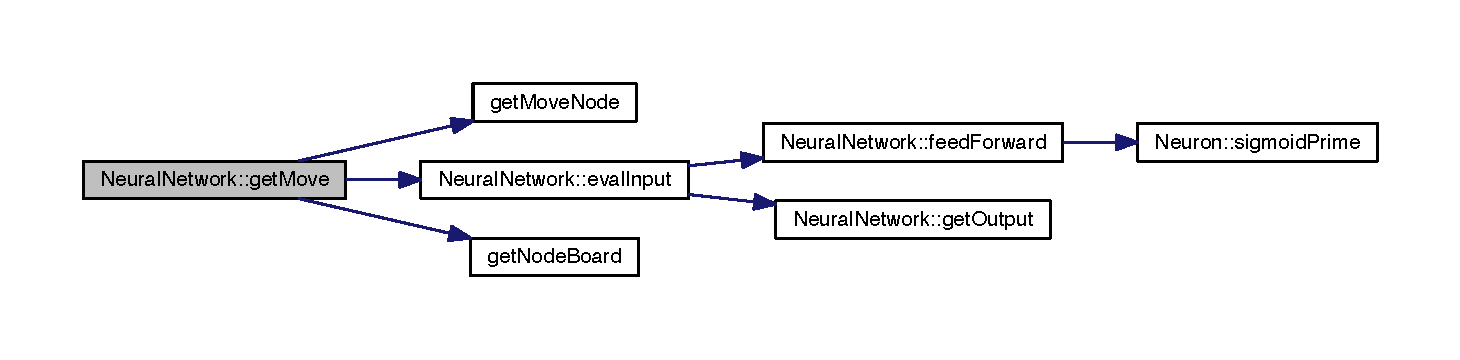
\includegraphics[width=350pt]{class_neural_network_af773d118844a6dc42c8a4edc05652893_cgraph}
\end{center}
\end{figure}
\mbox{\Hypertarget{class_neural_network_a73d030bfbf3efe8edb0bfd8a7e94ed53}\label{class_neural_network_a73d030bfbf3efe8edb0bfd8a7e94ed53}} 
\index{Neural\+Network@{Neural\+Network}!get\+Output@{get\+Output}}
\index{get\+Output@{get\+Output}!Neural\+Network@{Neural\+Network}}
\subsubsection{\texorpdfstring{get\+Output()}{getOutput()}}
{\footnotesize\ttfamily vector$<$ double $>$ Neural\+Network\+::get\+Output (\begin{DoxyParamCaption}{ }\end{DoxyParamCaption}) const}



Definition at line 197 of file neural\+Network.\+cpp.

Here is the caller graph for this function\+:\nopagebreak
\begin{figure}[H]
\begin{center}
\leavevmode
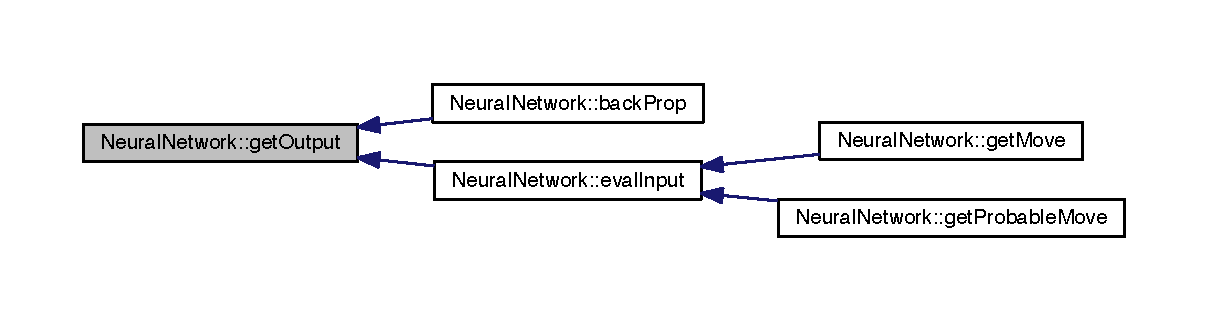
\includegraphics[width=350pt]{class_neural_network_a73d030bfbf3efe8edb0bfd8a7e94ed53_icgraph}
\end{center}
\end{figure}
\mbox{\Hypertarget{class_neural_network_abaeb2ec4b31b2a69985cacec5fd1d685}\label{class_neural_network_abaeb2ec4b31b2a69985cacec5fd1d685}} 
\index{Neural\+Network@{Neural\+Network}!get\+Probable\+Move@{get\+Probable\+Move}}
\index{get\+Probable\+Move@{get\+Probable\+Move}!Neural\+Network@{Neural\+Network}}
\subsubsection{\texorpdfstring{get\+Probable\+Move()}{getProbableMove()}}
{\footnotesize\ttfamily \hyperlink{struct_move}{Move} Neural\+Network\+::get\+Probable\+Move (\begin{DoxyParamCaption}\item[{\hyperlink{constants_8h_af901d0acc1572fb0c779f84ddd2c6ce8}{Board}}]{board }\end{DoxyParamCaption})}



Definition at line 193 of file neural\+Network.\+cpp.

Here is the call graph for this function\+:\nopagebreak
\begin{figure}[H]
\begin{center}
\leavevmode
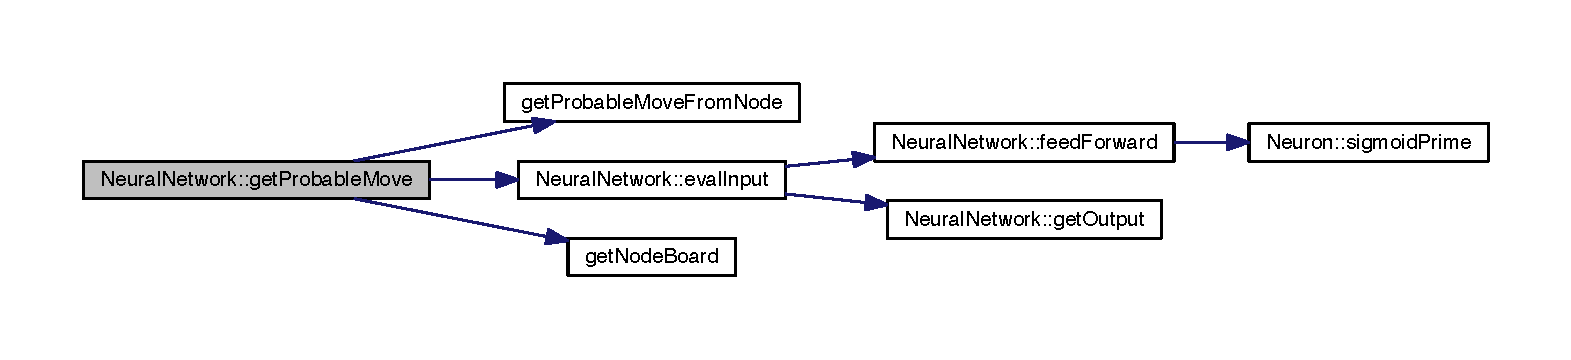
\includegraphics[width=350pt]{class_neural_network_abaeb2ec4b31b2a69985cacec5fd1d685_cgraph}
\end{center}
\end{figure}
\mbox{\Hypertarget{class_neural_network_adf3230528dd4c37960464557c690cbae}\label{class_neural_network_adf3230528dd4c37960464557c690cbae}} 
\index{Neural\+Network@{Neural\+Network}!save\+Network@{save\+Network}}
\index{save\+Network@{save\+Network}!Neural\+Network@{Neural\+Network}}
\subsubsection{\texorpdfstring{save\+Network()}{saveNetwork()}}
{\footnotesize\ttfamily void Neural\+Network\+::save\+Network (\begin{DoxyParamCaption}\item[{string}]{s }\end{DoxyParamCaption}) const}



Definition at line 205 of file neural\+Network.\+cpp.



\subsection{Member Data Documentation}
\mbox{\Hypertarget{class_neural_network_a34c4927691004c6a9a637e82f9351d28}\label{class_neural_network_a34c4927691004c6a9a637e82f9351d28}} 
\index{Neural\+Network@{Neural\+Network}!hidden@{hidden}}
\index{hidden@{hidden}!Neural\+Network@{Neural\+Network}}
\subsubsection{\texorpdfstring{hidden}{hidden}}
{\footnotesize\ttfamily vector$<$\hyperlink{neural_network_8h_af4884b0194f2598e689c894b76d0d92c}{Neuron\+Ptr}$>$ Neural\+Network\+::hidden}



Definition at line 40 of file neural\+Network.\+h.

\mbox{\Hypertarget{class_neural_network_ae9ab96e97eef53bf8080001cf90075b8}\label{class_neural_network_ae9ab96e97eef53bf8080001cf90075b8}} 
\index{Neural\+Network@{Neural\+Network}!inputs@{inputs}}
\index{inputs@{inputs}!Neural\+Network@{Neural\+Network}}
\subsubsection{\texorpdfstring{inputs}{inputs}}
{\footnotesize\ttfamily vector$<$\hyperlink{neural_network_8h_af4884b0194f2598e689c894b76d0d92c}{Neuron\+Ptr}$>$ Neural\+Network\+::inputs}



Definition at line 39 of file neural\+Network.\+h.

\mbox{\Hypertarget{class_neural_network_aa921b31f56ca042113bf250d603dabcd}\label{class_neural_network_aa921b31f56ca042113bf250d603dabcd}} 
\index{Neural\+Network@{Neural\+Network}!outputs@{outputs}}
\index{outputs@{outputs}!Neural\+Network@{Neural\+Network}}
\subsubsection{\texorpdfstring{outputs}{outputs}}
{\footnotesize\ttfamily vector$<$\hyperlink{neural_network_8h_af4884b0194f2598e689c894b76d0d92c}{Neuron\+Ptr}$>$ Neural\+Network\+::outputs}



Definition at line 41 of file neural\+Network.\+h.

\mbox{\Hypertarget{class_neural_network_aa22ab04ac7e5b3bb8f291ff524e04ee3}\label{class_neural_network_aa22ab04ac7e5b3bb8f291ff524e04ee3}} 
\index{Neural\+Network@{Neural\+Network}!synapses@{synapses}}
\index{synapses@{synapses}!Neural\+Network@{Neural\+Network}}
\subsubsection{\texorpdfstring{synapses}{synapses}}
{\footnotesize\ttfamily vector$<$\hyperlink{neural_network_8h_ac587b5c69519c070958c5cb318ddc50f}{Synapse\+Ptr}$>$ Neural\+Network\+::synapses}



Definition at line 42 of file neural\+Network.\+h.



The documentation for this class was generated from the following files\+:\begin{DoxyCompactItemize}
\item 
\hyperlink{neural_network_8h}{neural\+Network.\+h}\item 
\hyperlink{neural_network_8cpp}{neural\+Network.\+cpp}\end{DoxyCompactItemize}

\hypertarget{class_neuron}{}\section{Neuron Class Reference}
\label{class_neuron}\index{Neuron@{Neuron}}


{\ttfamily \#include $<$neuron.\+h$>$}

\subsection*{Public Member Functions}
\begin{DoxyCompactItemize}
\item 
\hyperlink{class_neuron_a823487d01615fadb8ac19a2768dd9d96}{Neuron} ()
\item 
void \hyperlink{class_neuron_a65a5533d21bd589a51a9ad502dfcb331}{feed\+Forward} ()
\item 
double \hyperlink{class_neuron_a5a84194bf3f93051d3d9f02e9146f1d4}{get\+Net\+Input} ()
\item 
double \hyperlink{class_neuron_a09bc798d5f673efd080092001ac3916c}{get\+Activity} () const
\item 
void \hyperlink{class_neuron_a53bda59e2ab1f8342a1af503a1652cdd}{set\+Activity} (double \hyperlink{class_neuron_a4f763f92e820b748629781dc8791ab9d}{activity})
\item 
const vector$<$ \hyperlink{neural_network_8h_ac587b5c69519c070958c5cb318ddc50f}{Synapse\+Ptr} $>$ \& \hyperlink{class_neuron_a976fbbfd4fa7332a412901f8f9956967}{get\+Childs} () const
\item 
void \hyperlink{class_neuron_a2960eb3ff73bd14d345f2204b2b887a4}{add\+Child} (\hyperlink{neural_network_8h_ac587b5c69519c070958c5cb318ddc50f}{Synapse\+Ptr} syn)
\item 
void \hyperlink{class_neuron_aee0e35aff21d424300a314fb0695da2e}{add\+Parent} (\hyperlink{neural_network_8h_ac587b5c69519c070958c5cb318ddc50f}{Synapse\+Ptr} syn)
\item 
unsigned \hyperlink{class_neuron_a4844d18cf096e70569b21f0e45670520}{get\+ID} () const
\end{DoxyCompactItemize}
\subsection*{Static Public Member Functions}
\begin{DoxyCompactItemize}
\item 
static double \hyperlink{class_neuron_ab151ba9bdd3e9f2aff01e782b41f92e7}{sum} (vector$<$ double $>$ x)
\item 
static double \hyperlink{class_neuron_a24893b0c92f073daae4c697b35e395f5}{sigmoid} (double x)
\item 
static double \hyperlink{class_neuron_ad2814c90d74e4400c16a116b023447fa}{sigmoid\+Prime} (double x)
\end{DoxyCompactItemize}
\subsection*{Public Attributes}
\begin{DoxyCompactItemize}
\item 
double \hyperlink{class_neuron_a4f763f92e820b748629781dc8791ab9d}{activity}
\item 
double \hyperlink{class_neuron_aa2823ed0557b8296ed5987601bad30ed}{delta}
\end{DoxyCompactItemize}


\subsection{Detailed Description}


Definition at line 17 of file neuron.\+h.



\subsection{Constructor \& Destructor Documentation}
\mbox{\Hypertarget{class_neuron_a823487d01615fadb8ac19a2768dd9d96}\label{class_neuron_a823487d01615fadb8ac19a2768dd9d96}} 
\index{Neuron@{Neuron}!Neuron@{Neuron}}
\index{Neuron@{Neuron}!Neuron@{Neuron}}
\subsubsection{\texorpdfstring{Neuron()}{Neuron()}}
{\footnotesize\ttfamily Neuron\+::\+Neuron (\begin{DoxyParamCaption}{ }\end{DoxyParamCaption})}



Definition at line 15 of file neuron.\+cpp.



\subsection{Member Function Documentation}
\mbox{\Hypertarget{class_neuron_a2960eb3ff73bd14d345f2204b2b887a4}\label{class_neuron_a2960eb3ff73bd14d345f2204b2b887a4}} 
\index{Neuron@{Neuron}!add\+Child@{add\+Child}}
\index{add\+Child@{add\+Child}!Neuron@{Neuron}}
\subsubsection{\texorpdfstring{add\+Child()}{addChild()}}
{\footnotesize\ttfamily void Neuron\+::add\+Child (\begin{DoxyParamCaption}\item[{\hyperlink{neural_network_8h_ac587b5c69519c070958c5cb318ddc50f}{Synapse\+Ptr}}]{syn }\end{DoxyParamCaption})}



Definition at line 61 of file neuron.\+cpp.

\mbox{\Hypertarget{class_neuron_aee0e35aff21d424300a314fb0695da2e}\label{class_neuron_aee0e35aff21d424300a314fb0695da2e}} 
\index{Neuron@{Neuron}!add\+Parent@{add\+Parent}}
\index{add\+Parent@{add\+Parent}!Neuron@{Neuron}}
\subsubsection{\texorpdfstring{add\+Parent()}{addParent()}}
{\footnotesize\ttfamily void Neuron\+::add\+Parent (\begin{DoxyParamCaption}\item[{\hyperlink{neural_network_8h_ac587b5c69519c070958c5cb318ddc50f}{Synapse\+Ptr}}]{syn }\end{DoxyParamCaption})}



Definition at line 65 of file neuron.\+cpp.

\mbox{\Hypertarget{class_neuron_a65a5533d21bd589a51a9ad502dfcb331}\label{class_neuron_a65a5533d21bd589a51a9ad502dfcb331}} 
\index{Neuron@{Neuron}!feed\+Forward@{feed\+Forward}}
\index{feed\+Forward@{feed\+Forward}!Neuron@{Neuron}}
\subsubsection{\texorpdfstring{feed\+Forward()}{feedForward()}}
{\footnotesize\ttfamily void Neuron\+::feed\+Forward (\begin{DoxyParamCaption}{ }\end{DoxyParamCaption})}



Definition at line 28 of file neuron.\+cpp.

Here is the call graph for this function\+:\nopagebreak
\begin{figure}[H]
\begin{center}
\leavevmode
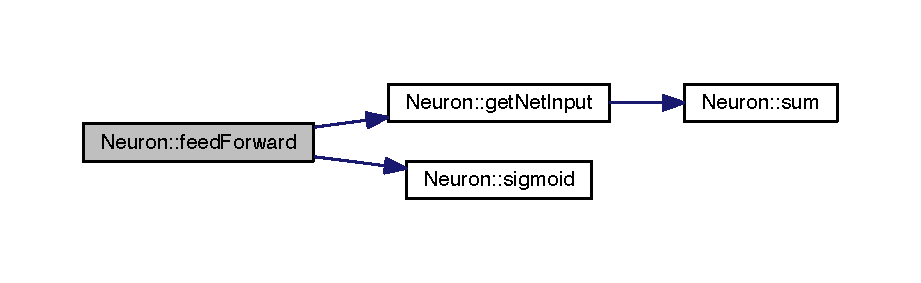
\includegraphics[width=350pt]{class_neuron_a65a5533d21bd589a51a9ad502dfcb331_cgraph}
\end{center}
\end{figure}
\mbox{\Hypertarget{class_neuron_a09bc798d5f673efd080092001ac3916c}\label{class_neuron_a09bc798d5f673efd080092001ac3916c}} 
\index{Neuron@{Neuron}!get\+Activity@{get\+Activity}}
\index{get\+Activity@{get\+Activity}!Neuron@{Neuron}}
\subsubsection{\texorpdfstring{get\+Activity()}{getActivity()}}
{\footnotesize\ttfamily double Neuron\+::get\+Activity (\begin{DoxyParamCaption}{ }\end{DoxyParamCaption}) const}



Definition at line 49 of file neuron.\+cpp.

\mbox{\Hypertarget{class_neuron_a976fbbfd4fa7332a412901f8f9956967}\label{class_neuron_a976fbbfd4fa7332a412901f8f9956967}} 
\index{Neuron@{Neuron}!get\+Childs@{get\+Childs}}
\index{get\+Childs@{get\+Childs}!Neuron@{Neuron}}
\subsubsection{\texorpdfstring{get\+Childs()}{getChilds()}}
{\footnotesize\ttfamily const vector$<$ \hyperlink{neural_network_8h_ac587b5c69519c070958c5cb318ddc50f}{Synapse\+Ptr} $>$ \& Neuron\+::get\+Childs (\begin{DoxyParamCaption}{ }\end{DoxyParamCaption}) const}



Definition at line 57 of file neuron.\+cpp.

\mbox{\Hypertarget{class_neuron_a4844d18cf096e70569b21f0e45670520}\label{class_neuron_a4844d18cf096e70569b21f0e45670520}} 
\index{Neuron@{Neuron}!get\+ID@{get\+ID}}
\index{get\+ID@{get\+ID}!Neuron@{Neuron}}
\subsubsection{\texorpdfstring{get\+I\+D()}{getID()}}
{\footnotesize\ttfamily unsigned Neuron\+::get\+ID (\begin{DoxyParamCaption}{ }\end{DoxyParamCaption}) const}



Definition at line 69 of file neuron.\+cpp.

\mbox{\Hypertarget{class_neuron_a5a84194bf3f93051d3d9f02e9146f1d4}\label{class_neuron_a5a84194bf3f93051d3d9f02e9146f1d4}} 
\index{Neuron@{Neuron}!get\+Net\+Input@{get\+Net\+Input}}
\index{get\+Net\+Input@{get\+Net\+Input}!Neuron@{Neuron}}
\subsubsection{\texorpdfstring{get\+Net\+Input()}{getNetInput()}}
{\footnotesize\ttfamily double Neuron\+::get\+Net\+Input (\begin{DoxyParamCaption}{ }\end{DoxyParamCaption})}



Definition at line 33 of file neuron.\+cpp.

Here is the call graph for this function\+:\nopagebreak
\begin{figure}[H]
\begin{center}
\leavevmode
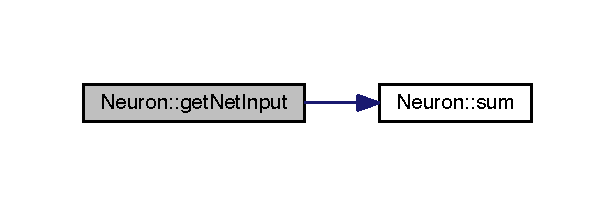
\includegraphics[width=295pt]{class_neuron_a5a84194bf3f93051d3d9f02e9146f1d4_cgraph}
\end{center}
\end{figure}
Here is the caller graph for this function\+:\nopagebreak
\begin{figure}[H]
\begin{center}
\leavevmode
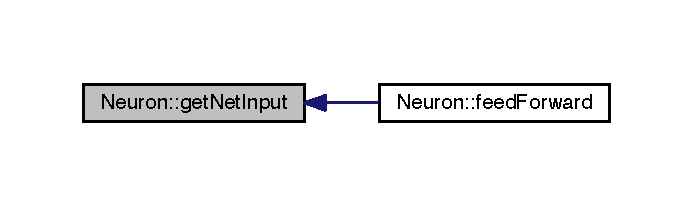
\includegraphics[width=333pt]{class_neuron_a5a84194bf3f93051d3d9f02e9146f1d4_icgraph}
\end{center}
\end{figure}
\mbox{\Hypertarget{class_neuron_a53bda59e2ab1f8342a1af503a1652cdd}\label{class_neuron_a53bda59e2ab1f8342a1af503a1652cdd}} 
\index{Neuron@{Neuron}!set\+Activity@{set\+Activity}}
\index{set\+Activity@{set\+Activity}!Neuron@{Neuron}}
\subsubsection{\texorpdfstring{set\+Activity()}{setActivity()}}
{\footnotesize\ttfamily void Neuron\+::set\+Activity (\begin{DoxyParamCaption}\item[{double}]{activity }\end{DoxyParamCaption})}



Definition at line 53 of file neuron.\+cpp.

\mbox{\Hypertarget{class_neuron_a24893b0c92f073daae4c697b35e395f5}\label{class_neuron_a24893b0c92f073daae4c697b35e395f5}} 
\index{Neuron@{Neuron}!sigmoid@{sigmoid}}
\index{sigmoid@{sigmoid}!Neuron@{Neuron}}
\subsubsection{\texorpdfstring{sigmoid()}{sigmoid()}}
{\footnotesize\ttfamily double Neuron\+::sigmoid (\begin{DoxyParamCaption}\item[{double}]{x }\end{DoxyParamCaption})\hspace{0.3cm}{\ttfamily [static]}}



Definition at line 41 of file neuron.\+cpp.

Here is the caller graph for this function\+:\nopagebreak
\begin{figure}[H]
\begin{center}
\leavevmode
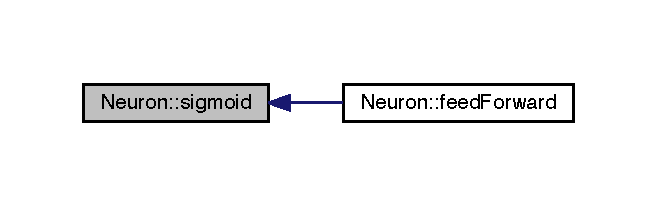
\includegraphics[width=315pt]{class_neuron_a24893b0c92f073daae4c697b35e395f5_icgraph}
\end{center}
\end{figure}
\mbox{\Hypertarget{class_neuron_ad2814c90d74e4400c16a116b023447fa}\label{class_neuron_ad2814c90d74e4400c16a116b023447fa}} 
\index{Neuron@{Neuron}!sigmoid\+Prime@{sigmoid\+Prime}}
\index{sigmoid\+Prime@{sigmoid\+Prime}!Neuron@{Neuron}}
\subsubsection{\texorpdfstring{sigmoid\+Prime()}{sigmoidPrime()}}
{\footnotesize\ttfamily double Neuron\+::sigmoid\+Prime (\begin{DoxyParamCaption}\item[{double}]{x }\end{DoxyParamCaption})\hspace{0.3cm}{\ttfamily [static]}}



Definition at line 45 of file neuron.\+cpp.

Here is the caller graph for this function\+:\nopagebreak
\begin{figure}[H]
\begin{center}
\leavevmode
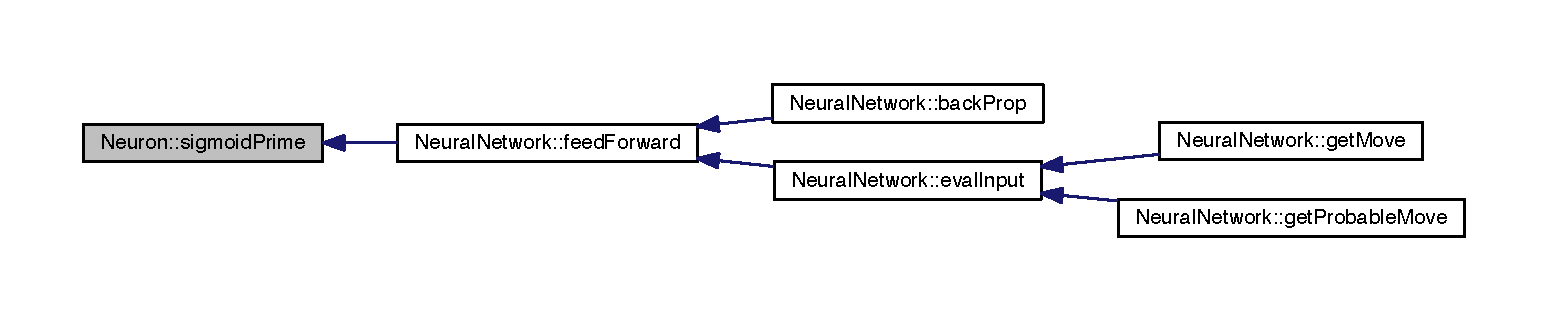
\includegraphics[width=350pt]{class_neuron_ad2814c90d74e4400c16a116b023447fa_icgraph}
\end{center}
\end{figure}
\mbox{\Hypertarget{class_neuron_ab151ba9bdd3e9f2aff01e782b41f92e7}\label{class_neuron_ab151ba9bdd3e9f2aff01e782b41f92e7}} 
\index{Neuron@{Neuron}!sum@{sum}}
\index{sum@{sum}!Neuron@{Neuron}}
\subsubsection{\texorpdfstring{sum()}{sum()}}
{\footnotesize\ttfamily double Neuron\+::sum (\begin{DoxyParamCaption}\item[{vector$<$ double $>$}]{x }\end{DoxyParamCaption})\hspace{0.3cm}{\ttfamily [static]}}



Definition at line 20 of file neuron.\+cpp.

Here is the caller graph for this function\+:\nopagebreak
\begin{figure}[H]
\begin{center}
\leavevmode
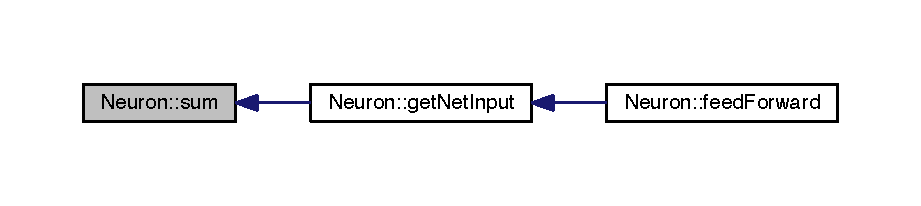
\includegraphics[width=350pt]{class_neuron_ab151ba9bdd3e9f2aff01e782b41f92e7_icgraph}
\end{center}
\end{figure}


\subsection{Member Data Documentation}
\mbox{\Hypertarget{class_neuron_a4f763f92e820b748629781dc8791ab9d}\label{class_neuron_a4f763f92e820b748629781dc8791ab9d}} 
\index{Neuron@{Neuron}!activity@{activity}}
\index{activity@{activity}!Neuron@{Neuron}}
\subsubsection{\texorpdfstring{activity}{activity}}
{\footnotesize\ttfamily double Neuron\+::activity}



Definition at line 36 of file neuron.\+h.

\mbox{\Hypertarget{class_neuron_aa2823ed0557b8296ed5987601bad30ed}\label{class_neuron_aa2823ed0557b8296ed5987601bad30ed}} 
\index{Neuron@{Neuron}!delta@{delta}}
\index{delta@{delta}!Neuron@{Neuron}}
\subsubsection{\texorpdfstring{delta}{delta}}
{\footnotesize\ttfamily double Neuron\+::delta}



Definition at line 37 of file neuron.\+h.



The documentation for this class was generated from the following files\+:\begin{DoxyCompactItemize}
\item 
\hyperlink{neuron_8h}{neuron.\+h}\item 
\hyperlink{neuron_8cpp}{neuron.\+cpp}\end{DoxyCompactItemize}

\hypertarget{class_player}{}\section{Player Class Reference}
\label{class_player}\index{Player@{Player}}


{\ttfamily \#include $<$player.\+h$>$}



Inheritance diagram for Player\+:\nopagebreak
\begin{figure}[H]
\begin{center}
\leavevmode
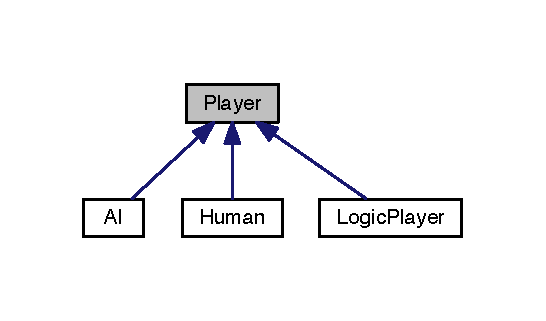
\includegraphics[width=262pt]{class_player__inherit__graph}
\end{center}
\end{figure}
\subsection*{Public Member Functions}
\begin{DoxyCompactItemize}
\item 
\hyperlink{class_player_affe0cc3cb714f6deb4e62f0c0d3f1fd8}{Player} ()
\item 
virtual \hyperlink{class_player_a749d2c00e1fe0f5c2746f7505a58c062}{$\sim$\+Player} ()
\item 
virtual \hyperlink{struct_move}{Move} \hyperlink{class_player_a97a516ce71ccef14123884b562c90e4c}{get\+Move} (\hyperlink{constants_8h_af901d0acc1572fb0c779f84ddd2c6ce8}{Board})=0
\end{DoxyCompactItemize}


\subsection{Detailed Description}


Definition at line 13 of file player.\+h.



\subsection{Constructor \& Destructor Documentation}
\mbox{\Hypertarget{class_player_affe0cc3cb714f6deb4e62f0c0d3f1fd8}\label{class_player_affe0cc3cb714f6deb4e62f0c0d3f1fd8}} 
\index{Player@{Player}!Player@{Player}}
\index{Player@{Player}!Player@{Player}}
\subsubsection{\texorpdfstring{Player()}{Player()}}
{\footnotesize\ttfamily Player\+::\+Player (\begin{DoxyParamCaption}{ }\end{DoxyParamCaption})}



Definition at line 10 of file player.\+cpp.

\mbox{\Hypertarget{class_player_a749d2c00e1fe0f5c2746f7505a58c062}\label{class_player_a749d2c00e1fe0f5c2746f7505a58c062}} 
\index{Player@{Player}!````~Player@{$\sim$\+Player}}
\index{````~Player@{$\sim$\+Player}!Player@{Player}}
\subsubsection{\texorpdfstring{$\sim$\+Player()}{~Player()}}
{\footnotesize\ttfamily Player\+::$\sim$\+Player (\begin{DoxyParamCaption}{ }\end{DoxyParamCaption})\hspace{0.3cm}{\ttfamily [virtual]}}



Definition at line 13 of file player.\+cpp.



\subsection{Member Function Documentation}
\mbox{\Hypertarget{class_player_a97a516ce71ccef14123884b562c90e4c}\label{class_player_a97a516ce71ccef14123884b562c90e4c}} 
\index{Player@{Player}!get\+Move@{get\+Move}}
\index{get\+Move@{get\+Move}!Player@{Player}}
\subsubsection{\texorpdfstring{get\+Move()}{getMove()}}
{\footnotesize\ttfamily virtual \hyperlink{struct_move}{Move} Player\+::get\+Move (\begin{DoxyParamCaption}\item[{\hyperlink{constants_8h_af901d0acc1572fb0c779f84ddd2c6ce8}{Board}}]{ }\end{DoxyParamCaption})\hspace{0.3cm}{\ttfamily [pure virtual]}}



Implemented in \hyperlink{class_a_i_a2d1a6ed520e3b3ada7133bd03d405d6d}{AI}, \hyperlink{class_human_a61228d0fbea51c587ea5383d84b152d8}{Human}, and \hyperlink{class_logic_player_a43a34db899e75294d73c18477c139e6a}{Logic\+Player}.



The documentation for this class was generated from the following files\+:\begin{DoxyCompactItemize}
\item 
\hyperlink{player_8h}{player.\+h}\item 
\hyperlink{player_8cpp}{player.\+cpp}\end{DoxyCompactItemize}

\hypertarget{class_runner}{}\section{Runner Class Reference}
\label{class_runner}\index{Runner@{Runner}}


{\ttfamily \#include $<$runner.\+h$>$}

\subsection*{Public Member Functions}
\begin{DoxyCompactItemize}
\item 
\hyperlink{class_runner_a4bcd8507e4e2e5a1f06d056bd5170144}{Runner} (\hyperlink{runner_8h_afe5d34ded509e15b538d78ebe5cb3db6}{Player\+Ptr}, \hyperlink{runner_8h_afe5d34ded509e15b538d78ebe5cb3db6}{Player\+Ptr})
\item 
bool \hyperlink{class_runner_aa3c82c871ab414550822f993efad22a5}{is\+Draw} () const
\item 
int \hyperlink{class_runner_aa4e55d3ecb77ffc83dfde5dc1fc3663b}{get\+Winner} () const
\item 
vector$<$ \hyperlink{constants_8h_afd2599a4148deb913a46b4e2eba9e68a}{State} $>$ \hyperlink{class_runner_ae3105a026f21ed05a8c022857cd12617}{get\+Bad\+States} () const
\item 
vector$<$ \hyperlink{constants_8h_afd2599a4148deb913a46b4e2eba9e68a}{State} $>$ \hyperlink{class_runner_a2d1297463b5825f5afa1e3e502919698}{get\+Good\+States} () const
\item 
const vector$<$ \hyperlink{struct_move}{Move} $>$ \& \hyperlink{class_runner_aebd1690762a996fbad5aa1b56d3aacc0}{get\+Moves} () const
\item 
void \hyperlink{class_runner_a4cc0bf3493f80516761032d55cc2ffab}{dump} () const
\end{DoxyCompactItemize}


\subsection{Detailed Description}


Definition at line 13 of file runner.\+h.



\subsection{Constructor \& Destructor Documentation}
\mbox{\Hypertarget{class_runner_a4bcd8507e4e2e5a1f06d056bd5170144}\label{class_runner_a4bcd8507e4e2e5a1f06d056bd5170144}} 
\index{Runner@{Runner}!Runner@{Runner}}
\index{Runner@{Runner}!Runner@{Runner}}
\subsubsection{\texorpdfstring{Runner()}{Runner()}}
{\footnotesize\ttfamily Runner\+::\+Runner (\begin{DoxyParamCaption}\item[{\hyperlink{runner_8h_afe5d34ded509e15b538d78ebe5cb3db6}{Player\+Ptr}}]{player1,  }\item[{\hyperlink{runner_8h_afe5d34ded509e15b538d78ebe5cb3db6}{Player\+Ptr}}]{player2 }\end{DoxyParamCaption})}



Definition at line 6 of file runner.\+cpp.



\subsection{Member Function Documentation}
\mbox{\Hypertarget{class_runner_a4cc0bf3493f80516761032d55cc2ffab}\label{class_runner_a4cc0bf3493f80516761032d55cc2ffab}} 
\index{Runner@{Runner}!dump@{dump}}
\index{dump@{dump}!Runner@{Runner}}
\subsubsection{\texorpdfstring{dump()}{dump()}}
{\footnotesize\ttfamily void Runner\+::dump (\begin{DoxyParamCaption}{ }\end{DoxyParamCaption}) const}



Definition at line 19 of file runner.\+cpp.

Here is the call graph for this function\+:\nopagebreak
\begin{figure}[H]
\begin{center}
\leavevmode
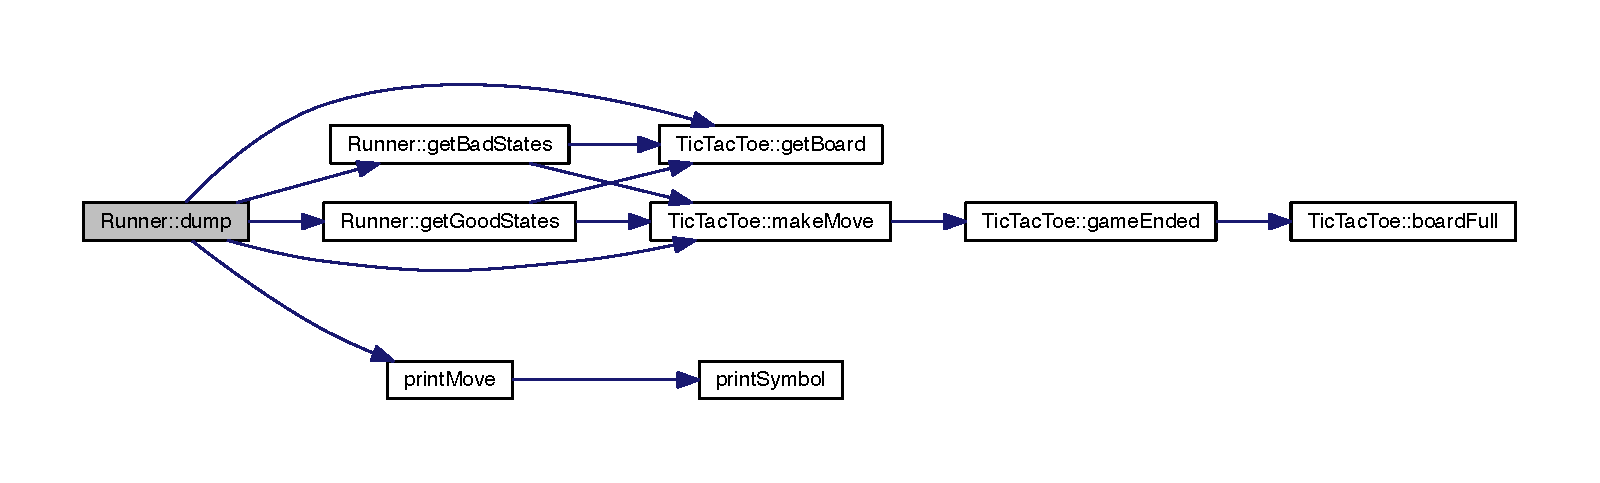
\includegraphics[width=350pt]{class_runner_a4cc0bf3493f80516761032d55cc2ffab_cgraph}
\end{center}
\end{figure}
Here is the caller graph for this function\+:\nopagebreak
\begin{figure}[H]
\begin{center}
\leavevmode
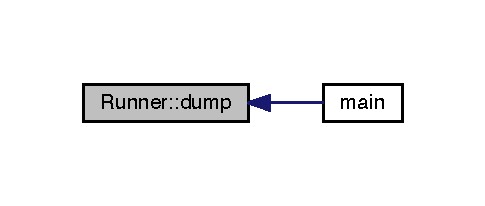
\includegraphics[width=233pt]{class_runner_a4cc0bf3493f80516761032d55cc2ffab_icgraph}
\end{center}
\end{figure}
\mbox{\Hypertarget{class_runner_ae3105a026f21ed05a8c022857cd12617}\label{class_runner_ae3105a026f21ed05a8c022857cd12617}} 
\index{Runner@{Runner}!get\+Bad\+States@{get\+Bad\+States}}
\index{get\+Bad\+States@{get\+Bad\+States}!Runner@{Runner}}
\subsubsection{\texorpdfstring{get\+Bad\+States()}{getBadStates()}}
{\footnotesize\ttfamily vector$<$ \hyperlink{constants_8h_afd2599a4148deb913a46b4e2eba9e68a}{State} $>$ Runner\+::get\+Bad\+States (\begin{DoxyParamCaption}{ }\end{DoxyParamCaption}) const}



Definition at line 65 of file runner.\+cpp.

Here is the call graph for this function\+:\nopagebreak
\begin{figure}[H]
\begin{center}
\leavevmode
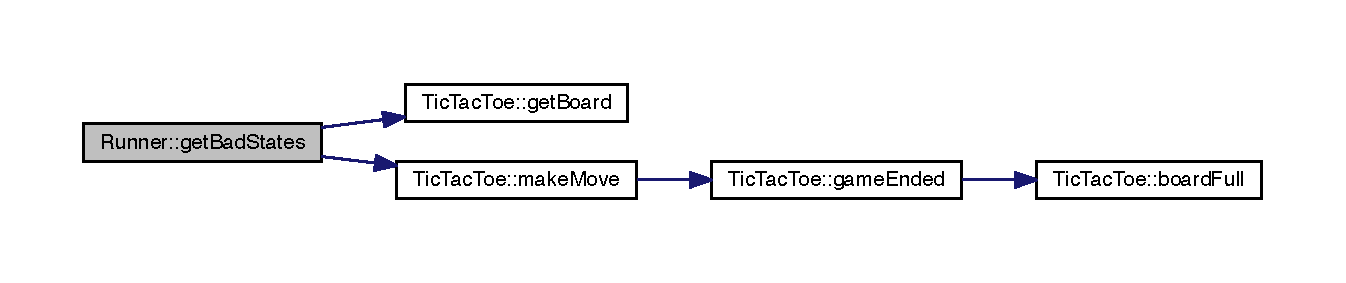
\includegraphics[width=350pt]{class_runner_ae3105a026f21ed05a8c022857cd12617_cgraph}
\end{center}
\end{figure}
Here is the caller graph for this function\+:\nopagebreak
\begin{figure}[H]
\begin{center}
\leavevmode
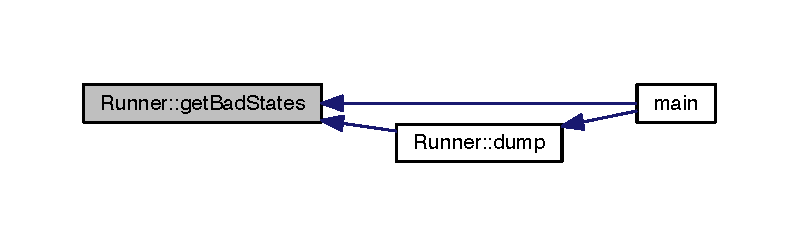
\includegraphics[width=350pt]{class_runner_ae3105a026f21ed05a8c022857cd12617_icgraph}
\end{center}
\end{figure}
\mbox{\Hypertarget{class_runner_a2d1297463b5825f5afa1e3e502919698}\label{class_runner_a2d1297463b5825f5afa1e3e502919698}} 
\index{Runner@{Runner}!get\+Good\+States@{get\+Good\+States}}
\index{get\+Good\+States@{get\+Good\+States}!Runner@{Runner}}
\subsubsection{\texorpdfstring{get\+Good\+States()}{getGoodStates()}}
{\footnotesize\ttfamily vector$<$ \hyperlink{constants_8h_afd2599a4148deb913a46b4e2eba9e68a}{State} $>$ Runner\+::get\+Good\+States (\begin{DoxyParamCaption}{ }\end{DoxyParamCaption}) const}



Definition at line 50 of file runner.\+cpp.

Here is the call graph for this function\+:\nopagebreak
\begin{figure}[H]
\begin{center}
\leavevmode
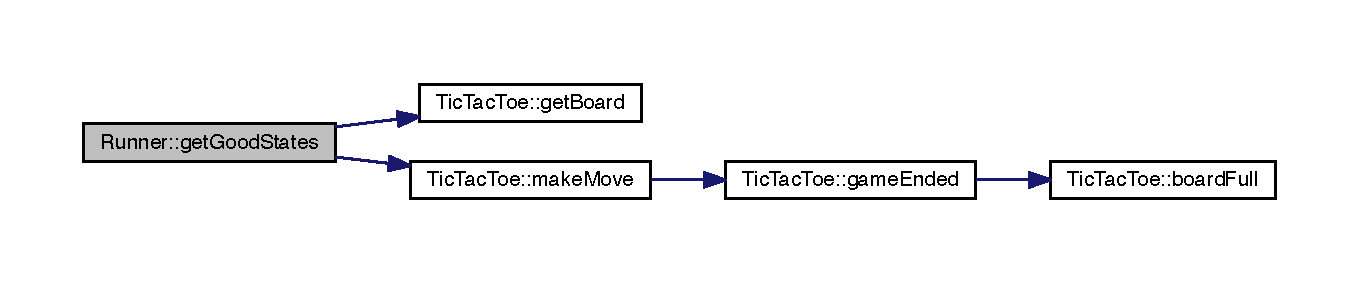
\includegraphics[width=350pt]{class_runner_a2d1297463b5825f5afa1e3e502919698_cgraph}
\end{center}
\end{figure}
Here is the caller graph for this function\+:\nopagebreak
\begin{figure}[H]
\begin{center}
\leavevmode
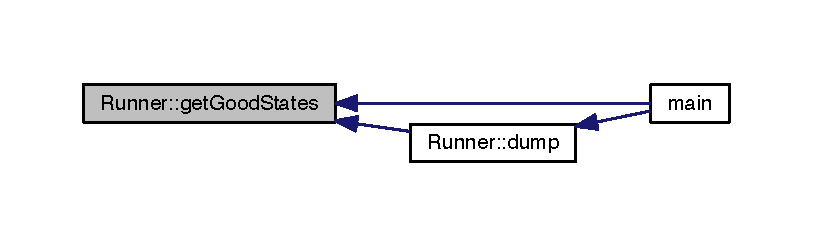
\includegraphics[width=350pt]{class_runner_a2d1297463b5825f5afa1e3e502919698_icgraph}
\end{center}
\end{figure}
\mbox{\Hypertarget{class_runner_aebd1690762a996fbad5aa1b56d3aacc0}\label{class_runner_aebd1690762a996fbad5aa1b56d3aacc0}} 
\index{Runner@{Runner}!get\+Moves@{get\+Moves}}
\index{get\+Moves@{get\+Moves}!Runner@{Runner}}
\subsubsection{\texorpdfstring{get\+Moves()}{getMoves()}}
{\footnotesize\ttfamily const vector$<$ \hyperlink{struct_move}{Move} $>$ \& Runner\+::get\+Moves (\begin{DoxyParamCaption}{ }\end{DoxyParamCaption}) const}



Definition at line 80 of file runner.\+cpp.

Here is the caller graph for this function\+:\nopagebreak
\begin{figure}[H]
\begin{center}
\leavevmode
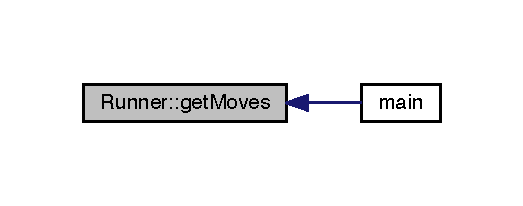
\includegraphics[width=251pt]{class_runner_aebd1690762a996fbad5aa1b56d3aacc0_icgraph}
\end{center}
\end{figure}
\mbox{\Hypertarget{class_runner_aa4e55d3ecb77ffc83dfde5dc1fc3663b}\label{class_runner_aa4e55d3ecb77ffc83dfde5dc1fc3663b}} 
\index{Runner@{Runner}!get\+Winner@{get\+Winner}}
\index{get\+Winner@{get\+Winner}!Runner@{Runner}}
\subsubsection{\texorpdfstring{get\+Winner()}{getWinner()}}
{\footnotesize\ttfamily int Runner\+::get\+Winner (\begin{DoxyParamCaption}{ }\end{DoxyParamCaption}) const}



Definition at line 15 of file runner.\+cpp.

Here is the caller graph for this function\+:\nopagebreak
\begin{figure}[H]
\begin{center}
\leavevmode
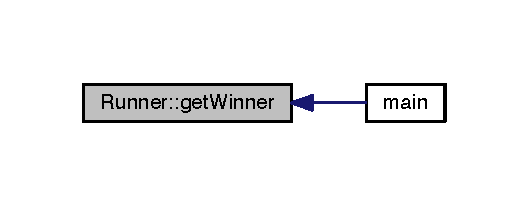
\includegraphics[width=254pt]{class_runner_aa4e55d3ecb77ffc83dfde5dc1fc3663b_icgraph}
\end{center}
\end{figure}
\mbox{\Hypertarget{class_runner_aa3c82c871ab414550822f993efad22a5}\label{class_runner_aa3c82c871ab414550822f993efad22a5}} 
\index{Runner@{Runner}!is\+Draw@{is\+Draw}}
\index{is\+Draw@{is\+Draw}!Runner@{Runner}}
\subsubsection{\texorpdfstring{is\+Draw()}{isDraw()}}
{\footnotesize\ttfamily bool Runner\+::is\+Draw (\begin{DoxyParamCaption}{ }\end{DoxyParamCaption}) const}



Definition at line 11 of file runner.\+cpp.

Here is the caller graph for this function\+:\nopagebreak
\begin{figure}[H]
\begin{center}
\leavevmode
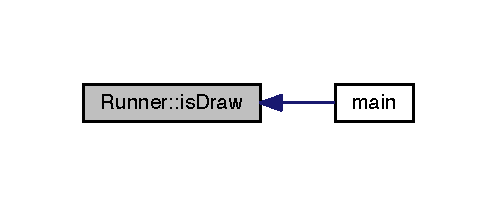
\includegraphics[width=239pt]{class_runner_aa3c82c871ab414550822f993efad22a5_icgraph}
\end{center}
\end{figure}


The documentation for this class was generated from the following files\+:\begin{DoxyCompactItemize}
\item 
\hyperlink{runner_8h}{runner.\+h}\item 
\hyperlink{runner_8cpp}{runner.\+cpp}\end{DoxyCompactItemize}

\hypertarget{class_synapse}{}\section{Synapse Class Reference}
\label{class_synapse}\index{Synapse@{Synapse}}


{\ttfamily \#include $<$synapse.\+h$>$}

\subsection*{Public Member Functions}
\begin{DoxyCompactItemize}
\item 
\hyperlink{class_synapse_ad7d17e64c370f530debc6755ff39c866}{Synapse} (\hyperlink{neural_network_8h_af4884b0194f2598e689c894b76d0d92c}{Neuron\+Ptr} in, \hyperlink{neural_network_8h_af4884b0194f2598e689c894b76d0d92c}{Neuron\+Ptr} out)
\item 
double \hyperlink{class_synapse_af46174272161c65aa44279c92f8e625b}{get\+Signal} ()
\item 
const \hyperlink{neural_network_8h_af4884b0194f2598e689c894b76d0d92c}{Neuron\+Ptr} \hyperlink{class_synapse_ac6f0d40b4c56391f6eaf17c062112089}{get\+In} () const
\item 
const \hyperlink{neural_network_8h_af4884b0194f2598e689c894b76d0d92c}{Neuron\+Ptr} \hyperlink{class_synapse_a98bb7ae4e2b75edfd07f1366cba6cc80}{get\+Out} () const
\item 
unsigned \hyperlink{class_synapse_a82879d96c983b1a788c69f8144bd3095}{get\+ID} () const
\end{DoxyCompactItemize}
\subsection*{Public Attributes}
\begin{DoxyCompactItemize}
\item 
double \hyperlink{class_synapse_a44d98296097d0130667a45ee2645fe2b}{weight}
\item 
double \hyperlink{class_synapse_a6346dada19b7ff4cd5a20764e07665c3}{weight\+Change}
\end{DoxyCompactItemize}
\subsection*{Static Public Attributes}
\begin{DoxyCompactItemize}
\item 
static double \hyperlink{class_synapse_a1ea4d11c389bcf1e090c5f74c7c3f9ac}{learning\+Rate} = 0.\+2
\end{DoxyCompactItemize}


\subsection{Detailed Description}


Definition at line 16 of file synapse.\+h.



\subsection{Constructor \& Destructor Documentation}
\mbox{\Hypertarget{class_synapse_ad7d17e64c370f530debc6755ff39c866}\label{class_synapse_ad7d17e64c370f530debc6755ff39c866}} 
\index{Synapse@{Synapse}!Synapse@{Synapse}}
\index{Synapse@{Synapse}!Synapse@{Synapse}}
\subsubsection{\texorpdfstring{Synapse()}{Synapse()}}
{\footnotesize\ttfamily Synapse\+::\+Synapse (\begin{DoxyParamCaption}\item[{\hyperlink{neural_network_8h_af4884b0194f2598e689c894b76d0d92c}{Neuron\+Ptr}}]{in,  }\item[{\hyperlink{neural_network_8h_af4884b0194f2598e689c894b76d0d92c}{Neuron\+Ptr}}]{out }\end{DoxyParamCaption})}



Definition at line 16 of file synapse.\+cpp.



\subsection{Member Function Documentation}
\mbox{\Hypertarget{class_synapse_a82879d96c983b1a788c69f8144bd3095}\label{class_synapse_a82879d96c983b1a788c69f8144bd3095}} 
\index{Synapse@{Synapse}!get\+ID@{get\+ID}}
\index{get\+ID@{get\+ID}!Synapse@{Synapse}}
\subsubsection{\texorpdfstring{get\+I\+D()}{getID()}}
{\footnotesize\ttfamily unsigned Synapse\+::get\+ID (\begin{DoxyParamCaption}{ }\end{DoxyParamCaption}) const\hspace{0.3cm}{\ttfamily [inline]}}



Definition at line 30 of file synapse.\+h.

\mbox{\Hypertarget{class_synapse_ac6f0d40b4c56391f6eaf17c062112089}\label{class_synapse_ac6f0d40b4c56391f6eaf17c062112089}} 
\index{Synapse@{Synapse}!get\+In@{get\+In}}
\index{get\+In@{get\+In}!Synapse@{Synapse}}
\subsubsection{\texorpdfstring{get\+In()}{getIn()}}
{\footnotesize\ttfamily const \hyperlink{neural_network_8h_af4884b0194f2598e689c894b76d0d92c}{Neuron\+Ptr} Synapse\+::get\+In (\begin{DoxyParamCaption}{ }\end{DoxyParamCaption}) const\hspace{0.3cm}{\ttfamily [inline]}}



Definition at line 22 of file synapse.\+h.

\mbox{\Hypertarget{class_synapse_a98bb7ae4e2b75edfd07f1366cba6cc80}\label{class_synapse_a98bb7ae4e2b75edfd07f1366cba6cc80}} 
\index{Synapse@{Synapse}!get\+Out@{get\+Out}}
\index{get\+Out@{get\+Out}!Synapse@{Synapse}}
\subsubsection{\texorpdfstring{get\+Out()}{getOut()}}
{\footnotesize\ttfamily const \hyperlink{neural_network_8h_af4884b0194f2598e689c894b76d0d92c}{Neuron\+Ptr} Synapse\+::get\+Out (\begin{DoxyParamCaption}{ }\end{DoxyParamCaption}) const\hspace{0.3cm}{\ttfamily [inline]}}



Definition at line 26 of file synapse.\+h.

\mbox{\Hypertarget{class_synapse_af46174272161c65aa44279c92f8e625b}\label{class_synapse_af46174272161c65aa44279c92f8e625b}} 
\index{Synapse@{Synapse}!get\+Signal@{get\+Signal}}
\index{get\+Signal@{get\+Signal}!Synapse@{Synapse}}
\subsubsection{\texorpdfstring{get\+Signal()}{getSignal()}}
{\footnotesize\ttfamily double Synapse\+::get\+Signal (\begin{DoxyParamCaption}{ }\end{DoxyParamCaption})}



Definition at line 26 of file synapse.\+cpp.



\subsection{Member Data Documentation}
\mbox{\Hypertarget{class_synapse_a1ea4d11c389bcf1e090c5f74c7c3f9ac}\label{class_synapse_a1ea4d11c389bcf1e090c5f74c7c3f9ac}} 
\index{Synapse@{Synapse}!learning\+Rate@{learning\+Rate}}
\index{learning\+Rate@{learning\+Rate}!Synapse@{Synapse}}
\subsubsection{\texorpdfstring{learning\+Rate}{learningRate}}
{\footnotesize\ttfamily double Synapse\+::learning\+Rate = 0.\+2\hspace{0.3cm}{\ttfamily [static]}}



Definition at line 36 of file synapse.\+h.

\mbox{\Hypertarget{class_synapse_a44d98296097d0130667a45ee2645fe2b}\label{class_synapse_a44d98296097d0130667a45ee2645fe2b}} 
\index{Synapse@{Synapse}!weight@{weight}}
\index{weight@{weight}!Synapse@{Synapse}}
\subsubsection{\texorpdfstring{weight}{weight}}
{\footnotesize\ttfamily double Synapse\+::weight}



Definition at line 34 of file synapse.\+h.

\mbox{\Hypertarget{class_synapse_a6346dada19b7ff4cd5a20764e07665c3}\label{class_synapse_a6346dada19b7ff4cd5a20764e07665c3}} 
\index{Synapse@{Synapse}!weight\+Change@{weight\+Change}}
\index{weight\+Change@{weight\+Change}!Synapse@{Synapse}}
\subsubsection{\texorpdfstring{weight\+Change}{weightChange}}
{\footnotesize\ttfamily double Synapse\+::weight\+Change}



Definition at line 35 of file synapse.\+h.



The documentation for this class was generated from the following files\+:\begin{DoxyCompactItemize}
\item 
\hyperlink{synapse_8h}{synapse.\+h}\item 
\hyperlink{synapse_8cpp}{synapse.\+cpp}\end{DoxyCompactItemize}

\hypertarget{class_tic_tac_toe}{}\section{Tic\+Tac\+Toe Class Reference}
\label{class_tic_tac_toe}\index{Tic\+Tac\+Toe@{Tic\+Tac\+Toe}}


The game \hyperlink{class_tic_tac_toe}{Tic\+Tac\+Toe}.  




{\ttfamily \#include $<$tictactoe.\+h$>$}

\subsection*{Public Member Functions}
\begin{DoxyCompactItemize}
\item 
\hyperlink{class_tic_tac_toe_a103fe9a5ae41b5ef756e20594a70cb7a}{Tic\+Tac\+Toe} ()
\item 
int \hyperlink{class_tic_tac_toe_a597a1911309c9350aa6ce48b817a0e9e}{make\+Move} (int row, int column, int player)
\item 
\hyperlink{constants_8h_af901d0acc1572fb0c779f84ddd2c6ce8}{Board} \hyperlink{class_tic_tac_toe_aeacd5865fa7f87f6fd9608b8ed1743a9}{get\+Board} (int player)
\item 
int \hyperlink{class_tic_tac_toe_a0ed1b3b4b699af8e7db79f502cbc9531}{game\+Ended} ()
\item 
bool \hyperlink{class_tic_tac_toe_a750e26d95ced2dca83c21279ef43def9}{board\+Full} ()
\end{DoxyCompactItemize}


\subsection{Detailed Description}
The game \hyperlink{class_tic_tac_toe}{Tic\+Tac\+Toe}. 

This class represents a playable game of \hyperlink{class_tic_tac_toe}{Tic\+Tac\+Toe}. 

Definition at line 11 of file tictactoe.\+h.



\subsection{Constructor \& Destructor Documentation}
\mbox{\Hypertarget{class_tic_tac_toe_a103fe9a5ae41b5ef756e20594a70cb7a}\label{class_tic_tac_toe_a103fe9a5ae41b5ef756e20594a70cb7a}} 
\index{Tic\+Tac\+Toe@{Tic\+Tac\+Toe}!Tic\+Tac\+Toe@{Tic\+Tac\+Toe}}
\index{Tic\+Tac\+Toe@{Tic\+Tac\+Toe}!Tic\+Tac\+Toe@{Tic\+Tac\+Toe}}
\subsubsection{\texorpdfstring{Tic\+Tac\+Toe()}{TicTacToe()}}
{\footnotesize\ttfamily Tic\+Tac\+Toe\+::\+Tic\+Tac\+Toe (\begin{DoxyParamCaption}{ }\end{DoxyParamCaption})}



Definition at line 6 of file tictactoe.\+cpp.



\subsection{Member Function Documentation}
\mbox{\Hypertarget{class_tic_tac_toe_a750e26d95ced2dca83c21279ef43def9}\label{class_tic_tac_toe_a750e26d95ced2dca83c21279ef43def9}} 
\index{Tic\+Tac\+Toe@{Tic\+Tac\+Toe}!board\+Full@{board\+Full}}
\index{board\+Full@{board\+Full}!Tic\+Tac\+Toe@{Tic\+Tac\+Toe}}
\subsubsection{\texorpdfstring{board\+Full()}{boardFull()}}
{\footnotesize\ttfamily bool Tic\+Tac\+Toe\+::board\+Full (\begin{DoxyParamCaption}{ }\end{DoxyParamCaption})}



Definition at line 48 of file tictactoe.\+cpp.

Here is the caller graph for this function\+:\nopagebreak
\begin{figure}[H]
\begin{center}
\leavevmode
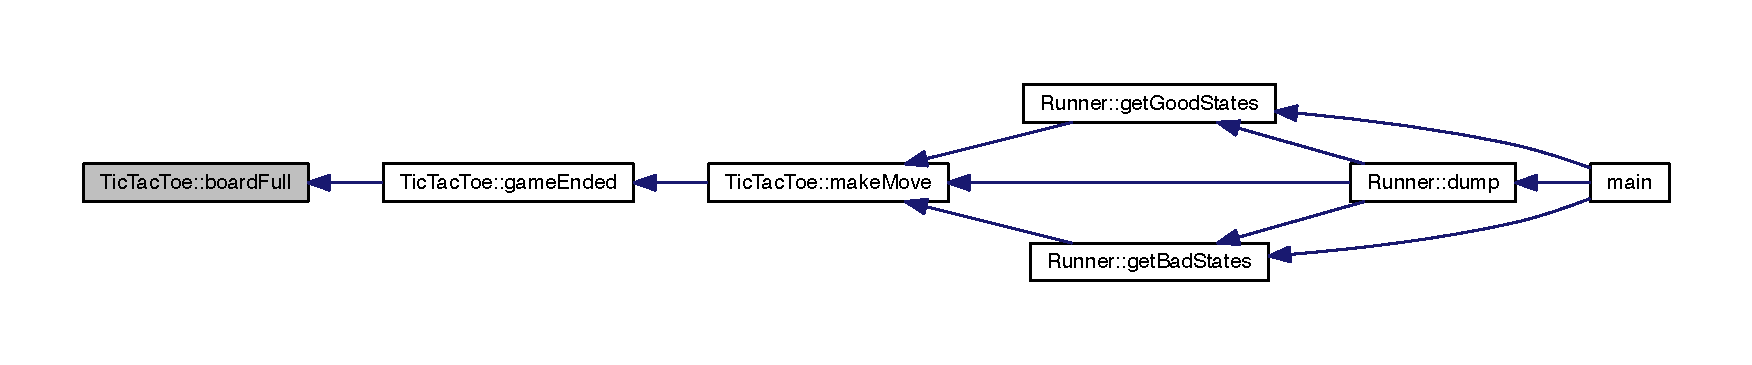
\includegraphics[width=350pt]{class_tic_tac_toe_a750e26d95ced2dca83c21279ef43def9_icgraph}
\end{center}
\end{figure}
\mbox{\Hypertarget{class_tic_tac_toe_a0ed1b3b4b699af8e7db79f502cbc9531}\label{class_tic_tac_toe_a0ed1b3b4b699af8e7db79f502cbc9531}} 
\index{Tic\+Tac\+Toe@{Tic\+Tac\+Toe}!game\+Ended@{game\+Ended}}
\index{game\+Ended@{game\+Ended}!Tic\+Tac\+Toe@{Tic\+Tac\+Toe}}
\subsubsection{\texorpdfstring{game\+Ended()}{gameEnded()}}
{\footnotesize\ttfamily int Tic\+Tac\+Toe\+::game\+Ended (\begin{DoxyParamCaption}{ }\end{DoxyParamCaption})}



Definition at line 36 of file tictactoe.\+cpp.

Here is the call graph for this function\+:\nopagebreak
\begin{figure}[H]
\begin{center}
\leavevmode
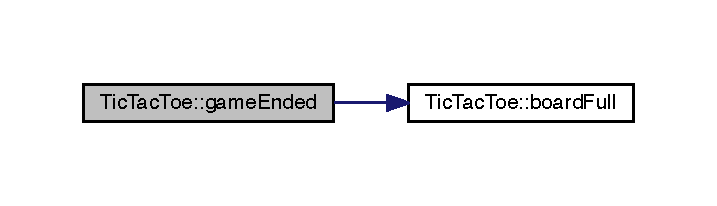
\includegraphics[width=344pt]{class_tic_tac_toe_a0ed1b3b4b699af8e7db79f502cbc9531_cgraph}
\end{center}
\end{figure}
Here is the caller graph for this function\+:\nopagebreak
\begin{figure}[H]
\begin{center}
\leavevmode
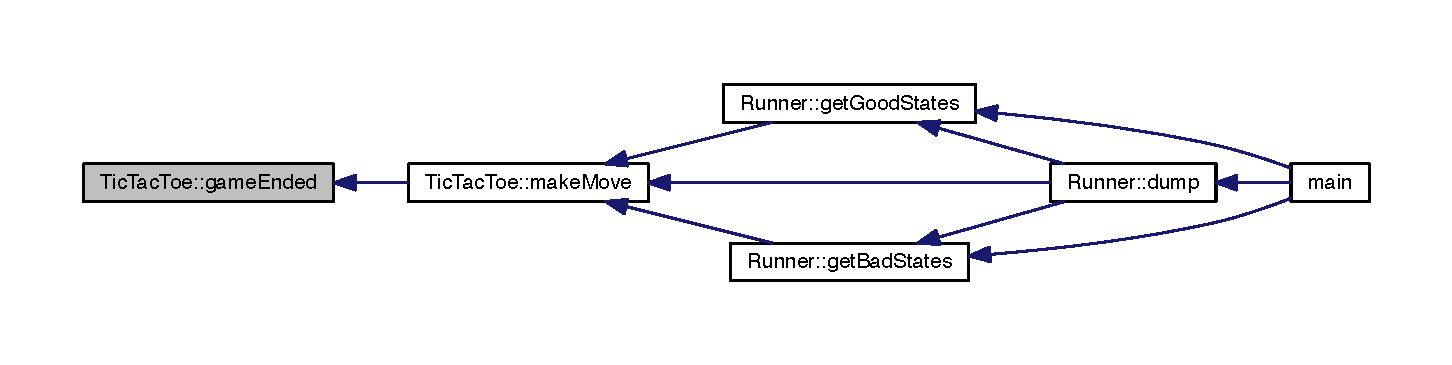
\includegraphics[width=350pt]{class_tic_tac_toe_a0ed1b3b4b699af8e7db79f502cbc9531_icgraph}
\end{center}
\end{figure}
\mbox{\Hypertarget{class_tic_tac_toe_aeacd5865fa7f87f6fd9608b8ed1743a9}\label{class_tic_tac_toe_aeacd5865fa7f87f6fd9608b8ed1743a9}} 
\index{Tic\+Tac\+Toe@{Tic\+Tac\+Toe}!get\+Board@{get\+Board}}
\index{get\+Board@{get\+Board}!Tic\+Tac\+Toe@{Tic\+Tac\+Toe}}
\subsubsection{\texorpdfstring{get\+Board()}{getBoard()}}
{\footnotesize\ttfamily \hyperlink{constants_8h_af901d0acc1572fb0c779f84ddd2c6ce8}{Board} Tic\+Tac\+Toe\+::get\+Board (\begin{DoxyParamCaption}\item[{int}]{player }\end{DoxyParamCaption})}



Definition at line 10 of file tictactoe.\+cpp.

Here is the caller graph for this function\+:\nopagebreak
\begin{figure}[H]
\begin{center}
\leavevmode
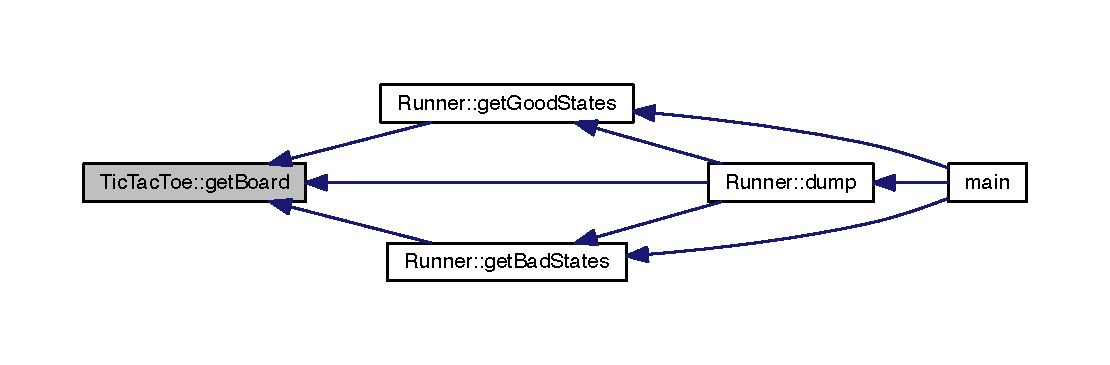
\includegraphics[width=350pt]{class_tic_tac_toe_aeacd5865fa7f87f6fd9608b8ed1743a9_icgraph}
\end{center}
\end{figure}
\mbox{\Hypertarget{class_tic_tac_toe_a597a1911309c9350aa6ce48b817a0e9e}\label{class_tic_tac_toe_a597a1911309c9350aa6ce48b817a0e9e}} 
\index{Tic\+Tac\+Toe@{Tic\+Tac\+Toe}!make\+Move@{make\+Move}}
\index{make\+Move@{make\+Move}!Tic\+Tac\+Toe@{Tic\+Tac\+Toe}}
\subsubsection{\texorpdfstring{make\+Move()}{makeMove()}}
{\footnotesize\ttfamily int Tic\+Tac\+Toe\+::make\+Move (\begin{DoxyParamCaption}\item[{int}]{row,  }\item[{int}]{column,  }\item[{int}]{player }\end{DoxyParamCaption})}



Definition at line 26 of file tictactoe.\+cpp.

Here is the call graph for this function\+:\nopagebreak
\begin{figure}[H]
\begin{center}
\leavevmode
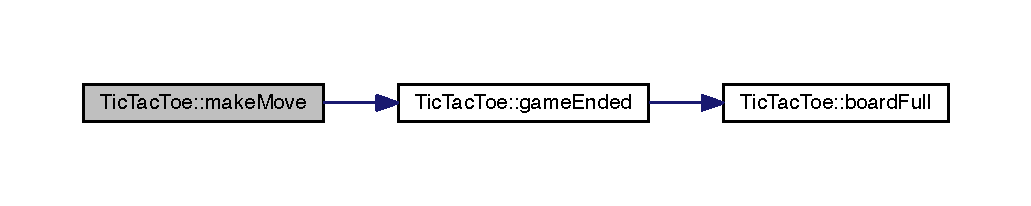
\includegraphics[width=350pt]{class_tic_tac_toe_a597a1911309c9350aa6ce48b817a0e9e_cgraph}
\end{center}
\end{figure}
Here is the caller graph for this function\+:\nopagebreak
\begin{figure}[H]
\begin{center}
\leavevmode
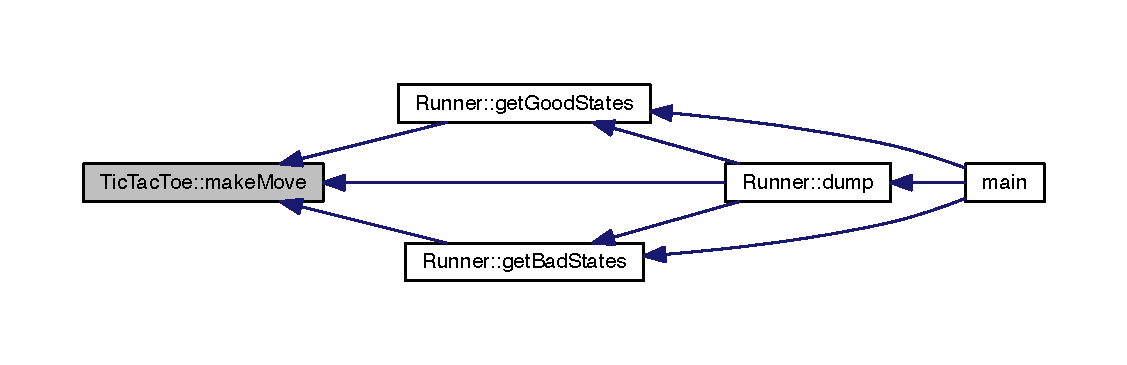
\includegraphics[width=350pt]{class_tic_tac_toe_a597a1911309c9350aa6ce48b817a0e9e_icgraph}
\end{center}
\end{figure}


The documentation for this class was generated from the following files\+:\begin{DoxyCompactItemize}
\item 
\hyperlink{tictactoe_8h}{tictactoe.\+h}\item 
\hyperlink{tictactoe_8cpp}{tictactoe.\+cpp}\end{DoxyCompactItemize}

\chapter{File Documentation}
\hypertarget{ai_8cpp}{}\section{ai.\+cpp File Reference}
\label{ai_8cpp}\index{ai.\+cpp@{ai.\+cpp}}
{\ttfamily \#include \char`\"{}ai.\+h\char`\"{}}\newline
{\ttfamily \#include \char`\"{}neural\+Network.\+h\char`\"{}}\newline
Include dependency graph for ai.\+cpp\+:\nopagebreak
\begin{figure}[H]
\begin{center}
\leavevmode
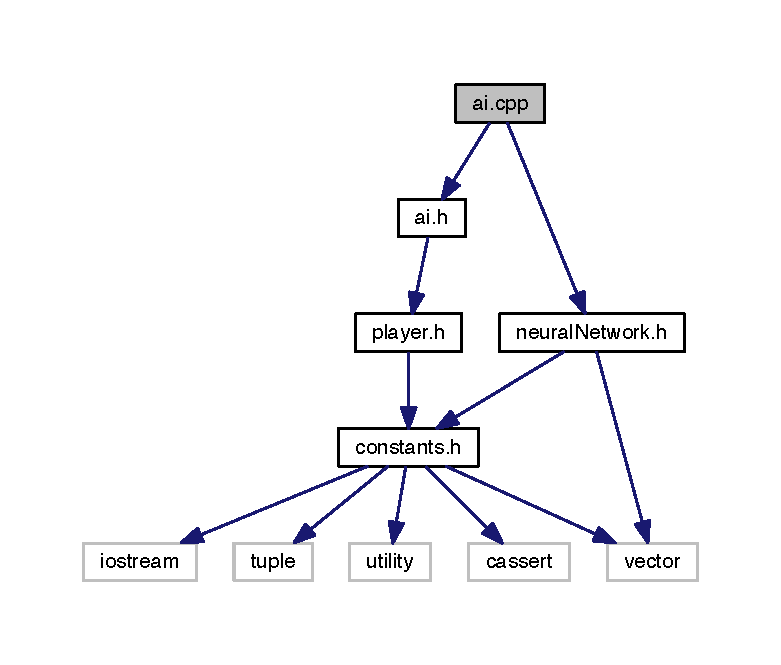
\includegraphics[width=350pt]{ai_8cpp__incl}
\end{center}
\end{figure}

\hypertarget{ai_8h}{}\section{ai.\+h File Reference}
\label{ai_8h}\index{ai.\+h@{ai.\+h}}
{\ttfamily \#include \char`\"{}player.\+h\char`\"{}}\newline
Include dependency graph for ai.\+h\+:\nopagebreak
\begin{figure}[H]
\begin{center}
\leavevmode
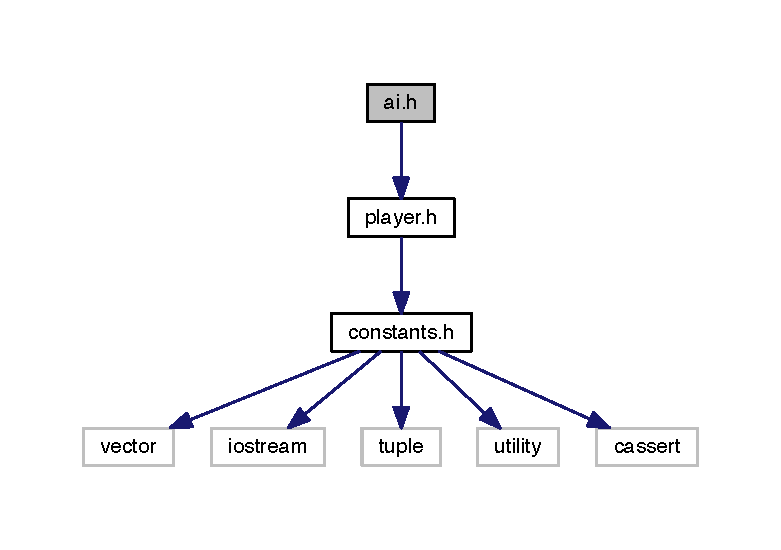
\includegraphics[width=350pt]{ai_8h__incl}
\end{center}
\end{figure}
This graph shows which files directly or indirectly include this file\+:\nopagebreak
\begin{figure}[H]
\begin{center}
\leavevmode
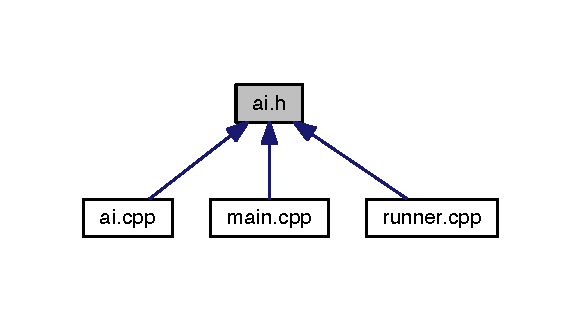
\includegraphics[width=279pt]{ai_8h__dep__incl}
\end{center}
\end{figure}
\subsection*{Classes}
\begin{DoxyCompactItemize}
\item 
class \hyperlink{class_a_i}{AI}
\end{DoxyCompactItemize}
\subsection*{Typedefs}
\begin{DoxyCompactItemize}
\item 
typedef shared\+\_\+ptr$<$ \hyperlink{class_neural_network}{Neural\+Network} $>$ \hyperlink{ai_8h_aafca5132d037883f5cd25160f7ccdc0d}{Neural\+Network\+Ptr}
\end{DoxyCompactItemize}


\subsection{Typedef Documentation}
\mbox{\Hypertarget{ai_8h_aafca5132d037883f5cd25160f7ccdc0d}\label{ai_8h_aafca5132d037883f5cd25160f7ccdc0d}} 
\index{ai.\+h@{ai.\+h}!Neural\+Network\+Ptr@{Neural\+Network\+Ptr}}
\index{Neural\+Network\+Ptr@{Neural\+Network\+Ptr}!ai.\+h@{ai.\+h}}
\subsubsection{\texorpdfstring{Neural\+Network\+Ptr}{NeuralNetworkPtr}}
{\footnotesize\ttfamily typedef shared\+\_\+ptr$<$\hyperlink{class_neural_network}{Neural\+Network}$>$ \hyperlink{ai_8h_aafca5132d037883f5cd25160f7ccdc0d}{Neural\+Network\+Ptr}}



Definition at line 13 of file ai.\+h.


\hypertarget{constants_8cpp}{}\section{constants.\+cpp File Reference}
\label{constants_8cpp}\index{constants.\+cpp@{constants.\+cpp}}
{\ttfamily \#include \char`\"{}constants.\+h\char`\"{}}\newline
{\ttfamily \#include $<$sstream$>$}\newline
Include dependency graph for constants.\+cpp\+:\nopagebreak
\begin{figure}[H]
\begin{center}
\leavevmode
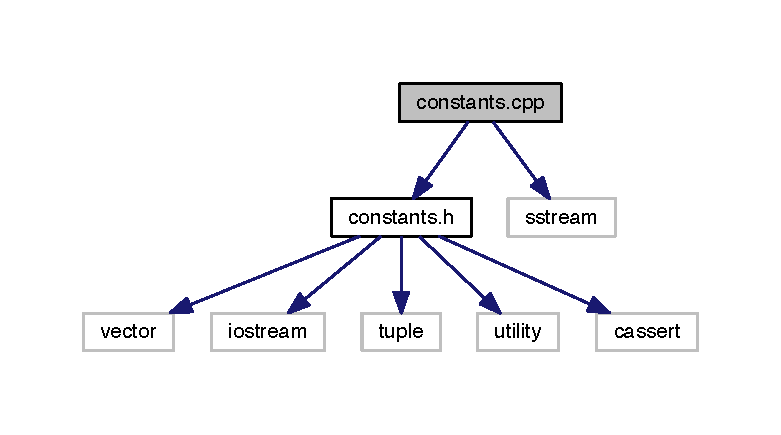
\includegraphics[width=350pt]{constants_8cpp__incl}
\end{center}
\end{figure}
\subsection*{Functions}
\begin{DoxyCompactItemize}
\item 
const char \hyperlink{constants_8cpp_abafaee18c3d094a7c2927d803c996937}{print\+Symbol} (int i)
\item 
void \hyperlink{constants_8cpp_af42f206903df0bc41dfc1d82426bf911}{print\+Move} (\hyperlink{constants_8h_af901d0acc1572fb0c779f84ddd2c6ce8}{Board} \&b, \hyperlink{struct_move}{Move} \&m)
\item 
vector$<$ double $>$ \hyperlink{constants_8cpp_a3bf3485465974fb9c6e137559a43391b}{get\+Node\+Board} (\hyperlink{constants_8h_af901d0acc1572fb0c779f84ddd2c6ce8}{Board} board)
\item 
vector$<$ double $>$ \hyperlink{constants_8cpp_aabbd0f026adcc6f737fe9d2642de970e}{get\+Node\+Move} (\hyperlink{struct_move}{Move} move, bool reverse)
\item 
\hyperlink{struct_move}{Move} \hyperlink{constants_8cpp_a003e3a1a534af97e5d1e75c25ff3be28}{get\+Move\+Node} (vector$<$ double $>$ nodes)
\item 
\hyperlink{struct_move}{Move} \hyperlink{constants_8cpp_a107022faba013a74ef065399a00867af}{get\+Probable\+Move\+From\+Node} (vector$<$ double $>$ nodes)
\item 
vector$<$ double $>$ \& \hyperlink{constants_8cpp_ad17af02b26c5701fec9583eac5a21c3b}{norm} (vector$<$ double $>$ \&v)
\item 
void \hyperlink{constants_8cpp_a0dc3a0d3881d88542de17697bfe32a27}{print\+Board} (\hyperlink{constants_8h_af901d0acc1572fb0c779f84ddd2c6ce8}{Board} \&b)
\item 
void \hyperlink{constants_8cpp_a7fdeaad11fab6949d565928655753fe8}{split} (const std\+::string \&s, char delim, std\+::vector$<$ std\+::string $>$ \&elems)
\item 
double \hyperlink{constants_8cpp_ad29abeca332a1c0701cec6d0204fdc04}{calc\+Error\+Sum} (vector$<$ double $>$ a, vector$<$ double $>$ b)
\item 
ostream \& \hyperlink{constants_8cpp_a500e4d3762c59c6bc5db8783fb6ae952}{operator$<$$<$} (ostream \&os, vector$<$ double $>$ v)
\end{DoxyCompactItemize}


\subsection{Function Documentation}
\mbox{\Hypertarget{constants_8cpp_ad29abeca332a1c0701cec6d0204fdc04}\label{constants_8cpp_ad29abeca332a1c0701cec6d0204fdc04}} 
\index{constants.\+cpp@{constants.\+cpp}!calc\+Error\+Sum@{calc\+Error\+Sum}}
\index{calc\+Error\+Sum@{calc\+Error\+Sum}!constants.\+cpp@{constants.\+cpp}}
\subsubsection{\texorpdfstring{calc\+Error\+Sum()}{calcErrorSum()}}
{\footnotesize\ttfamily double calc\+Error\+Sum (\begin{DoxyParamCaption}\item[{vector$<$ double $>$}]{a,  }\item[{vector$<$ double $>$}]{b }\end{DoxyParamCaption})}



Definition at line 153 of file constants.\+cpp.

Here is the caller graph for this function\+:\nopagebreak
\begin{figure}[H]
\begin{center}
\leavevmode
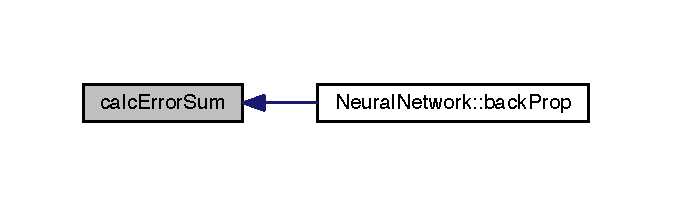
\includegraphics[width=323pt]{constants_8cpp_ad29abeca332a1c0701cec6d0204fdc04_icgraph}
\end{center}
\end{figure}
\mbox{\Hypertarget{constants_8cpp_a003e3a1a534af97e5d1e75c25ff3be28}\label{constants_8cpp_a003e3a1a534af97e5d1e75c25ff3be28}} 
\index{constants.\+cpp@{constants.\+cpp}!get\+Move\+Node@{get\+Move\+Node}}
\index{get\+Move\+Node@{get\+Move\+Node}!constants.\+cpp@{constants.\+cpp}}
\subsubsection{\texorpdfstring{get\+Move\+Node()}{getMoveNode()}}
{\footnotesize\ttfamily \hyperlink{struct_move}{Move} get\+Move\+Node (\begin{DoxyParamCaption}\item[{vector$<$ double $>$}]{nodes }\end{DoxyParamCaption})}



Definition at line 89 of file constants.\+cpp.

Here is the caller graph for this function\+:\nopagebreak
\begin{figure}[H]
\begin{center}
\leavevmode
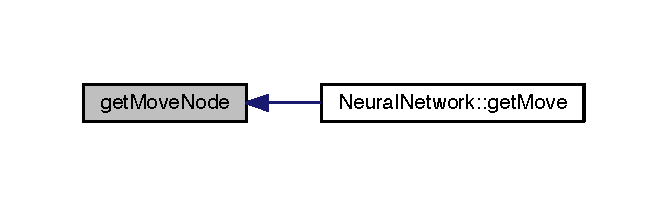
\includegraphics[width=320pt]{constants_8cpp_a003e3a1a534af97e5d1e75c25ff3be28_icgraph}
\end{center}
\end{figure}
\mbox{\Hypertarget{constants_8cpp_a3bf3485465974fb9c6e137559a43391b}\label{constants_8cpp_a3bf3485465974fb9c6e137559a43391b}} 
\index{constants.\+cpp@{constants.\+cpp}!get\+Node\+Board@{get\+Node\+Board}}
\index{get\+Node\+Board@{get\+Node\+Board}!constants.\+cpp@{constants.\+cpp}}
\subsubsection{\texorpdfstring{get\+Node\+Board()}{getNodeBoard()}}
{\footnotesize\ttfamily vector$<$double$>$ get\+Node\+Board (\begin{DoxyParamCaption}\item[{\hyperlink{constants_8h_af901d0acc1572fb0c779f84ddd2c6ce8}{Board}}]{board }\end{DoxyParamCaption})}



Definition at line 54 of file constants.\+cpp.

Here is the caller graph for this function\+:\nopagebreak
\begin{figure}[H]
\begin{center}
\leavevmode
\includegraphics[width=350pt]{constants_8cpp_a3bf3485465974fb9c6e137559a43391b_icgraph}
\end{center}
\end{figure}
\mbox{\Hypertarget{constants_8cpp_aabbd0f026adcc6f737fe9d2642de970e}\label{constants_8cpp_aabbd0f026adcc6f737fe9d2642de970e}} 
\index{constants.\+cpp@{constants.\+cpp}!get\+Node\+Move@{get\+Node\+Move}}
\index{get\+Node\+Move@{get\+Node\+Move}!constants.\+cpp@{constants.\+cpp}}
\subsubsection{\texorpdfstring{get\+Node\+Move()}{getNodeMove()}}
{\footnotesize\ttfamily vector$<$double$>$ get\+Node\+Move (\begin{DoxyParamCaption}\item[{\hyperlink{struct_move}{Move}}]{move,  }\item[{bool}]{reverse }\end{DoxyParamCaption})}



Definition at line 64 of file constants.\+cpp.

Here is the caller graph for this function\+:\nopagebreak
\begin{figure}[H]
\begin{center}
\leavevmode
\includegraphics[width=232pt]{constants_8cpp_aabbd0f026adcc6f737fe9d2642de970e_icgraph}
\end{center}
\end{figure}
\mbox{\Hypertarget{constants_8cpp_a107022faba013a74ef065399a00867af}\label{constants_8cpp_a107022faba013a74ef065399a00867af}} 
\index{constants.\+cpp@{constants.\+cpp}!get\+Probable\+Move\+From\+Node@{get\+Probable\+Move\+From\+Node}}
\index{get\+Probable\+Move\+From\+Node@{get\+Probable\+Move\+From\+Node}!constants.\+cpp@{constants.\+cpp}}
\subsubsection{\texorpdfstring{get\+Probable\+Move\+From\+Node()}{getProbableMoveFromNode()}}
{\footnotesize\ttfamily \hyperlink{struct_move}{Move} get\+Probable\+Move\+From\+Node (\begin{DoxyParamCaption}\item[{vector$<$ double $>$}]{nodes }\end{DoxyParamCaption})}



Definition at line 103 of file constants.\+cpp.

Here is the caller graph for this function\+:\nopagebreak
\begin{figure}[H]
\begin{center}
\leavevmode
\includegraphics[width=350pt]{constants_8cpp_a107022faba013a74ef065399a00867af_icgraph}
\end{center}
\end{figure}
\mbox{\Hypertarget{constants_8cpp_ad17af02b26c5701fec9583eac5a21c3b}\label{constants_8cpp_ad17af02b26c5701fec9583eac5a21c3b}} 
\index{constants.\+cpp@{constants.\+cpp}!norm@{norm}}
\index{norm@{norm}!constants.\+cpp@{constants.\+cpp}}
\subsubsection{\texorpdfstring{norm()}{norm()}}
{\footnotesize\ttfamily vector$<$double$>$\& norm (\begin{DoxyParamCaption}\item[{vector$<$ double $>$ \&}]{v }\end{DoxyParamCaption})}



Definition at line 124 of file constants.\+cpp.

\mbox{\Hypertarget{constants_8cpp_a500e4d3762c59c6bc5db8783fb6ae952}\label{constants_8cpp_a500e4d3762c59c6bc5db8783fb6ae952}} 
\index{constants.\+cpp@{constants.\+cpp}!operator$<$$<$@{operator$<$$<$}}
\index{operator$<$$<$@{operator$<$$<$}!constants.\+cpp@{constants.\+cpp}}
\subsubsection{\texorpdfstring{operator$<$$<$()}{operator<<()}}
{\footnotesize\ttfamily ostream\& operator$<$$<$ (\begin{DoxyParamCaption}\item[{ostream \&}]{os,  }\item[{vector$<$ double $>$}]{v }\end{DoxyParamCaption})}



Definition at line 163 of file constants.\+cpp.

\mbox{\Hypertarget{constants_8cpp_a0dc3a0d3881d88542de17697bfe32a27}\label{constants_8cpp_a0dc3a0d3881d88542de17697bfe32a27}} 
\index{constants.\+cpp@{constants.\+cpp}!print\+Board@{print\+Board}}
\index{print\+Board@{print\+Board}!constants.\+cpp@{constants.\+cpp}}
\subsubsection{\texorpdfstring{print\+Board()}{printBoard()}}
{\footnotesize\ttfamily void print\+Board (\begin{DoxyParamCaption}\item[{\hyperlink{constants_8h_af901d0acc1572fb0c779f84ddd2c6ce8}{Board} \&}]{b }\end{DoxyParamCaption})}



Definition at line 133 of file constants.\+cpp.

Here is the call graph for this function\+:\nopagebreak
\begin{figure}[H]
\begin{center}
\leavevmode
\includegraphics[width=247pt]{constants_8cpp_a0dc3a0d3881d88542de17697bfe32a27_cgraph}
\end{center}
\end{figure}
Here is the caller graph for this function\+:\nopagebreak
\begin{figure}[H]
\begin{center}
\leavevmode
\includegraphics[width=270pt]{constants_8cpp_a0dc3a0d3881d88542de17697bfe32a27_icgraph}
\end{center}
\end{figure}
\mbox{\Hypertarget{constants_8cpp_af42f206903df0bc41dfc1d82426bf911}\label{constants_8cpp_af42f206903df0bc41dfc1d82426bf911}} 
\index{constants.\+cpp@{constants.\+cpp}!print\+Move@{print\+Move}}
\index{print\+Move@{print\+Move}!constants.\+cpp@{constants.\+cpp}}
\subsubsection{\texorpdfstring{print\+Move()}{printMove()}}
{\footnotesize\ttfamily void print\+Move (\begin{DoxyParamCaption}\item[{\hyperlink{constants_8h_af901d0acc1572fb0c779f84ddd2c6ce8}{Board} \&}]{b,  }\item[{\hyperlink{struct_move}{Move} \&}]{m }\end{DoxyParamCaption})}



Definition at line 30 of file constants.\+cpp.

Here is the call graph for this function\+:\nopagebreak
\begin{figure}[H]
\begin{center}
\leavevmode
\includegraphics[width=245pt]{constants_8cpp_af42f206903df0bc41dfc1d82426bf911_cgraph}
\end{center}
\end{figure}
Here is the caller graph for this function\+:\nopagebreak
\begin{figure}[H]
\begin{center}
\leavevmode
\includegraphics[width=329pt]{constants_8cpp_af42f206903df0bc41dfc1d82426bf911_icgraph}
\end{center}
\end{figure}
\mbox{\Hypertarget{constants_8cpp_abafaee18c3d094a7c2927d803c996937}\label{constants_8cpp_abafaee18c3d094a7c2927d803c996937}} 
\index{constants.\+cpp@{constants.\+cpp}!print\+Symbol@{print\+Symbol}}
\index{print\+Symbol@{print\+Symbol}!constants.\+cpp@{constants.\+cpp}}
\subsubsection{\texorpdfstring{print\+Symbol()}{printSymbol()}}
{\footnotesize\ttfamily const char print\+Symbol (\begin{DoxyParamCaption}\item[{int}]{i }\end{DoxyParamCaption})}



Definition at line 17 of file constants.\+cpp.

Here is the caller graph for this function\+:\nopagebreak
\begin{figure}[H]
\begin{center}
\leavevmode
\includegraphics[width=350pt]{constants_8cpp_abafaee18c3d094a7c2927d803c996937_icgraph}
\end{center}
\end{figure}
\mbox{\Hypertarget{constants_8cpp_a7fdeaad11fab6949d565928655753fe8}\label{constants_8cpp_a7fdeaad11fab6949d565928655753fe8}} 
\index{constants.\+cpp@{constants.\+cpp}!split@{split}}
\index{split@{split}!constants.\+cpp@{constants.\+cpp}}
\subsubsection{\texorpdfstring{split()}{split()}}
{\footnotesize\ttfamily void split (\begin{DoxyParamCaption}\item[{const std\+::string \&}]{s,  }\item[{char}]{delim,  }\item[{std\+::vector$<$ std\+::string $>$ \&}]{elems }\end{DoxyParamCaption})}



Definition at line 144 of file constants.\+cpp.

Here is the caller graph for this function\+:\nopagebreak
\begin{figure}[H]
\begin{center}
\leavevmode
\includegraphics[width=304pt]{constants_8cpp_a7fdeaad11fab6949d565928655753fe8_icgraph}
\end{center}
\end{figure}

\hypertarget{constants_8h}{}\section{constants.\+h File Reference}
\label{constants_8h}\index{constants.\+h@{constants.\+h}}
{\ttfamily \#include $<$vector$>$}\newline
{\ttfamily \#include $<$iostream$>$}\newline
{\ttfamily \#include $<$tuple$>$}\newline
{\ttfamily \#include $<$utility$>$}\newline
{\ttfamily \#include $<$cassert$>$}\newline
Include dependency graph for constants.\+h\+:\nopagebreak
\begin{figure}[H]
\begin{center}
\leavevmode
\includegraphics[width=350pt]{constants_8h__incl}
\end{center}
\end{figure}
This graph shows which files directly or indirectly include this file\+:\nopagebreak
\begin{figure}[H]
\begin{center}
\leavevmode
\includegraphics[width=350pt]{constants_8h__dep__incl}
\end{center}
\end{figure}
\subsection*{Classes}
\begin{DoxyCompactItemize}
\item 
struct \hyperlink{struct_move}{Move}
\end{DoxyCompactItemize}
\subsection*{Macros}
\begin{DoxyCompactItemize}
\item 
\#define \hyperlink{constants_8h_ad72dbcf6d0153db1b8d8a58001feed83}{D\+E\+B\+UG}
\end{DoxyCompactItemize}
\subsection*{Typedefs}
\begin{DoxyCompactItemize}
\item 
typedef vector$<$ vector$<$ int $>$ $>$ \hyperlink{constants_8h_af901d0acc1572fb0c779f84ddd2c6ce8}{Board}
\item 
typedef std\+::pair$<$ \hyperlink{constants_8h_af901d0acc1572fb0c779f84ddd2c6ce8}{Board}, \hyperlink{struct_move}{Move} $>$ \hyperlink{constants_8h_afd2599a4148deb913a46b4e2eba9e68a}{State}
\end{DoxyCompactItemize}
\subsection*{Functions}
\begin{DoxyCompactItemize}
\item 
{\footnotesize template$<$typename T $>$ }\\int \hyperlink{constants_8h_a1ab31b90bc584c635ec159468ceed9b2}{sgn} (T val)
\item 
const char \hyperlink{constants_8h_abafaee18c3d094a7c2927d803c996937}{print\+Symbol} (int i)
\item 
void \hyperlink{constants_8h_af42f206903df0bc41dfc1d82426bf911}{print\+Move} (\hyperlink{constants_8h_af901d0acc1572fb0c779f84ddd2c6ce8}{Board} \&b, \hyperlink{struct_move}{Move} \&m)
\item 
vector$<$ double $>$ \hyperlink{constants_8h_a3bf3485465974fb9c6e137559a43391b}{get\+Node\+Board} (\hyperlink{constants_8h_af901d0acc1572fb0c779f84ddd2c6ce8}{Board} board)
\item 
vector$<$ double $>$ \hyperlink{constants_8h_ac725637b6a5e5db50481c7a2102a1b7b}{get\+Node\+Move} (\hyperlink{struct_move}{Move} move, bool reverse=false)
\item 
\hyperlink{constants_8h_af901d0acc1572fb0c779f84ddd2c6ce8}{Board} \hyperlink{constants_8h_ac40651b5fe736205ebd6bb6e1e8cdc94}{get\+Board\+Node} (vector$<$ double $>$ nodes)
\item 
\hyperlink{struct_move}{Move} \hyperlink{constants_8h_a003e3a1a534af97e5d1e75c25ff3be28}{get\+Move\+Node} (vector$<$ double $>$ nodes)
\item 
\hyperlink{struct_move}{Move} \hyperlink{constants_8h_a107022faba013a74ef065399a00867af}{get\+Probable\+Move\+From\+Node} (vector$<$ double $>$ nodes)
\item 
vector$<$ double $>$ \& \hyperlink{constants_8h_ad17af02b26c5701fec9583eac5a21c3b}{norm} (vector$<$ double $>$ \&v)
\item 
void \hyperlink{constants_8h_a0dc3a0d3881d88542de17697bfe32a27}{print\+Board} (\hyperlink{constants_8h_af901d0acc1572fb0c779f84ddd2c6ce8}{Board} \&b)
\item 
void \hyperlink{constants_8h_a7fdeaad11fab6949d565928655753fe8}{split} (const std\+::string \&s, char delim, std\+::vector$<$ std\+::string $>$ \&elems)
\item 
double \hyperlink{constants_8h_ad29abeca332a1c0701cec6d0204fdc04}{calc\+Error\+Sum} (vector$<$ double $>$ a, vector$<$ double $>$ b)
\item 
ostream \& \hyperlink{constants_8h_a500e4d3762c59c6bc5db8783fb6ae952}{operator$<$$<$} (ostream \&os, vector$<$ double $>$ v)
\end{DoxyCompactItemize}
\subsection*{Variables}
\begin{DoxyCompactItemize}
\item 
const int \hyperlink{constants_8h_aa8b29b5b761ea6c3211d1280a7bf8c19}{cross} = 1
\item 
const int \hyperlink{constants_8h_a27dc2586694a3ec69f34b6979008aec2}{circle} = 2
\item 
const unsigned \hyperlink{constants_8h_a93235db48216bba8e4618b0ec77b5d6a}{D\+E\+C\+I\+M\+A\+LS} = 4
\item 
const vector$<$ vector$<$ vector$<$ int $>$ $>$ $>$ \hyperlink{constants_8h_a902cdcde74b519151ed624b0e9aad266}{winning\+Positions}
\item 
const \hyperlink{constants_8h_af901d0acc1572fb0c779f84ddd2c6ce8}{Board} \hyperlink{constants_8h_af5fb8bae1f8e7bdfd9b2ad677d668a27}{empyt\+Board} = \{ \{ 0, 0, 0 \}, \{ 0, 0, 0 \}, \{ 0, 0, 0 \} \}
\end{DoxyCompactItemize}


\subsection{Macro Definition Documentation}
\mbox{\Hypertarget{constants_8h_ad72dbcf6d0153db1b8d8a58001feed83}\label{constants_8h_ad72dbcf6d0153db1b8d8a58001feed83}} 
\index{constants.\+h@{constants.\+h}!D\+E\+B\+UG@{D\+E\+B\+UG}}
\index{D\+E\+B\+UG@{D\+E\+B\+UG}!constants.\+h@{constants.\+h}}
\subsubsection{\texorpdfstring{D\+E\+B\+UG}{DEBUG}}
{\footnotesize\ttfamily \#define D\+E\+B\+UG}



Definition at line 9 of file constants.\+h.



\subsection{Typedef Documentation}
\mbox{\Hypertarget{constants_8h_af901d0acc1572fb0c779f84ddd2c6ce8}\label{constants_8h_af901d0acc1572fb0c779f84ddd2c6ce8}} 
\index{constants.\+h@{constants.\+h}!Board@{Board}}
\index{Board@{Board}!constants.\+h@{constants.\+h}}
\subsubsection{\texorpdfstring{Board}{Board}}
{\footnotesize\ttfamily typedef vector$<$vector$<$int$>$ $>$ \hyperlink{constants_8h_af901d0acc1572fb0c779f84ddd2c6ce8}{Board}}



Definition at line 19 of file constants.\+h.

\mbox{\Hypertarget{constants_8h_afd2599a4148deb913a46b4e2eba9e68a}\label{constants_8h_afd2599a4148deb913a46b4e2eba9e68a}} 
\index{constants.\+h@{constants.\+h}!State@{State}}
\index{State@{State}!constants.\+h@{constants.\+h}}
\subsubsection{\texorpdfstring{State}{State}}
{\footnotesize\ttfamily typedef std\+::pair$<$\hyperlink{constants_8h_af901d0acc1572fb0c779f84ddd2c6ce8}{Board}, \hyperlink{struct_move}{Move}$>$ \hyperlink{constants_8h_afd2599a4148deb913a46b4e2eba9e68a}{State}}



Definition at line 20 of file constants.\+h.



\subsection{Function Documentation}
\mbox{\Hypertarget{constants_8h_ad29abeca332a1c0701cec6d0204fdc04}\label{constants_8h_ad29abeca332a1c0701cec6d0204fdc04}} 
\index{constants.\+h@{constants.\+h}!calc\+Error\+Sum@{calc\+Error\+Sum}}
\index{calc\+Error\+Sum@{calc\+Error\+Sum}!constants.\+h@{constants.\+h}}
\subsubsection{\texorpdfstring{calc\+Error\+Sum()}{calcErrorSum()}}
{\footnotesize\ttfamily double calc\+Error\+Sum (\begin{DoxyParamCaption}\item[{vector$<$ double $>$}]{a,  }\item[{vector$<$ double $>$}]{b }\end{DoxyParamCaption})}



Definition at line 153 of file constants.\+cpp.

Here is the caller graph for this function\+:\nopagebreak
\begin{figure}[H]
\begin{center}
\leavevmode
\includegraphics[width=323pt]{constants_8h_ad29abeca332a1c0701cec6d0204fdc04_icgraph}
\end{center}
\end{figure}
\mbox{\Hypertarget{constants_8h_ac40651b5fe736205ebd6bb6e1e8cdc94}\label{constants_8h_ac40651b5fe736205ebd6bb6e1e8cdc94}} 
\index{constants.\+h@{constants.\+h}!get\+Board\+Node@{get\+Board\+Node}}
\index{get\+Board\+Node@{get\+Board\+Node}!constants.\+h@{constants.\+h}}
\subsubsection{\texorpdfstring{get\+Board\+Node()}{getBoardNode()}}
{\footnotesize\ttfamily \hyperlink{constants_8h_af901d0acc1572fb0c779f84ddd2c6ce8}{Board} get\+Board\+Node (\begin{DoxyParamCaption}\item[{vector$<$ double $>$}]{nodes }\end{DoxyParamCaption})}

\mbox{\Hypertarget{constants_8h_a003e3a1a534af97e5d1e75c25ff3be28}\label{constants_8h_a003e3a1a534af97e5d1e75c25ff3be28}} 
\index{constants.\+h@{constants.\+h}!get\+Move\+Node@{get\+Move\+Node}}
\index{get\+Move\+Node@{get\+Move\+Node}!constants.\+h@{constants.\+h}}
\subsubsection{\texorpdfstring{get\+Move\+Node()}{getMoveNode()}}
{\footnotesize\ttfamily \hyperlink{struct_move}{Move} get\+Move\+Node (\begin{DoxyParamCaption}\item[{vector$<$ double $>$}]{nodes }\end{DoxyParamCaption})}



Definition at line 89 of file constants.\+cpp.

Here is the caller graph for this function\+:\nopagebreak
\begin{figure}[H]
\begin{center}
\leavevmode
\includegraphics[width=320pt]{constants_8h_a003e3a1a534af97e5d1e75c25ff3be28_icgraph}
\end{center}
\end{figure}
\mbox{\Hypertarget{constants_8h_a3bf3485465974fb9c6e137559a43391b}\label{constants_8h_a3bf3485465974fb9c6e137559a43391b}} 
\index{constants.\+h@{constants.\+h}!get\+Node\+Board@{get\+Node\+Board}}
\index{get\+Node\+Board@{get\+Node\+Board}!constants.\+h@{constants.\+h}}
\subsubsection{\texorpdfstring{get\+Node\+Board()}{getNodeBoard()}}
{\footnotesize\ttfamily vector$<$double$>$ get\+Node\+Board (\begin{DoxyParamCaption}\item[{\hyperlink{constants_8h_af901d0acc1572fb0c779f84ddd2c6ce8}{Board}}]{board }\end{DoxyParamCaption})}



Definition at line 54 of file constants.\+cpp.

Here is the caller graph for this function\+:\nopagebreak
\begin{figure}[H]
\begin{center}
\leavevmode
\includegraphics[width=350pt]{constants_8h_a3bf3485465974fb9c6e137559a43391b_icgraph}
\end{center}
\end{figure}
\mbox{\Hypertarget{constants_8h_ac725637b6a5e5db50481c7a2102a1b7b}\label{constants_8h_ac725637b6a5e5db50481c7a2102a1b7b}} 
\index{constants.\+h@{constants.\+h}!get\+Node\+Move@{get\+Node\+Move}}
\index{get\+Node\+Move@{get\+Node\+Move}!constants.\+h@{constants.\+h}}
\subsubsection{\texorpdfstring{get\+Node\+Move()}{getNodeMove()}}
{\footnotesize\ttfamily vector$<$double$>$ get\+Node\+Move (\begin{DoxyParamCaption}\item[{\hyperlink{struct_move}{Move}}]{move,  }\item[{bool}]{reverse = {\ttfamily false} }\end{DoxyParamCaption})}



Definition at line 64 of file constants.\+cpp.

Here is the caller graph for this function\+:\nopagebreak
\begin{figure}[H]
\begin{center}
\leavevmode
\includegraphics[width=232pt]{constants_8h_ac725637b6a5e5db50481c7a2102a1b7b_icgraph}
\end{center}
\end{figure}
\mbox{\Hypertarget{constants_8h_a107022faba013a74ef065399a00867af}\label{constants_8h_a107022faba013a74ef065399a00867af}} 
\index{constants.\+h@{constants.\+h}!get\+Probable\+Move\+From\+Node@{get\+Probable\+Move\+From\+Node}}
\index{get\+Probable\+Move\+From\+Node@{get\+Probable\+Move\+From\+Node}!constants.\+h@{constants.\+h}}
\subsubsection{\texorpdfstring{get\+Probable\+Move\+From\+Node()}{getProbableMoveFromNode()}}
{\footnotesize\ttfamily \hyperlink{struct_move}{Move} get\+Probable\+Move\+From\+Node (\begin{DoxyParamCaption}\item[{vector$<$ double $>$}]{nodes }\end{DoxyParamCaption})}



Definition at line 103 of file constants.\+cpp.

Here is the caller graph for this function\+:\nopagebreak
\begin{figure}[H]
\begin{center}
\leavevmode
\includegraphics[width=350pt]{constants_8h_a107022faba013a74ef065399a00867af_icgraph}
\end{center}
\end{figure}
\mbox{\Hypertarget{constants_8h_ad17af02b26c5701fec9583eac5a21c3b}\label{constants_8h_ad17af02b26c5701fec9583eac5a21c3b}} 
\index{constants.\+h@{constants.\+h}!norm@{norm}}
\index{norm@{norm}!constants.\+h@{constants.\+h}}
\subsubsection{\texorpdfstring{norm()}{norm()}}
{\footnotesize\ttfamily vector$<$double$>$\& norm (\begin{DoxyParamCaption}\item[{vector$<$ double $>$ \&}]{v }\end{DoxyParamCaption})}



Definition at line 124 of file constants.\+cpp.

\mbox{\Hypertarget{constants_8h_a500e4d3762c59c6bc5db8783fb6ae952}\label{constants_8h_a500e4d3762c59c6bc5db8783fb6ae952}} 
\index{constants.\+h@{constants.\+h}!operator$<$$<$@{operator$<$$<$}}
\index{operator$<$$<$@{operator$<$$<$}!constants.\+h@{constants.\+h}}
\subsubsection{\texorpdfstring{operator$<$$<$()}{operator<<()}}
{\footnotesize\ttfamily ostream\& operator$<$$<$ (\begin{DoxyParamCaption}\item[{ostream \&}]{os,  }\item[{vector$<$ double $>$}]{v }\end{DoxyParamCaption})}



Definition at line 163 of file constants.\+cpp.

\mbox{\Hypertarget{constants_8h_a0dc3a0d3881d88542de17697bfe32a27}\label{constants_8h_a0dc3a0d3881d88542de17697bfe32a27}} 
\index{constants.\+h@{constants.\+h}!print\+Board@{print\+Board}}
\index{print\+Board@{print\+Board}!constants.\+h@{constants.\+h}}
\subsubsection{\texorpdfstring{print\+Board()}{printBoard()}}
{\footnotesize\ttfamily void print\+Board (\begin{DoxyParamCaption}\item[{\hyperlink{constants_8h_af901d0acc1572fb0c779f84ddd2c6ce8}{Board} \&}]{b }\end{DoxyParamCaption})}



Definition at line 133 of file constants.\+cpp.

Here is the call graph for this function\+:\nopagebreak
\begin{figure}[H]
\begin{center}
\leavevmode
\includegraphics[width=247pt]{constants_8h_a0dc3a0d3881d88542de17697bfe32a27_cgraph}
\end{center}
\end{figure}
Here is the caller graph for this function\+:\nopagebreak
\begin{figure}[H]
\begin{center}
\leavevmode
\includegraphics[width=270pt]{constants_8h_a0dc3a0d3881d88542de17697bfe32a27_icgraph}
\end{center}
\end{figure}
\mbox{\Hypertarget{constants_8h_af42f206903df0bc41dfc1d82426bf911}\label{constants_8h_af42f206903df0bc41dfc1d82426bf911}} 
\index{constants.\+h@{constants.\+h}!print\+Move@{print\+Move}}
\index{print\+Move@{print\+Move}!constants.\+h@{constants.\+h}}
\subsubsection{\texorpdfstring{print\+Move()}{printMove()}}
{\footnotesize\ttfamily void print\+Move (\begin{DoxyParamCaption}\item[{\hyperlink{constants_8h_af901d0acc1572fb0c779f84ddd2c6ce8}{Board} \&}]{b,  }\item[{\hyperlink{struct_move}{Move} \&}]{m }\end{DoxyParamCaption})}



Definition at line 30 of file constants.\+cpp.

Here is the call graph for this function\+:\nopagebreak
\begin{figure}[H]
\begin{center}
\leavevmode
\includegraphics[width=245pt]{constants_8h_af42f206903df0bc41dfc1d82426bf911_cgraph}
\end{center}
\end{figure}
Here is the caller graph for this function\+:\nopagebreak
\begin{figure}[H]
\begin{center}
\leavevmode
\includegraphics[width=329pt]{constants_8h_af42f206903df0bc41dfc1d82426bf911_icgraph}
\end{center}
\end{figure}
\mbox{\Hypertarget{constants_8h_abafaee18c3d094a7c2927d803c996937}\label{constants_8h_abafaee18c3d094a7c2927d803c996937}} 
\index{constants.\+h@{constants.\+h}!print\+Symbol@{print\+Symbol}}
\index{print\+Symbol@{print\+Symbol}!constants.\+h@{constants.\+h}}
\subsubsection{\texorpdfstring{print\+Symbol()}{printSymbol()}}
{\footnotesize\ttfamily const char print\+Symbol (\begin{DoxyParamCaption}\item[{int}]{i }\end{DoxyParamCaption})}



Definition at line 17 of file constants.\+cpp.

Here is the caller graph for this function\+:\nopagebreak
\begin{figure}[H]
\begin{center}
\leavevmode
\includegraphics[width=350pt]{constants_8h_abafaee18c3d094a7c2927d803c996937_icgraph}
\end{center}
\end{figure}
\mbox{\Hypertarget{constants_8h_a1ab31b90bc584c635ec159468ceed9b2}\label{constants_8h_a1ab31b90bc584c635ec159468ceed9b2}} 
\index{constants.\+h@{constants.\+h}!sgn@{sgn}}
\index{sgn@{sgn}!constants.\+h@{constants.\+h}}
\subsubsection{\texorpdfstring{sgn()}{sgn()}}
{\footnotesize\ttfamily template$<$typename T $>$ \\
int sgn (\begin{DoxyParamCaption}\item[{T}]{val }\end{DoxyParamCaption})}



Definition at line 41 of file constants.\+h.

\mbox{\Hypertarget{constants_8h_a7fdeaad11fab6949d565928655753fe8}\label{constants_8h_a7fdeaad11fab6949d565928655753fe8}} 
\index{constants.\+h@{constants.\+h}!split@{split}}
\index{split@{split}!constants.\+h@{constants.\+h}}
\subsubsection{\texorpdfstring{split()}{split()}}
{\footnotesize\ttfamily void split (\begin{DoxyParamCaption}\item[{const std\+::string \&}]{s,  }\item[{char}]{delim,  }\item[{std\+::vector$<$ std\+::string $>$ \&}]{elems }\end{DoxyParamCaption})}



Definition at line 144 of file constants.\+cpp.

Here is the caller graph for this function\+:\nopagebreak
\begin{figure}[H]
\begin{center}
\leavevmode
\includegraphics[width=304pt]{constants_8h_a7fdeaad11fab6949d565928655753fe8_icgraph}
\end{center}
\end{figure}


\subsection{Variable Documentation}
\mbox{\Hypertarget{constants_8h_a27dc2586694a3ec69f34b6979008aec2}\label{constants_8h_a27dc2586694a3ec69f34b6979008aec2}} 
\index{constants.\+h@{constants.\+h}!circle@{circle}}
\index{circle@{circle}!constants.\+h@{constants.\+h}}
\subsubsection{\texorpdfstring{circle}{circle}}
{\footnotesize\ttfamily const int circle = 2}



Definition at line 22 of file constants.\+h.

\mbox{\Hypertarget{constants_8h_aa8b29b5b761ea6c3211d1280a7bf8c19}\label{constants_8h_aa8b29b5b761ea6c3211d1280a7bf8c19}} 
\index{constants.\+h@{constants.\+h}!cross@{cross}}
\index{cross@{cross}!constants.\+h@{constants.\+h}}
\subsubsection{\texorpdfstring{cross}{cross}}
{\footnotesize\ttfamily const int cross = 1}



Definition at line 21 of file constants.\+h.

\mbox{\Hypertarget{constants_8h_a93235db48216bba8e4618b0ec77b5d6a}\label{constants_8h_a93235db48216bba8e4618b0ec77b5d6a}} 
\index{constants.\+h@{constants.\+h}!D\+E\+C\+I\+M\+A\+LS@{D\+E\+C\+I\+M\+A\+LS}}
\index{D\+E\+C\+I\+M\+A\+LS@{D\+E\+C\+I\+M\+A\+LS}!constants.\+h@{constants.\+h}}
\subsubsection{\texorpdfstring{D\+E\+C\+I\+M\+A\+LS}{DECIMALS}}
{\footnotesize\ttfamily const unsigned D\+E\+C\+I\+M\+A\+LS = 4}



Definition at line 24 of file constants.\+h.

\mbox{\Hypertarget{constants_8h_af5fb8bae1f8e7bdfd9b2ad677d668a27}\label{constants_8h_af5fb8bae1f8e7bdfd9b2ad677d668a27}} 
\index{constants.\+h@{constants.\+h}!empyt\+Board@{empyt\+Board}}
\index{empyt\+Board@{empyt\+Board}!constants.\+h@{constants.\+h}}
\subsubsection{\texorpdfstring{empyt\+Board}{empytBoard}}
{\footnotesize\ttfamily const \hyperlink{constants_8h_af901d0acc1572fb0c779f84ddd2c6ce8}{Board} empyt\+Board = \{ \{ 0, 0, 0 \}, \{ 0, 0, 0 \}, \{ 0, 0, 0 \} \}}



Definition at line 51 of file constants.\+h.

\mbox{\Hypertarget{constants_8h_a902cdcde74b519151ed624b0e9aad266}\label{constants_8h_a902cdcde74b519151ed624b0e9aad266}} 
\index{constants.\+h@{constants.\+h}!winning\+Positions@{winning\+Positions}}
\index{winning\+Positions@{winning\+Positions}!constants.\+h@{constants.\+h}}
\subsubsection{\texorpdfstring{winning\+Positions}{winningPositions}}
{\footnotesize\ttfamily const vector$<$vector$<$vector$<$int$>$ $>$ $>$ winning\+Positions}

{\bfseries Initial value\+:}
\begin{DoxyCode}
= \{ \{ \{ 0, 0 \}, \{ 1, 0 \}, \{
        2, 0 \} \}, \{ \{ 0, 1 \}, \{ 1, 1 \}, \{ 2, 1 \} \}, \{ \{ 0, 2 \}, \{ 1, 2 \},
        \{ 2, 2 \} \}, \{ \{ 0, 0 \}, \{ 0, 1 \}, \{ 0, 2 \} \}, \{ \{ 1, 0 \}, \{ 1, 1 \}, \{ 1,
        2 \} \}, \{ \{ 2, 0 \}, \{ 2, 1 \}, \{ 2, 2 \} \},
        \{ \{ 0, 0 \}, \{ 1, 1 \}, \{ 2, 2 \} \}, \{ \{ 0, 2 \}, \{ 1, 1 \}, \{ 2, 0 \} \}, \}
\end{DoxyCode}


Definition at line 45 of file constants.\+h.


\hypertarget{human_8cpp}{}\section{human.\+cpp File Reference}
\label{human_8cpp}\index{human.\+cpp@{human.\+cpp}}
{\ttfamily \#include \char`\"{}human.\+h\char`\"{}}\newline
Include dependency graph for human.\+cpp\+:\nopagebreak
\begin{figure}[H]
\begin{center}
\leavevmode
\includegraphics[width=350pt]{human_8cpp__incl}
\end{center}
\end{figure}

\hypertarget{human_8h}{}\section{human.\+h File Reference}
\label{human_8h}\index{human.\+h@{human.\+h}}
{\ttfamily \#include \char`\"{}player.\+h\char`\"{}}\newline
Include dependency graph for human.\+h\+:\nopagebreak
\begin{figure}[H]
\begin{center}
\leavevmode
\includegraphics[width=350pt]{human_8h__incl}
\end{center}
\end{figure}
This graph shows which files directly or indirectly include this file\+:\nopagebreak
\begin{figure}[H]
\begin{center}
\leavevmode
\includegraphics[width=301pt]{human_8h__dep__incl}
\end{center}
\end{figure}
\subsection*{Classes}
\begin{DoxyCompactItemize}
\item 
class \hyperlink{class_human}{Human}
\end{DoxyCompactItemize}

\hypertarget{loading_bar_8cpp}{}\section{loading\+Bar.\+cpp File Reference}
\label{loading_bar_8cpp}\index{loading\+Bar.\+cpp@{loading\+Bar.\+cpp}}
{\ttfamily \#include \char`\"{}loading\+Bar.\+h\char`\"{}}\newline
{\ttfamily \#include $<$cmath$>$}\newline
{\ttfamily \#include $<$ctime$>$}\newline
{\ttfamily \#include $<$chrono$>$}\newline
{\ttfamily \#include $<$iostream$>$}\newline
Include dependency graph for loading\+Bar.\+cpp\+:\nopagebreak
\begin{figure}[H]
\begin{center}
\leavevmode
\includegraphics[width=350pt]{loading_bar_8cpp__incl}
\end{center}
\end{figure}

\hypertarget{loading_bar_8h}{}\section{loading\+Bar.\+h File Reference}
\label{loading_bar_8h}\index{loading\+Bar.\+h@{loading\+Bar.\+h}}
{\ttfamily \#include $<$chrono$>$}\newline
{\ttfamily \#include $<$string$>$}\newline
Include dependency graph for loading\+Bar.\+h\+:\nopagebreak
\begin{figure}[H]
\begin{center}
\leavevmode
\includegraphics[width=186pt]{loading_bar_8h__incl}
\end{center}
\end{figure}
This graph shows which files directly or indirectly include this file\+:\nopagebreak
\begin{figure}[H]
\begin{center}
\leavevmode
\includegraphics[width=236pt]{loading_bar_8h__dep__incl}
\end{center}
\end{figure}
\subsection*{Classes}
\begin{DoxyCompactItemize}
\item 
class \hyperlink{class_loading_bar}{Loading\+Bar}
\end{DoxyCompactItemize}

\hypertarget{logic_player_8cpp}{}\section{logic\+Player.\+cpp File Reference}
\label{logic_player_8cpp}\index{logic\+Player.\+cpp@{logic\+Player.\+cpp}}
{\ttfamily \#include \char`\"{}logic\+Player.\+h\char`\"{}}\newline
Include dependency graph for logic\+Player.\+cpp\+:\nopagebreak
\begin{figure}[H]
\begin{center}
\leavevmode
\includegraphics[width=350pt]{logic_player_8cpp__incl}
\end{center}
\end{figure}

\hypertarget{logic_player_8h}{}\section{logic\+Player.\+h File Reference}
\label{logic_player_8h}\index{logic\+Player.\+h@{logic\+Player.\+h}}
{\ttfamily \#include \char`\"{}player.\+h\char`\"{}}\newline
Include dependency graph for logic\+Player.\+h\+:\nopagebreak
\begin{figure}[H]
\begin{center}
\leavevmode
\includegraphics[width=350pt]{logic_player_8h__incl}
\end{center}
\end{figure}
This graph shows which files directly or indirectly include this file\+:\nopagebreak
\begin{figure}[H]
\begin{center}
\leavevmode
\includegraphics[width=238pt]{logic_player_8h__dep__incl}
\end{center}
\end{figure}
\subsection*{Classes}
\begin{DoxyCompactItemize}
\item 
class \hyperlink{class_logic_player}{Logic\+Player}
\end{DoxyCompactItemize}

\hypertarget{main_8cpp}{}\section{main.\+cpp File Reference}
\label{main_8cpp}\index{main.\+cpp@{main.\+cpp}}
{\ttfamily \#include $<$cstdlib$>$}\newline
{\ttfamily \#include $<$ctime$>$}\newline
{\ttfamily \#include $<$fstream$>$}\newline
{\ttfamily \#include $<$iostream$>$}\newline
{\ttfamily \#include \char`\"{}ai.\+h\char`\"{}}\newline
{\ttfamily \#include \char`\"{}human.\+h\char`\"{}}\newline
{\ttfamily \#include \char`\"{}loading\+Bar.\+h\char`\"{}}\newline
{\ttfamily \#include \char`\"{}logic\+Player.\+h\char`\"{}}\newline
{\ttfamily \#include \char`\"{}neural\+Network.\+h\char`\"{}}\newline
{\ttfamily \#include \char`\"{}runner.\+h\char`\"{}}\newline
{\ttfamily \#include \char`\"{}synapse.\+h\char`\"{}}\newline
Include dependency graph for main.\+cpp\+:\nopagebreak
\begin{figure}[H]
\begin{center}
\leavevmode
\includegraphics[width=350pt]{main_8cpp__incl}
\end{center}
\end{figure}
\subsection*{Functions}
\begin{DoxyCompactItemize}
\item 
int \hyperlink{main_8cpp_ae66f6b31b5ad750f1fe042a706a4e3d4}{main} ()
\end{DoxyCompactItemize}


\subsection{Function Documentation}
\mbox{\Hypertarget{main_8cpp_ae66f6b31b5ad750f1fe042a706a4e3d4}\label{main_8cpp_ae66f6b31b5ad750f1fe042a706a4e3d4}} 
\index{main.\+cpp@{main.\+cpp}!main@{main}}
\index{main@{main}!main.\+cpp@{main.\+cpp}}
\subsubsection{\texorpdfstring{main()}{main()}}
{\footnotesize\ttfamily int main (\begin{DoxyParamCaption}{ }\end{DoxyParamCaption})}



Definition at line 18 of file main.\+cpp.

Here is the call graph for this function\+:\nopagebreak
\begin{figure}[H]
\begin{center}
\leavevmode
\includegraphics[width=350pt]{main_8cpp_ae66f6b31b5ad750f1fe042a706a4e3d4_cgraph}
\end{center}
\end{figure}

\hypertarget{neural_network_8cpp}{}\section{neural\+Network.\+cpp File Reference}
\label{neural_network_8cpp}\index{neural\+Network.\+cpp@{neural\+Network.\+cpp}}
{\ttfamily \#include \char`\"{}neural\+Network.\+h\char`\"{}}\newline
{\ttfamily \#include $<$cmath$>$}\newline
{\ttfamily \#include $<$cstring$>$}\newline
{\ttfamily \#include $<$iomanip$>$}\newline
{\ttfamily \#include $<$fstream$>$}\newline
{\ttfamily \#include \char`\"{}constants.\+h\char`\"{}}\newline
{\ttfamily \#include \char`\"{}neuron.\+h\char`\"{}}\newline
{\ttfamily \#include \char`\"{}synapse.\+h\char`\"{}}\newline
Include dependency graph for neural\+Network.\+cpp\+:\nopagebreak
\begin{figure}[H]
\begin{center}
\leavevmode
\includegraphics[width=350pt]{neural_network_8cpp__incl}
\end{center}
\end{figure}

\hypertarget{neural_network_8h}{}\section{neural\+Network.\+h File Reference}
\label{neural_network_8h}\index{neural\+Network.\+h@{neural\+Network.\+h}}
{\ttfamily \#include \char`\"{}constants.\+h\char`\"{}}\newline
{\ttfamily \#include $<$vector$>$}\newline
Include dependency graph for neural\+Network.\+h\+:\nopagebreak
\begin{figure}[H]
\begin{center}
\leavevmode
\includegraphics[width=350pt]{neural_network_8h__incl}
\end{center}
\end{figure}
This graph shows which files directly or indirectly include this file\+:\nopagebreak
\begin{figure}[H]
\begin{center}
\leavevmode
\includegraphics[width=348pt]{neural_network_8h__dep__incl}
\end{center}
\end{figure}
\subsection*{Classes}
\begin{DoxyCompactItemize}
\item 
class \hyperlink{class_neural_network}{Neural\+Network}
\end{DoxyCompactItemize}
\subsection*{Typedefs}
\begin{DoxyCompactItemize}
\item 
typedef std\+::shared\+\_\+ptr$<$ \hyperlink{class_neuron}{Neuron} $>$ \hyperlink{neural_network_8h_af4884b0194f2598e689c894b76d0d92c}{Neuron\+Ptr}
\item 
typedef std\+::shared\+\_\+ptr$<$ \hyperlink{class_synapse}{Synapse} $>$ \hyperlink{neural_network_8h_ac587b5c69519c070958c5cb318ddc50f}{Synapse\+Ptr}
\end{DoxyCompactItemize}


\subsection{Typedef Documentation}
\mbox{\Hypertarget{neural_network_8h_af4884b0194f2598e689c894b76d0d92c}\label{neural_network_8h_af4884b0194f2598e689c894b76d0d92c}} 
\index{neural\+Network.\+h@{neural\+Network.\+h}!Neuron\+Ptr@{Neuron\+Ptr}}
\index{Neuron\+Ptr@{Neuron\+Ptr}!neural\+Network.\+h@{neural\+Network.\+h}}
\subsubsection{\texorpdfstring{Neuron\+Ptr}{NeuronPtr}}
{\footnotesize\ttfamily typedef std\+::shared\+\_\+ptr$<$\hyperlink{class_neuron}{Neuron}$>$ \hyperlink{neural_network_8h_af4884b0194f2598e689c894b76d0d92c}{Neuron\+Ptr}}



Definition at line 16 of file neural\+Network.\+h.

\mbox{\Hypertarget{neural_network_8h_ac587b5c69519c070958c5cb318ddc50f}\label{neural_network_8h_ac587b5c69519c070958c5cb318ddc50f}} 
\index{neural\+Network.\+h@{neural\+Network.\+h}!Synapse\+Ptr@{Synapse\+Ptr}}
\index{Synapse\+Ptr@{Synapse\+Ptr}!neural\+Network.\+h@{neural\+Network.\+h}}
\subsubsection{\texorpdfstring{Synapse\+Ptr}{SynapsePtr}}
{\footnotesize\ttfamily typedef std\+::shared\+\_\+ptr$<$\hyperlink{class_synapse}{Synapse}$>$ \hyperlink{neural_network_8h_ac587b5c69519c070958c5cb318ddc50f}{Synapse\+Ptr}}



Definition at line 18 of file neural\+Network.\+h.


\hypertarget{neuron_8cpp}{}\section{neuron.\+cpp File Reference}
\label{neuron_8cpp}\index{neuron.\+cpp@{neuron.\+cpp}}
{\ttfamily \#include \char`\"{}neuron.\+h\char`\"{}}\newline
{\ttfamily \#include $<$cmath$>$}\newline
{\ttfamily \#include \char`\"{}synapse.\+h\char`\"{}}\newline
Include dependency graph for neuron.\+cpp\+:\nopagebreak
\begin{figure}[H]
\begin{center}
\leavevmode
\includegraphics[width=276pt]{neuron_8cpp__incl}
\end{center}
\end{figure}

\hypertarget{neuron_8h}{}\section{neuron.\+h File Reference}
\label{neuron_8h}\index{neuron.\+h@{neuron.\+h}}
{\ttfamily \#include $<$vector$>$}\newline
Include dependency graph for neuron.\+h\+:\nopagebreak
\begin{figure}[H]
\begin{center}
\leavevmode
\includegraphics[width=135pt]{neuron_8h__incl}
\end{center}
\end{figure}
This graph shows which files directly or indirectly include this file\+:\nopagebreak
\begin{figure}[H]
\begin{center}
\leavevmode
\includegraphics[width=350pt]{neuron_8h__dep__incl}
\end{center}
\end{figure}
\subsection*{Classes}
\begin{DoxyCompactItemize}
\item 
class \hyperlink{class_neuron}{Neuron}
\end{DoxyCompactItemize}
\subsection*{Typedefs}
\begin{DoxyCompactItemize}
\item 
typedef std\+::shared\+\_\+ptr$<$ \hyperlink{class_synapse}{Synapse} $>$ \hyperlink{neuron_8h_ac587b5c69519c070958c5cb318ddc50f}{Synapse\+Ptr}
\end{DoxyCompactItemize}


\subsection{Typedef Documentation}
\mbox{\Hypertarget{neuron_8h_ac587b5c69519c070958c5cb318ddc50f}\label{neuron_8h_ac587b5c69519c070958c5cb318ddc50f}} 
\index{neuron.\+h@{neuron.\+h}!Synapse\+Ptr@{Synapse\+Ptr}}
\index{Synapse\+Ptr@{Synapse\+Ptr}!neuron.\+h@{neuron.\+h}}
\subsubsection{\texorpdfstring{Synapse\+Ptr}{SynapsePtr}}
{\footnotesize\ttfamily typedef std\+::shared\+\_\+ptr$<$\hyperlink{class_synapse}{Synapse}$>$ \hyperlink{neural_network_8h_ac587b5c69519c070958c5cb318ddc50f}{Synapse\+Ptr}}



Definition at line 14 of file neuron.\+h.


\hypertarget{player_8cpp}{}\section{player.\+cpp File Reference}
\label{player_8cpp}\index{player.\+cpp@{player.\+cpp}}
{\ttfamily \#include \char`\"{}player.\+h\char`\"{}}\newline
Include dependency graph for player.\+cpp\+:\nopagebreak
\begin{figure}[H]
\begin{center}
\leavevmode
\includegraphics[width=350pt]{player_8cpp__incl}
\end{center}
\end{figure}

\hypertarget{player_8h}{}\section{player.\+h File Reference}
\label{player_8h}\index{player.\+h@{player.\+h}}
{\ttfamily \#include \char`\"{}constants.\+h\char`\"{}}\newline
Include dependency graph for player.\+h\+:\nopagebreak
\begin{figure}[H]
\begin{center}
\leavevmode
\includegraphics[width=350pt]{player_8h__incl}
\end{center}
\end{figure}
This graph shows which files directly or indirectly include this file\+:\nopagebreak
\begin{figure}[H]
\begin{center}
\leavevmode
\includegraphics[width=350pt]{player_8h__dep__incl}
\end{center}
\end{figure}
\subsection*{Classes}
\begin{DoxyCompactItemize}
\item 
class \hyperlink{class_player}{Player}
\end{DoxyCompactItemize}

\hypertarget{plot_data_8py}{}\section{plot\+Data.\+py File Reference}
\label{plot_data_8py}\index{plot\+Data.\+py@{plot\+Data.\+py}}
\subsection*{Namespaces}
\begin{DoxyCompactItemize}
\item 
 \hyperlink{namespaceplot_data}{plot\+Data}
\end{DoxyCompactItemize}
\subsection*{Variables}
\begin{DoxyCompactItemize}
\item 
list \hyperlink{namespaceplot_data_a3973b174067454c6d6fb4a100600574b}{plot\+Data.\+colors} = \mbox{[}\textquotesingle{}b\textquotesingle{},\textquotesingle{}r\textquotesingle{},\textquotesingle{}y\textquotesingle{},\textquotesingle{}k\textquotesingle{}\mbox{]}
\item 
string \hyperlink{namespaceplot_data_acefbb49a026077f724500d7c511fb59e}{plot\+Data.\+folder} = \textquotesingle{}long\+Run/\textquotesingle{}
\item 
\hyperlink{namespaceplot_data_a44c9f3af3147f385257597dd63d09e3a}{plot\+Data.\+data} = np.\+loadtxt(folder+\textquotesingle{}win\+Series.\+txt\textquotesingle{},dtype=float)
\item 
\hyperlink{namespaceplot_data_a654ab80d46bf5af451e1ca85b1dcb573}{plot\+Data.\+error} = np.\+loadtxt(folder+\textquotesingle{}error\+Sums.\+txt\textquotesingle{},dtype=float,delimiter=\textquotesingle{};\textquotesingle{})
\item 
\hyperlink{namespaceplot_data_af459551cfb398cc731a4c51c4d44df41}{plot\+Data.\+contraction\+Number} = min(300,len(data)//2$\ast$$\ast$4)
\item 
\hyperlink{namespaceplot_data_a82986c14482fcee60f04f418a09ca49c}{plot\+Data.\+contracted} = data\mbox{[}0\+:len(data)+1-\/contraction\+Number\mbox{]}
\item 
\hyperlink{namespaceplot_data_a0bf3fb4a650e2f9eea6c07f84bfd3745}{plot\+Data.\+color}
\item 
\hyperlink{namespaceplot_data_a13e86a1d4baebb88c13b21cf4a6e474f}{plot\+Data.\+label}
\item 
\hyperlink{namespaceplot_data_a3bb3a1ce0591a27573ad339091687219}{plot\+Data.\+loc}
\end{DoxyCompactItemize}

\hypertarget{_r_e_a_d_m_e_8md}{}\section{R\+E\+A\+D\+M\+E.\+md File Reference}
\label{_r_e_a_d_m_e_8md}\index{R\+E\+A\+D\+M\+E.\+md@{R\+E\+A\+D\+M\+E.\+md}}

\hypertarget{runner_8cpp}{}\section{runner.\+cpp File Reference}
\label{runner_8cpp}\index{runner.\+cpp@{runner.\+cpp}}
{\ttfamily \#include \char`\"{}runner.\+h\char`\"{}}\newline
{\ttfamily \#include \char`\"{}ai.\+h\char`\"{}}\newline
{\ttfamily \#include \char`\"{}human.\+h\char`\"{}}\newline
Include dependency graph for runner.\+cpp\+:\nopagebreak
\begin{figure}[H]
\begin{center}
\leavevmode
\includegraphics[width=350pt]{runner_8cpp__incl}
\end{center}
\end{figure}

\hypertarget{runner_8h}{}\section{runner.\+h File Reference}
\label{runner_8h}\index{runner.\+h@{runner.\+h}}
{\ttfamily \#include $<$vector$>$}\newline
{\ttfamily \#include \char`\"{}constants.\+h\char`\"{}}\newline
{\ttfamily \#include \char`\"{}neural\+Network.\+h\char`\"{}}\newline
{\ttfamily \#include \char`\"{}player.\+h\char`\"{}}\newline
{\ttfamily \#include \char`\"{}Tic\+Tac\+Toe.\+h\char`\"{}}\newline
Include dependency graph for runner.\+h\+:\nopagebreak
\begin{figure}[H]
\begin{center}
\leavevmode
\includegraphics[width=350pt]{runner_8h__incl}
\end{center}
\end{figure}
This graph shows which files directly or indirectly include this file\+:\nopagebreak
\begin{figure}[H]
\begin{center}
\leavevmode
\includegraphics[width=218pt]{runner_8h__dep__incl}
\end{center}
\end{figure}
\subsection*{Classes}
\begin{DoxyCompactItemize}
\item 
class \hyperlink{class_runner}{Runner}
\end{DoxyCompactItemize}
\subsection*{Typedefs}
\begin{DoxyCompactItemize}
\item 
typedef shared\+\_\+ptr$<$ \hyperlink{class_player}{Player} $>$ \hyperlink{runner_8h_afe5d34ded509e15b538d78ebe5cb3db6}{Player\+Ptr}
\end{DoxyCompactItemize}


\subsection{Typedef Documentation}
\mbox{\Hypertarget{runner_8h_afe5d34ded509e15b538d78ebe5cb3db6}\label{runner_8h_afe5d34ded509e15b538d78ebe5cb3db6}} 
\index{runner.\+h@{runner.\+h}!Player\+Ptr@{Player\+Ptr}}
\index{Player\+Ptr@{Player\+Ptr}!runner.\+h@{runner.\+h}}
\subsubsection{\texorpdfstring{Player\+Ptr}{PlayerPtr}}
{\footnotesize\ttfamily typedef shared\+\_\+ptr$<$\hyperlink{class_player}{Player}$>$ \hyperlink{runner_8h_afe5d34ded509e15b538d78ebe5cb3db6}{Player\+Ptr}}



Definition at line 11 of file runner.\+h.


\hypertarget{synapse_8cpp}{}\section{synapse.\+cpp File Reference}
\label{synapse_8cpp}\index{synapse.\+cpp@{synapse.\+cpp}}
{\ttfamily \#include \char`\"{}synapse.\+h\char`\"{}}\newline
{\ttfamily \#include $<$cstdlib$>$}\newline
{\ttfamily \#include \char`\"{}neuron.\+h\char`\"{}}\newline
Include dependency graph for synapse.\+cpp\+:\nopagebreak
\begin{figure}[H]
\begin{center}
\leavevmode
\includegraphics[width=278pt]{synapse_8cpp__incl}
\end{center}
\end{figure}

\hypertarget{synapse_8h}{}\section{synapse.\+h File Reference}
\label{synapse_8h}\index{synapse.\+h@{synapse.\+h}}
{\ttfamily \#include $<$memory$>$}\newline
Include dependency graph for synapse.\+h\+:\nopagebreak
\begin{figure}[H]
\begin{center}
\leavevmode
\includegraphics[width=142pt]{synapse_8h__incl}
\end{center}
\end{figure}
This graph shows which files directly or indirectly include this file\+:\nopagebreak
\begin{figure}[H]
\begin{center}
\leavevmode
\includegraphics[width=350pt]{synapse_8h__dep__incl}
\end{center}
\end{figure}
\subsection*{Classes}
\begin{DoxyCompactItemize}
\item 
class \hyperlink{class_synapse}{Synapse}
\end{DoxyCompactItemize}
\subsection*{Typedefs}
\begin{DoxyCompactItemize}
\item 
typedef std\+::shared\+\_\+ptr$<$ \hyperlink{class_neuron}{Neuron} $>$ \hyperlink{synapse_8h_af4884b0194f2598e689c894b76d0d92c}{Neuron\+Ptr}
\end{DoxyCompactItemize}


\subsection{Typedef Documentation}
\mbox{\Hypertarget{synapse_8h_af4884b0194f2598e689c894b76d0d92c}\label{synapse_8h_af4884b0194f2598e689c894b76d0d92c}} 
\index{synapse.\+h@{synapse.\+h}!Neuron\+Ptr@{Neuron\+Ptr}}
\index{Neuron\+Ptr@{Neuron\+Ptr}!synapse.\+h@{synapse.\+h}}
\subsubsection{\texorpdfstring{Neuron\+Ptr}{NeuronPtr}}
{\footnotesize\ttfamily typedef std\+::shared\+\_\+ptr$<$\hyperlink{class_neuron}{Neuron}$>$ \hyperlink{neural_network_8h_af4884b0194f2598e689c894b76d0d92c}{Neuron\+Ptr}}



Definition at line 13 of file synapse.\+h.


\hypertarget{tictactoe_8cpp}{}\section{tictactoe.\+cpp File Reference}
\label{tictactoe_8cpp}\index{tictactoe.\+cpp@{tictactoe.\+cpp}}
{\ttfamily \#include \char`\"{}tictactoe.\+h\char`\"{}}\newline
{\ttfamily \#include $<$stdexcept$>$}\newline
{\ttfamily \#include \char`\"{}constants.\+h\char`\"{}}\newline
Include dependency graph for tictactoe.\+cpp\+:\nopagebreak
\begin{figure}[H]
\begin{center}
\leavevmode
\includegraphics[width=350pt]{tictactoe_8cpp__incl}
\end{center}
\end{figure}

\hypertarget{tictactoe_8h}{}\section{tictactoe.\+h File Reference}
\label{tictactoe_8h}\index{tictactoe.\+h@{tictactoe.\+h}}
{\ttfamily \#include $<$iostream$>$}\newline
{\ttfamily \#include \char`\"{}constants.\+h\char`\"{}}\newline
Include dependency graph for tictactoe.\+h\+:\nopagebreak
\begin{figure}[H]
\begin{center}
\leavevmode
\includegraphics[width=350pt]{tictactoe_8h__incl}
\end{center}
\end{figure}
This graph shows which files directly or indirectly include this file\+:\nopagebreak
\begin{figure}[H]
\begin{center}
\leavevmode
\includegraphics[width=263pt]{tictactoe_8h__dep__incl}
\end{center}
\end{figure}
\subsection*{Classes}
\begin{DoxyCompactItemize}
\item 
class \hyperlink{class_tic_tac_toe}{Tic\+Tac\+Toe}
\begin{DoxyCompactList}\small\item\em The game \hyperlink{class_tic_tac_toe}{Tic\+Tac\+Toe}. \end{DoxyCompactList}\end{DoxyCompactItemize}

%--- End generated contents ---

% Index
\backmatter
\newpage
\phantomsection
\clearemptydoublepage
\addcontentsline{toc}{chapter}{Index}
\printindex

\end{document}
